%% ----------------------------------------------------------------
%% Thesis.tex -- MAIN FILE (the one that you compile with LaTeX)
%% ---------------------------------------------------------------- 

% Set up the document
\documentclass[a4paper, 11pt, oneside]{Thesis}  % Use the "Thesis" style, based on the ECS Thesis style by Steve Gunn
\graphicspath{{Figures/}}  % Location of the graphics files (set up for graphics to be in PDF format)

% Include any extra LaTeX packages required
\usepackage[square, numbers, comma, sort&compress]{natbib}  % Use the "Natbib" style for the references in the Bibliography
\usepackage{verbatim}  % Needed for the "comment" environment to make LaTeX comments
\usepackage{vector}  % Allows "\bvec{}" and "\buvec{}" for "blackboard" style bold vectors in maths
\usepackage{pdfsync}
\usepackage{amsmath}
\usepackage{refcheck}
\hypersetup{urlcolor=blue, colorlinks=true}  % Colours hyperlinks in blue, but this can be distracting if there are many links.


\usepackage{stmaryrd}

\newcommand{\E}{\mathbf{E}}
\newcommand{\B}{\mathbf{B}}
\renewcommand{\H}{\mathbf{H}}
\newcommand{\D}{\mathbf{D}}

\newcommand{\J}{\mathbf{J}}
\newcommand{\Jphat}{\hat{\J}_p}
\newcommand{\Jpol}{\J^p}
\newcommand{\JpolScalar}{J^p}
\newcommand{\plasfreq}{\omega_p}
\newcommand{\plasfreqtilde}{\tilde{\omega}_p}

\newcommand{\xbf}{\mathbf{x}}

\newcommand{\xbftilde}{\tilde{\mathbf{x}}}
\newcommand{\xtilde}{\tilde{x}}
\newcommand{\nablatilde}{\tilde{\nabla}}
\newcommand{\Etilde}{\tilde{\mathbf{E}}}
\newcommand{\Btilde}{\tilde{\mathbf{B}}}
\newcommand{\Htilde}{\tilde{\mathbf{H}}}
\newcommand{\Dtilde}{\tilde{\mathbf{D}}}
\newcommand{\Jtilde}{\tilde{\mathbf{J}}}
\newcommand{\Jtildep}{\tilde{\mathbf{J}}_P}
\newcommand{\ttilde}{\tilde{t}}
\renewcommand{\t}{t}
\newcommand{\omegatilde}{\tilde{\omega}}
\newcommand{\gammatilde}{\tilde{\gamma}}

\newcommand{\bigO}{\mathcal{O}}
\newcommand{\Epsilon}{\mathcal{E}}

\newcommand{\weightfunc}{\mathbf{W}}
\newcommand{\R}{\mathbf{R}}
\newcommand{\ut}{\frac{\partial \mathbf{U}}{\partial t}}
\newcommand{\fk}{\frac{\partial \mathbf{F_k (\mathbf{U})} }{\partial x_k}}

% --------------------------------------------------------------------------------------------- %
% Words
% --------------------------------------------------------------------------------------------- %

\newcommand{\SilverMuller}{Silver-M\"uller}

% --------------------------------------------------------------------------------------------- %
% General
% --------------------------------------------------------------------------------------------- %

\newcommand{\Real}{\mathbb{R}}
\newcommand{\RealPart}{\textrm{Re}}
\newcommand{\ImagPart}{\textrm{Im}}
\newcommand{\norm}[1]{\left\lVert#1\right\rVert}
\newcommand{\zerov}{\mathbf{0}_3}
\newcommand{\zerom}{\mathbf{0}_{3\times3}}
\newcommand{\IdentityVect}{\mathbf{I}_3}
\newcommand{\IdentityMatrix}{\mathbf{I}}
\newcommand{\nsd}{n_\textrm{sd}}
\newcommand{\nen}{n_\textrm{en}}
\newcommand{\nfn}{n_\textrm{fn}}
\newcommand{\xk}{x_{k}}


% --------------------------------------------------------------------------------------------- %
% General Physics
% --------------------------------------------------------------------------------------------- %

\newcommand{\speedoflight}{c}

% --------------------------------------------------------------------------------------------- %
% Physical Problem
% --------------------------------------------------------------------------------------------- %

% conservation form maxwells
\newcommand{\USoltn}{\mathbf{U}}
\newcommand{\Flux}{\mathbf{F}}
\newcommand{\maxwellSource}{\mathbf{S}}
\newcommand{\eps}{\varepsilon}

% Quasilinear form
\newcommand{\A}{\mathbf{A}}
\newcommand{\Ak}{\A_\mathbf{k}}
\newcommand{\Asource}{\A_s}
\newcommand{\Acomb}{\A^{s}}
\newcommand{\RQuasiL}{\mathbf{R}}
\newcommand{\RTot}{\mathbf{R}^{s}}

% Quasilinear form TE/TM
\newcommand{\Jnormalised}[1]{J_{#1}^*} % scalar

% Compact Form
\newcommand{\waveNumberVectZ}{\mathbf{k}_z}
\newcommand{\waveNumberZ}{k_z}
\newcommand{\phase}{\phi}

% integral formulation of Maxwell's equations
\newcommand{\vectdl}{\mathrm{d}\boldsymbol{\ell}}
\newcommand{\vectdS}{\mathrm{d}\mathbf{S}}
\newcommand{\Vol}{V}
\newcommand{\dV}{\mathrm{d}V}

% Physical Problem - dimensionless units
\newcommand{\czero}{c_0}
\newcommand{\charLen}{l}
\newcommand{\intImpFS}{\sqrt{\frac{\mu_0}{\eps_0}}} % ininsic impedence free space (\eta_0)

% Constitutive equations
\newcommand{\ElecSuccept}{\chi}
\newcommand{\MagSuccept}{\chi^{m}}
\newcommand{\Ptilde}{\tilde{\mathbf{P}}}
\newcommand{\Mtilde}{\tilde{\mathbf{M}}}

% Drude model - ADE
\newcommand{\PtildeInf}{\tilde{\mathbf{P}}_{\infty}}
\newcommand{\PtildeElec}{\tilde{\mathbf{P}}_P}
\newcommand{\PtildeInfFreq}{\hat{\tilde{\mathbf{P}}}_{\infty}}
\newcommand{\PtildeElecFreq}{\hat{\tilde{\mathbf{P}}}_P}
\newcommand{\ElecSucceptInf}{\chi_{\infty}}
\newcommand{\DInf}{\D_{\infty}}
\newcommand{\DtildeInf}{\tilde{\D}_{\infty}}

% Drude Model - mechanical
\newcommand{\xdispelecvect}{\tilde{\mathbf{x}}_e}
\newcommand{\EappliedDrude}{\tilde{\mathbf{E}}_{app}}

% Material interfaces
\newcommand{\matinterfacedomain}{\Omega}
% Helmholtz
\newcommand{\EHelm}{\E_0}
\newcommand{\HHelm}{\H_0}

% Modes
\newcommand{\TEz}{\textrm{TE}_{z}}
\newcommand{\TMz}{\textrm{TM}_{z}}

% --------------------------------------------------------------------------------------------- %
% DG Method
% --------------------------------------------------------------------------------------------- %

\newcommand{\TFComp}{W} % test function
\newcommand{\TF}{\mathbf{\TFComp}}
\newcommand{\RTotNorm}{\RTot_{\mathbf{n}}}

\newcommand{\Ue}{\mathbf{U}_e}
\newcommand{\Uout}{\mathbf{U}_e^{\textrm{out}}}
\newcommand{\elemindex}{n}
\newcommand{\elemtot}{\MakeUppercase{\elemindex}}
\newcommand{\elem}{\Omega_e^{\elemindex}}
\newcommand{\delem}{d\Omega}
\newcommand{\uet}{\frac{\partial \Ue}{\partial t}}
\newcommand{\elemtrace}{\partial \elem}
\newcommand{\delemtrace}{d\Gamma}
\newcommand{\NormalFlux}{\mathbf{\Flux_n}}
\newcommand{\outnormalcoeff}{n}
\newcommand{\outnormalcoeffcomp}{k}
\newcommand{\outnormalcoeffk}{\outnormalcoeff_{\outnormalcoeffcomp}}
\newcommand{\outnormalvector}{\hat{\mathbf{\outnormalcoeff}}}
\newcommand{\NumFlux}{\tilde{\Flux}}
\newcommand{\NormalFluxPositiveEigenvalues}{\NormalFlux^+}
\newcommand{\NormalFluxNegativeEigenvalues}{\NormalFlux^-}
\newcommand{\anyVector}{\mathbf{v}}

% Quasilinear A
\newcommand{\an}{a_n}
\newcommand{\An}{\A_\mathbf{n}}
\newcommand{\AnPlus}{\An^{+}}
\newcommand{\AnMinus}{\An^{-}}
\newcommand{\AnMinusU}{\AnMinus \JumpU}
\newcommand{\AnMinusUSymbol}{\Flux^{\textrm{diff}}}
\newcommand{\AnMod}{\left| \An \right|}
\newcommand{\modAnSubMatrix}{\mathbf{T}}
\newcommand{\nvect}{\mathbf{n}}

\newcommand{\bm}[1]{\boldsymbol{#1}}

\newcommand{\Jump}[1]{\llbracket #1 \rrbracket}
\newcommand{\JumpU}{\Jump{\USoltn}} % TODO - is this USoltn or UVect???
\newcommand{\JumpE}{\Jump{\E}}
\newcommand{\JumpH}{\Jump{\H}}

\newcommand{\SF}{N}
\newcommand{\JumpUVectUnkowns}{\llbracket \UVect \rrbracket}
\newcommand{\JumpUCoeffVectUnknownsWithIndex}[1]{\llbracket \UVect_{#1} \rrbracket}
\newcommand{\MassMatrixSymbol}{M}
\newcommand{\MassMatrixComponent}{\mathit{\MassMatrixSymbol}}
\newcommand{\MassMatrix}{\bm{\MassMatrixSymbol}}
\newcommand{\UVect}{\bm{U}}
\newcommand{\Residual}{\bm{R}}
\newcommand{\FluxDiv}{\Flux^{\elem}}
\newcommand{\FluxNumFlux}{\Flux^{\elemtrace}}

\newcommand{\speedoflightleft}{\speedoflight_{L}}
\newcommand{\speedoflightright}{\speedoflight_{R}}

% --------------------------------------------------------------------------------------------- %
% DG Method Boundary Conditions
% --------------------------------------------------------------------------------------------- %

\newcommand{\UFieldComp}{V}
\newcommand{\UField}{\mathbf{\UFieldComp}}
\newcommand{\alphaGeneral}{\alpha}
\newcommand{\LStar}{L^*}
\newcommand{\RStar}{R^*}
\newcommand{\micoeff}{c^{*}} % material interface coeff
\newcommand{\micoeffinv}{c^{**}} % material interface coeff

% --------------------------------------------------------------------------------------------- %
% DG Method Discretisation
% --------------------------------------------------------------------------------------------- %

\newcommand{\ConvectionMatrix}{\mathbf{C}}
\newcommand{\MassMatrixFace}{\mathbf{M}^{\textrm{face}}}

% Reference Element
\newcommand{\IsoMapping}{I}
\newcommand{\refelem}{\Omega^{\elemindex}_{\IsoMapping}}
\newcommand{\refelemtrace}{\partial \IsoMapping}
\newcommand{\drefelemtrace}{d\Gamma_{\IsoMapping}}
\newcommand{\drefelem}{d\Omega_{\IsoMapping}}
\newcommand{\Jacobian}{\mathbf{J}}
\newcommand{\JacobianFace}{\mathbf{J}^{\textrm{face}}}
\newcommand{\refface}{\Gamma_{\IsoMapping}}
\newcommand{\face}{\Gamma_e}

% Affine/Planar faces
\newcommand{\ConvectionMatrixAffine}{\mathbf{c}}
\newcommand{\MassMatrixAffine}{\mathbf{m}}
\newcommand{\MassMatrixFaceAffine}{\mathbf{m}^{\textrm{face}}}
\newcommand{\ConvectionMatrixComponentAffine}{c_{ij}}
\newcommand{\ConvectionMatrixComponent}{C_{ij}}
\newcommand{\MassMatrixComponentAffine}{m_{ij}}
\newcommand{\MassMatrixFaceComponentAffine}{m^{\textrm{face}}_{ij}}
\newcommand{\faceindex}{m}


% --------------------------------------------------------------------------------------------- %
% PDEs and ODEs
% --------------------------------------------------------------------------------------------- %

\newcommand{\dpart}[2]{\frac{\partial #1}{\partial #2}}
\newcommand{\dpartt}[1]{\frac{\partial #1}{\partial t}}
\newcommand{\ddpartt}[1]{\frac{\partial^2 #1}{\partial t^2}}
\newcommand{\dpartttilde}[1]{\frac{\partial #1}{\partial \tilde{t} }}
\newcommand{\dpartx}[1]{\frac{\partial #1}{\partial x}}
\newcommand{\dpartxtilde}[1]{\frac{\partial #1}{\partial \tilde{x}}}

\newcommand{\dode}[2]{\frac{d #1}{d#2}}
\newcommand{\dodet}[1]{\frac{d #1}{d t}}
\newcommand{\dodett}[1]{\frac{d^2 #1}{d t^2}}
\newcommand{\dodettilde}[1]{\frac{d #1}{d \tilde{t}}}
\newcommand{\dodex}[1]{\frac{d #1}{d x}}
\newcommand{\dodextilde}[1]{\frac{d #1}{d \tilde{x}}}
% --------------------------------------------------------------------------------------------- %
% Figures
% --------------------------------------------------------------------------------------------- %

\newcommand{\singleFigure}[3]{
\begin{figure}[htbp!]
  \begin{center}
    \includegraphics[width=\textwidth]{Figures/#1}
  \end{center}
  \caption{#2}
  \label{fig:#3}
\end{figure}
}

\newcommand{\FigTwoByOne}[6]{
\centering
\begin{subfigure}{0.495\textwidth}
  \centering
  \includegraphics[width=\textwidth]{Figures/#1}
  \caption{#3}
  \label{fig:#5}
\end{subfigure} %
\begin{subfigure}{0.495\textwidth}
  \centering
  \includegraphics[width=\textwidth]{Figures/#2}
  \caption{#4}
  \label{fig:#6}
\end{subfigure}
}

\newcommand{\seperateFiguresSetSideBySide}[3]{
\begin{figure}
\centering
\begin{minipage}{.45\linewidth}
  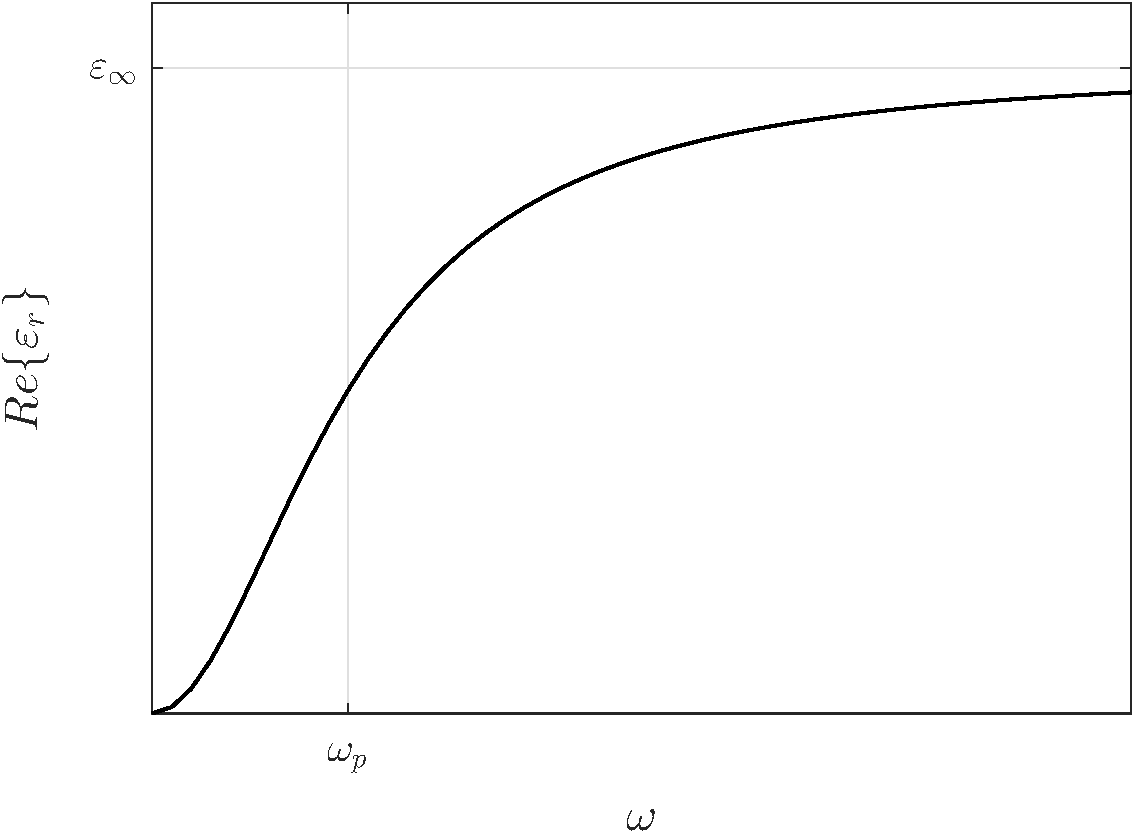
\includegraphics[width=\linewidth]{Figures/Chapters/PhysicalProblem/drudePermittivityReal}
  \captionof{figure}{First caption}
  \label{img1}
\end{minipage}
\hspace{.05\linewidth}
\begin{minipage}{.45\linewidth}
  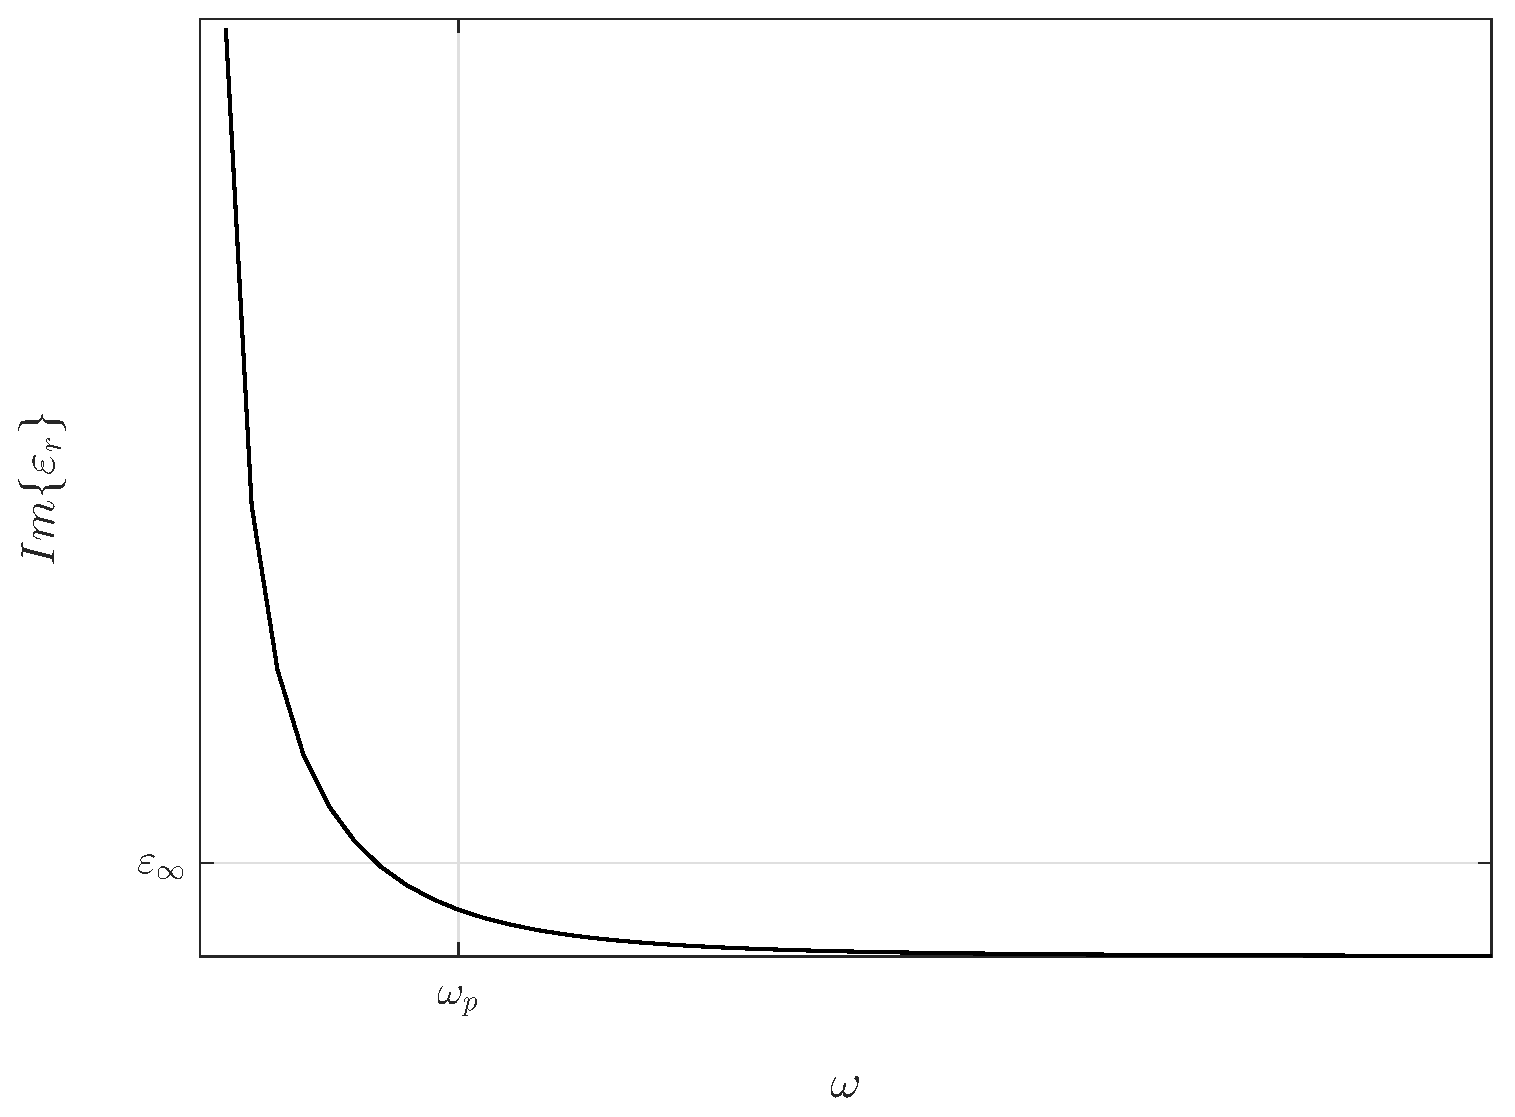
\includegraphics[width=\linewidth]{Figures/Chapters/PhysicalProblem/drudePermittivityImag}
  \captionof{figure}{Second caption}
  \label{img2}
\end{minipage}
\end{figure}
}


\usepackage{xparse}

\ExplSyntaxOn
% Usage:
% \twoimages{
%     {Chapters/figure/path}{figure caption},
%     {Chapters/figure/path}{another caption}
% }
\NewDocumentCommand{\twoimages}{ >{ \SplitList {,} } m }
 {
  \centering
  \ProcessList { #1 } { \__davs_process_argument:n }
 }
\cs_new_protected:Nn \__davs_process_argument:n
 {
  \__davs_image:nnn #1
 }
\cs_new_protected:Nn \__davs_image:nnn
 {
  \begin{subfigure}{0.45\textwidth}
    \centering
    \includegraphics[width=\textwidth]{Figures/#1}
    %\caption{#2}
    %\label{ris:#1}
  \end{subfigure} %
  \hfill
  \penalty0 % we provide a break point
 }
\ExplSyntaxOff
%%% Local Variables:
%%% mode: latex
%%% TeX-master: t
%%% End:


% enable previewing in emacs
\usepackage[displaymath,textmath,sections,graphics,floats]{preview}
\PreviewEnvironment{subequations}
%% ----------------------------------------------------------------
\begin{document}
\frontmatter	  % Begin Roman style (i, ii, iii, iv...) page numbering

% Set up the Title Page
\title  {Thesis Title}
\authors  {\texorpdfstring
            {\href{your web site or email address}{Author Name}}
            {Author Name}
            }
\addresses  {\groupname\\\deptname\\\univname}  % Do not change this here, instead these must be set in the "Thesis.cls" file, please look through it instead
\date       {\today}
\subject    {}
\keywords   {}

%\maketitle
%% ----------------------------------------------------------------

\setstretch{1.3}  % It is better to have smaller font and larger line spacing than the other way round

% Define the page headers using the FancyHdr package and set up for one-sided printing
\fancyhead{}  % Clears all page headers and footers
\rhead{\thepage}  % Sets the right side header to show the page number
\lhead{}  % Clears the left side page header

\pagestyle{fancy}  % Finally, use the "fancy" page style to implement the FancyHdr headers

%% ----------------------------------------------------------------
% % Declaration Page required for the Thesis, your institution may give you a different text to place here
\Declaration{

\addtocontents{toc}{\vspace{1em}}  % Add a gap in the Contents, for aesthetics

I, AUTHOR NAME, declare that this thesis titled, `THESIS TITLE' and the work presented in it are my own. I confirm that:

\begin{itemize} 
\item[\tiny{$\blacksquare$}] This work was done wholly or mainly while in candidature for a research degree at this University.
 
\item[\tiny{$\blacksquare$}] Where any part of this thesis has previously been submitted for a degree or any other qualification at this University or any other institution, this has been clearly stated.
 
\item[\tiny{$\blacksquare$}] Where I have consulted the published work of others, this is always clearly attributed.
 
\item[\tiny{$\blacksquare$}] Where I have quoted from the work of others, the source is always given. With the exception of such quotations, this thesis is entirely my own work.
 
\item[\tiny{$\blacksquare$}] I have acknowledged all main sources of help.
 
\item[\tiny{$\blacksquare$}] Where the thesis is based on work done by myself jointly with others, I have made clear exactly what was done by others and what I have contributed myself.
\\
\end{itemize}
 
 
Signed:\\
\rule[1em]{25em}{0.5pt}  % This prints a line for the signature
 
Date:\\
\rule[1em]{25em}{0.5pt}  % This prints a line to write the date
}
\clearpage  % Declaration ended, now start a new page
%% ----------------------------------------------------------------
% % The "Funny Quote Page"
\pagestyle{empty}  % No headers or footers for the following pages

\null\vfill
% Now comes the "Funny Quote", written in italics
\textit{``Write a funny quote here.''}

\begin{flushright}
If the quote is taken from someone, their name goes here
\end{flushright}

\vfill\vfill\vfill\vfill\vfill\vfill\null
\clearpage  % Funny Quote page ended, start a new page
%% ----------------------------------------------------------------
% % The Abstract Page
\addtotoc{Abstract}  % Add the "Abstract" page entry to the Contents
\abstract{
\addtocontents{toc}{\vspace{1em}}  % Add a gap in the Contents, for aesthetics

The Thesis Abstract is written here (and usually kept to just this page). The page is kept centered vertically so can expand into the blank space above the title too\ldots

}

\clearpage  % Abstract ended, start a new page
%% ----------------------------------------------------------------
%\setstretch{1.3}  % Reset the line-spacing to 1.3 for body text (if it has changed)

% The Acknowledgements page, for thanking everyone
\acknowledgements{
\addtocontents{toc}{\vspace{1em}}  % Add a gap in the Contents, for aesthetics

The acknowledgements and the people to thank go here, don't forget to include your project advisor\ldots

}
\clearpage  % End of the Acknowledgements

%% ----------------------------------------------------------------
 %%% ----------------------------------------------------------------
\lhead{\emph{List of Figures}}  % Set the left side page header to "List if Figures"
\listoffigures  % Write out the List of Figures

%% ----------------------------------------------------------------
\lhead{\emph{List of Tables}}  % Set the left side page header to "List of Tables"
\listoftables  % Write out the List of Tables

\pagestyle{fancy}  %The page style headers have been "empty" all this time, now use the "fancy" headers as defined before to bring them back


%% ----------------------------------------------------------------
\setstretch{1.5}  % Set the line spacing to 1.5, this makes the following tables easier to read
\clearpage  % Start a new page
\lhead{\emph{Abbreviations}}  % Set the left side page header to "Abbreviations"
\listofsymbols{ll}  % Include a list of Abbreviations (a table of two columns)
{
% \textbf{Acronym} & \textbf{W}hat (it) \textbf{S}tands \textbf{F}or \\
\textbf{LAH} & \textbf{L}ist \textbf{A}bbreviations \textbf{H}ere \\

}

%% ----------------------------------------------------------------
\clearpage  % Start a new page
\lhead{\emph{Physical Constants}}  % Set the left side page header to "Physical Constants"
\listofconstants{lrcl}  % Include a list of Physical Constants (a four column table)
{
% Constant Name & Symbol & = & Constant Value (with units) \\
Speed of Light & $c$ & $=$ & $2.997\ 924\ 58\times10^{8}\ \mbox{ms}^{-\mbox{s}}$ (exact)\\

}

%% ----------------------------------------------------------------
\clearpage  %Start a new page
\lhead{\emph{Symbols}}  % Set the left side page header to "Symbols"
\listofnomenclature{lll}  % Include a list of Symbols (a three column table)
{
% symbol & name & unit \\
$a$ & distance & m \\
$P$ & power & W (Js$^{-1}$) \\
& & \\ % Gap to separate the Roman symbols from the Greek
$\omega$ & angular frequency & rads$^{-1}$ \\
}

\lhead{\emph{Contents}}  % Set the left side page header to "Contents" 
\tableofcontents  % Write out the Table of Contents
%% ----------------------------------------------------------------
% % End of the pre-able, contents and lists of things
% Begin the Dedication page

\setstretch{1.3}  % Return the line spacing back to 1.3

\pagestyle{empty}  % Page style needs to be empty for this page
\dedicatory{For/Dedicated to/To my\ldots}

\addtocontents{toc}{\vspace{2em}}  % Add a gap in the Contents, for aesthetics
%% ----------------------------------------------------------------
\mainmatter	  % Begin normal, numeric (1,2,3...) page numbering
\pagestyle{fancy}  % Return the page headers back to the "fancy" style

% Include the chapters of the thesis, as separate files
% Just uncomment the lines as you write the chapters

%\chapter{Introduction} % Write in your own chapter title
\label{Chapter1}
\lhead{Chapter 1. \emph{Introduction}} % Write in your own chapter title to set the page header

Lots of motivation - this needs to be like a sales pitch to industry/goverment on why this research is important.
Refer to specific examples of cavities - this includes maybe acoustic cavities and EM ones and a lot of examples of lasers
Talk the need to make things SMALLER
AVOID WAFFLE - always refer to specific examples from literature - like a literature review.
What nanolasers (and cavities) have been simulated or built recently
Look for recent SPECIAL ISSUES or BOOKS on maybe resonance, cavities, nanolasers, EM cavities etc etc etc - look at the references.
ANYONE should be able to read this with NO expertise

\begin{itemize}
	\item what is the problem (resonant frequencies in a cavity)
	\item what is a cavity? where are they used? why are they relevant? - laser design
	\item industrial relevance - why is there need for research (nano/smaller)
  \item what are the quantities of interest in a cavity (res freq/QF/mode shapes)
\end{itemize}

\chapter{Physical Problem}
\label{PhysicalProblemChapter}
\lhead{Chapter 2. \emph{Physical Problem}} In this chapter, Maxwell's equations
of classical electrodynamics are introduced, both in integral and differential
forms. The wavelengths of interest are sufficiently large, with respect to
atomic scale variations in the medium, that a macroscopic approach is justified
and quantum mechanical effects are neglected. Constitutive equations will be
introduced for linear, isotropic material both with and without dispersive
effects. Following this, we introduce the Drude model and use it to incorporate
frequency-dependent interactions into Maxwell's equations in a formulation
suitable for efficient numerical calculation. The conditions which must be
satisfied at material interfaces will be derived and alternative forms of
Maxwell's equations discussed.

\section{Maxwell's equations}
The classical theory of electrodynamics decribes the behaviour evolution of
electromagnetic radiation using Maxwell's unification of the equations of
electrodynamics\cite{Balanis:ui,Jackson:490457}. The resulting coupled
equations, which govern the time evolution of electromagnetic waves, are known
collectively as Maxwell's equations, and written in standard units as
\begin{subequations}
  \begin{align}
    \int_{\partial S} \Etilde(\xbftilde,\ttilde) \cdot \vectdl  &= - \frac{d}{dt} \int_{S} \Btilde(\xbftilde,\ttilde) \cdot \vectdS, \label{eq:maxwell-faraday-integral} \\
    \int_{\partial S} \Btilde(\xbftilde,\ttilde) \cdot \vectdl &= \mu_0 \eps_0 \frac{d}{dt} \int_{S} \Etilde(\xbftilde,\ttilde) \cdot \vectdS +  \mu_0 \int_{S} \Jtilde(\xbftilde,\ttilde) \cdot \vectdS, \label{eq:maxwell-ampere-integral} \\
    \int_{\partial \Vol} \Dtilde(\xbftilde,\ttilde)\cdot\vectdS &= \int_\Vol \rho \,\dV, \label{eq:maxwell-gauss-integral} \\
    \int_{\partial \Vol} \Btilde(\xbftilde,\ttilde)\cdot\vectdS &= 0, \label{eq:maxwell-gauss-magnetism-integral}
  \end{align}
\end{subequations}
where $\xbftilde$ is the position vector, $\ttilde$ is time in seconds, $\eps_0$
is the permittivity of free space in farads per meter, $\mu_0$ is the
permeability of free space in henries per meter and the vectors $\Etilde$,
$\Htilde$, $\Dtilde$ and $\Btilde$ are used to denote respectively the electric
field intensity in volts per meter, magnetic field intensity in amps per meter,
electric displacement in coulombs per meter squared, and magnetic induction in
weber per meter squared. $\rho$ denotes volume charge density in coloumb per
meter cubed and $\Jtilde$ denotes electric current density in ampere per meter
squared.
% VIVA: these are BOTH due to EXTERNAL charge only, this means not due to
% induced effects (e.g polarisation) QUOTE: both denote sources due to free
% charges in the system
$\Vol$ denotes any closed volume while the infinitesimal integration elements
$\vectdl$, $\vectdS$ and $\dV$ are respectively a line element, vector surface
element and volume element.
% "In regions where the material parameters are differentiable"... -> but hang
% on! The material parameters are not involved here. What restrictions are the
% for using Stokes' Theorem?
By applying Stokes' Theorem to~\eqref{eq:maxwell-faraday-integral}
and~\eqref{eq:maxwell-ampere-integral} and Gauss' law
to~\eqref{eq:maxwell-gauss-integral}
and~\eqref{eq:maxwell-gauss-magnetism-integral}, the equations in differential
form are obtained as
\begin{subequations}
  \label{eq:maxwells-equations-diff}
  \begin{align}
    \nablatilde \times \Etilde(\xbftilde,\ttilde) + \dpartttilde{\Btilde(\xbftilde, \ttilde)}&= \mathbf{0}, \label{eq:maxwell-faraday} \\
    \nablatilde \times \Htilde(\xbftilde,\ttilde) - \dpartttilde{\Dtilde(\xbftilde, \ttilde)}&= \Jtilde(\xbftilde,\ttilde), \label{eq:maxwell-ampere} \\
    \nablatilde \cdot \Dtilde (\xbftilde,\ttilde) &= \rho(\xbftilde,\ttilde), \label{eq:maxwell-gauss-1}, \\
    \nablatilde \cdot \Btilde (\xbftilde,\ttilde) &= 0, \label{eq:maxwell-gauss-2} .
  \end{align}
\end{subequations}
Where the operator $\nablatilde \times$ and $\nablatilde \cdot$ denote
respectively taking the curl and taking the divergence, both with respect to the
position vector $\xbftilde$. The four equations
in~\eqref{eq:maxwells-equations-diff} are known respectively as Ampere's law
with Maxwell's correction, Faraday's law, Gauss' law and Gauss' law for
magnetism. These are classified as Maxwell's curl
equations,in~\eqref{eq:maxwell-ampere} and~\eqref{eq:maxwell-faraday}, which
determine the evolution of the vector fields in time, and Maxwell's divergence
conditions,in~\eqref{eq:maxwell-gauss-1} and~\eqref{eq:maxwell-gauss-2}, which
are constraints on $\Dtilde$ and $\Btilde$, which should be satisfied at each
point in time.

\subsection{Conservation of charge}
Conservation of charge can be derived directly from Maxwell's equations. The
vector identity
\begin{equation}
  \label{eq:vector-identity-1}
  \nablatilde \cdot ( \nablatilde \times \mathbf{A} (\xbftilde) ) = 0,
\end{equation}
which holds for any vector field $\mathbf{A}$, is substituted into the
expression obtained by taking the divergence of both sides of Ampere's
law,~\eqref{eq:maxwell-ampere}, giving:
$$
- \dpartttilde{( \nablatilde \cdot \Dtilde(\xbftilde,\ttilde) ) } = \nablatilde
\cdot \Jtilde(\xbftilde,\ttilde) .
$$
By substituting Gauss' law,~\eqref{eq:maxwell-gauss-1}, into this equation we
obtain the following conservation equation for charge
\begin{equation}
  \label{eq:maxwell-charge-conservation-2}
  \nablatilde \cdot \Jtilde(\xbftilde,\ttilde) + \dpartttilde{\rho (\xbftilde,\ttilde) } = 0 .
\end{equation}
Taking the divergence of Amperes law,~\eqref{eq:maxwell-ampere}, and removing
the curl term by recalling the identity~\eqref{eq:vector-identity-1}, results in
$$
\nablatilde \cdot \dpartttilde{ \Dtilde(\xbftilde, \ttilde)} = - \nablatilde
\cdot \Jtilde(\xbftilde,\ttilde),
$$
which can be rewritten using the conservation of charge
equation,~\eqref{eq:maxwell-charge-conservation-2}, as
$$
\nablatilde \cdot \dpartttilde{\Dtilde(\xbftilde, \ttilde)} = - \dpartttilde{
  \rho (\xbftilde,\ttilde)}.
$$
Following a similar procedure using~\eqref{eq:maxwell-faraday} results in
$$
\nablatilde \cdot \dpartttilde{ \Btilde(\xbftilde, \ttilde)} = 0
$$

Thus provided the initial conditions satisfy equation Maxwell's divergence
conditions,~\eqref{eq:maxwell-gauss-1} and~\eqref{eq:maxwell-gauss-2}, and the
conservation of charge equation,~\eqref{eq:maxwell-charge-conservation-2}, is
satisfied at all times then if the system is evolved in time using Maxwell's
curl equations alone the divergence conditions will be implicitly satisfied at
all times.

\section{Constitutive equations}
\label{Ch:PhysicalProblem:ConstitutiveEquations}
Maxwell's equations in differential form,~\eqref{eq:maxwells-equations-diff},
are an underdetermined system of equations, with 4 equations and 6 unknowns. The
system of equations is closed by macroscopic constitutive laws, written as
% VIVA: this is not true for materials which exhibit ferromagnetic or
% ferroelectric behaviour - but this is a quantum effect, so outside of our
% classical scope. what are the constitutive laws in this case?
\begin{subequations}
  \begin{align}
    \Dtilde(\xbftilde,\ttilde) &= \eps_0 \Etilde(\xbftilde,\ttilde) + \Ptilde\left[ \Etilde, \Htilde, \xbftilde, \ttilde \right]  \label{eq:constitutive-general-E}\\
    \Btilde(\xbftilde,\ttilde) &= \mu_0 \Htilde(\xbftilde,\ttilde) + \Mtilde\left[ \Etilde, \Htilde, \xbftilde, \ttilde \right] \label{eq:constitutive-general-H}
  \end{align}
\end{subequations}
where $\Ptilde$, the polarisation density, and $\Mtilde$, the magnetisation
density, quantify the change in $\D$ and $\B$ resulting from the interaction
between the applied electromagnetic fields and the medium.
% However, for a given material the dependence may be non-local in space,
% non-local in time, non-linear, and/or anisotropic.
The polarisation and magnetisation densities for linear, isotropic and media
with frequency-independent material properties are described as
\begin{subequations}
  \begin{align}
    \Ptilde &= \ElecSuccept(\xbftilde) \Etilde(\xbftilde,\ttilde), \label{eq:elec-susceptibilities-definition-E} \\
    \Mtilde &= \MagSuccept(\xbftilde) \Htilde(\xbftilde,\ttilde) . \label{eq:elec-susceptibilities-definition-H} 
  \end{align}
\end{subequations}
where $\ElecSuccept$, the electric suceptibility, and $\MagSuccept$, the
electric susceptibility, are a measure of polarisation or magnetisation of the
medium in response and applied fields.
Using~\eqref{eq:elec-susceptibilities-definition-E}
and~\eqref{eq:elec-susceptibilities-definition-H}, the constitutive equations,
shown in~\eqref{eq:constitutive-general-E}
and~\eqref{eq:constitutive-general-H}, can be rewritten in the simple form
\begin{subequations}
  \label{eq:constitutive-linear}
  \begin{align}
    \Dtilde(\xbftilde,\ttilde) = \eps_0 \eps_r(\xbftilde) \Etilde(\xbftilde,\ttilde), \label{eq:constitutive-linear-D} \\
    \Btilde(\xbftilde,\ttilde) = \mu_0 \mu_r(\xbftilde) \Htilde(\xbftilde,\ttilde),\label{eq:constitutive-linear-B}
  \end{align}
\end{subequations}
where the material response is completely characterised by two dimensionless
scalars $ \eps_r, \mu \in \Real$, known respectively as the permittivity and the
relative permeability, given by $\eps_r \equiv 1 + \ElecSuccept $ and $\mu_r
\equiv 1 + \MagSuccept $.
% TODO - cite{Maier:5SXqSjV8} -> copied

\subsection{Dispersive Drude Media}
Most media exhibits frequency dependence of both $\eps_r$ and $\mu_r$, a
phenomena known as dispersion, which arises due to the finite time the medium
needs to repond to changes in applied electromagnetic fields. Whilst dispersive
effects are generally neglected in simulations of dielectrics, many metals of
interest in photonics, such as gold, silver and aluminum, have strongly
frequency dependent relative permittivities in the visible and infra-red regions
of the electromagnetic spectrum\cite{Ordal:1983bg}. This is a consequence of the
finite time required for charged particles in the medium to reach a equilibrium
positions in the presence of a changing applied electromagnetic field. In these
cases, the electric susceptibility can no longer be written as a function of
$\xbftilde$ only, but is expressed as convolution integrals in
time\cite{Jackson:490457}.
% VIVA: article - A comparison of numerical techniques for modeling well
For metals where the effects of interband electron transitions are negligible, a
mechanical model based on the Drude model of solids is
sufficient\cite{taflove2013advances}. For more complex material interactions
however, a more sophisticated model such as the Drude-Lorentz
model\cite{Fox:2001wm,Taflove:1989ds} or approaches based on the
$Z$-transform\cite{sullivan1996z} may be used. We restrict the follow discussion
to media and frequency ranges where magnetisation effects are
frequency-independent, and thus~\eqref{eq:constitutive-linear-B} remains valid,
and where polarisation can be approximated by a single-pole Drude model.

%% *** ## "Polarisation density also describes how a material responds to an
%% applied electric field as well as the way the material changes the electric
%% field, and can be used to calculate the forces that result from those
%% interactions."
% ...based on the kinetic theory of gases,
%
% *** "The induced polarisation due to frequency-dependent electron movement
% leads to a frequency-dependent polarisation (dispersion)" - ref Maier
%
% Electron-ion collisions are random events, with a probability $dt / \tau$ (tau
% is the inv of gamma) - following which the electron velocities are independent
% of velocities prior to collision.
A Drude medium is composed of a lattice of fixed-position, positively charged
ions bound by a delocalised sea of valence band free
electrons\cite{Ashcroft:2005wp,Bandyopadhyay:1503732}. The free electrons,
following the kinetic theory of ideal gases, are non-interacting, independent
particles, described by Newtonian mechanics. In the presence of the electric
field, $\Etilde$, the ions remain fixed and only the free electrons are
displaced from their zero-field equilibrium positions. In the Drude model
polarisation arises from two independent sources: a frequency-independent
background polarisation, $\PtildeInf$, due to the fixed-position charged ions,
and a frequency dependent free electron polarisation, $\PtildeElec$, due to the
delocalisation of free electrons in the presence of an electric field. Thus we
begin by writing~\eqref{eq:constitutive-general-E} in the frequency domain as
\begin{align}
  \hat{\Dtilde}(\xbftilde,\omega) &= \eps_0 \hat{\Etilde}(\xbftilde, \omega) + \PtildeInfFreq + \PtildeElecFreq(\xbftilde,\omega) ,
                                    \label{eq:constitutive_equations_drude_model}
\end{align}
where $\omega$ is the frequency variable and a circumflex denotes the frequency
domain representation of a time domain quantity, such that
$$
\hat{\Box}(\xbftilde,\omega) = \int_{-\infty}^{+\infty} \Box(\xbftilde,\ttilde)
e^{-i \omega t} dt
$$
where the real-valued function $\Box$ of the temporal variable, $\ttilde \in
\Real$, has been written as the complex valued function $\hat{\Box}$ of angular
frequency, $\omega \in \Real$, which is related to frequency, $f$, by $\omega =
2 \pi f$. Note in particular that $- i \omega \hat{\Box}(\xbftilde,\omega) =
\dpartt{ \Box(\xbftilde,\ttilde) }$. Since $\PtildeInfFreq$ is
frequency-independent, following the procedure
from~\autoref{Ch:PhysicalProblem:ConstitutiveEquations}, we
rewrite~\eqref{eq:constitutive_equations_drude_model} as
\begin{equation}
  \hat{\Dtilde}(\xbftilde,\omega) = \eps_0 \eps_{\infty} \hat{\Etilde}(\xbftilde, \omega) + \hat{\Ptilde}_e(\xbftilde,\omega) ,
\end{equation}
where $\eps_{\infty} \equiv 1 + \ElecSucceptInf $ is the permittivity in the
infinite frequency limit, and $\ElecSucceptInf$ is defined by $\PtildeInfFreq
\equiv \eps_0 \ElecSucceptInf \hat{\Etilde} $.
Transforming~\eqref{eq:constitutive_equations_drude_model} directly to the time
domain would lead to a convolution integral, which presents challenges for
numerical simulation\cite{kelley1996piecewise}. We instead follow the so called
Auxiliary Differential Equation (ADE)
approach\cite{Taflove:1989ds,Niegemann:2009uv,Ji:2007dl,okoniewski1997simple,kashiwa1990treatment}.
First we define the current due to free electron polarisation, $\Jtildep$, as
\begin{align}
  \Jtildep(\xbftilde,\ttilde) =  \dpartt{\Ptilde}_e(\xbftilde,\ttilde). \label{eq:polarisation-current-definition}
\end{align}
By multiplying~\eqref{eq:constitutive_equations_drude_model} by $ -i \omega$ and
then transforming it to the time domain, we obtain a constitutive relation in
the form of an ordinary differential equation
\begin{equation}
  \label{eq:constitutive_equations_drude_model_derivative_TD}
  \dodettilde{ \Dtilde (\xbftilde,\ttilde) }= \eps_0 \eps_{\infty} \dodettilde{ \Etilde (\xbftilde, \ttilde) } + \Jtildep(\xbftilde,\ttilde) .
\end{equation}
% TODO - check that the - is correct in this definition, and that J is defined
% in the opposite direction to P
By substitution into Ampere's law,~\eqref{eq:maxwell-ampere}, we obtain the
expression
\begin{align}
  \nablatilde \times \Htilde(\xbftilde,\ttilde) - \dpartttilde{\Dtilde_{\infty}(\xbftilde, \ttilde)} &= \Jtilde(\xbftilde,\ttilde) + \Jtildep(\xbftilde,\ttilde) , \label{eq:drude-ampere}
\end{align}
where, to maintain consistency with dispersion-free form of Maxwell's
equations~\eqref{eq:maxwells-equations-diff} we have defined $\Dtilde_{\infty}
\equiv \eps_0 \eps_{\infty} \Etilde$, as the electric displacement in the
infinite frequency limit.

Motivated by the Drude model, and recalling that that the motion of each
electron is independent, we derive an expression for $\Jtildep$ from the
Newtonion equations of motion of a free electron in the presence of a
time-varying applied field, $\EappliedDrude(\ttilde)$. We note that the
polarisation field due to electron movement is related to the displacemment,
$\xdispelecvect$, of an electron from its zero-field equilibrium position by $
\PtildeElec(\ttilde) = - n q \xdispelecvect(\ttilde) $, where $n$ is the
electron density in the medium. Thus, the Newtonian equations of motion electon
describing the displacement of an electon can be written directly in terms of
polarisation as
\begin{equation}
  \label{eq:equations-of-motion-electron}
  \frac{d^2 \PtildeElec(\ttilde) }{dt^2} + \gamma \frac{d \PtildeElec(\ttilde) }{dt} = - \eps_0 \plasfreq^2 \EappliedDrude(\ttilde),
\end{equation}
where $\gamma$ is a damping coefficient or collision frequency, $m_e$ is the
mass of an electron, $q$ is the charge of an electron, and $\plasfreq \equiv
\sqrt{\frac{n q^2}{m_e \eps_0}}$ is known as the plasma frequency.
% TODO - is it ok to write directly in terms of polarisation (or is this
% ignoring something?) Do I genuinely neglect electron interactions? Another
% approaches I've seen is using a single freuqnecy (monochromatic field
% \Etilde(\xbftilde,\ttilde) = \hat{\mathbf{E_0}} e^{- i \omega \ttilde} TODO -
% what is the plasma frequency physically
From the definition of $\Jtildep$ given
in~\eqref{eq:polarisation-current-definition}, we
~\eqref{eq:polarisation-from-P} can be written as
\begin{equation}
  \dpartttilde{\Jtildep(\xbftilde,\ttilde)} + \gamma \Jtildep(\xbftilde) = \eps_0 \plasfreq^2 \Etilde(\xbftilde,\ttilde).
  \label{eq:pol-current-ADE}
\end{equation}

Maxwell's curl equations and constitutive equations in a Drude dispersive
medium, are given by
\begin{subequations}
  \label{eq:dispersive-maxwell-system}
  \begin{align}
    \nablatilde \times \Etilde(\xbftilde,\ttilde) + \dpartttilde{ \Btilde(\xbftilde, \ttilde)}&= 0, \\
    \nablatilde \times \Htilde(\xbftilde,\ttilde) - \dpartttilde{ \Dtilde_{\infty}(\xbftilde, \ttilde) }&= \Jtilde(\xbftilde,\ttilde) - \Jtildep(\xbftilde,\ttilde), \\
    \Dtilde_{\infty}(\xbftilde,\ttilde) &= \eps_0 \eps_{\infty}(\xbftilde) \Etilde(\xbftilde,\ttilde), \\
    \Btilde(\xbftilde,\ttilde) &= \mu_0 \mu_r(\xbftilde) \Htilde(\xbftilde,\ttilde), \\
    \frac{d \Jtildep(\xbftilde)}{dt} + \gamma \Jtildep(\xbftilde) &= - \eps_0 \plasfreq^2 \Etilde(\xbftilde, \ttilde) . \label{eq:maxwell-dispersive-ADE}
  \end{align}
\end{subequations}
We note that these equations reduce to the non-dispersive case, given
in~\eqref{eq:maxwell-ampere},~\eqref{eq:maxwell-faraday}
and~\eqref{constitutive-linear} in the infinite frequency limit.

Some insight into the behaviour of Drude metals can be obtained by looking at
the relative permittivity obtained in the frequency domain.
First,~\eqref{eq:polarisation-from-P-FD} can be rearranged to obtain the
polarisation due to free electrons in the frequency domain,
\begin{equation}
  \hat{\Ptilde}_e = - \frac{\eps_0 \plasfreq^2}{\omega^2 - i \omega \gamma } \hat{\Etilde}(\omega) .
  \label{eq:polarisation-field-freq-domain}
\end{equation}
Using this expression,~\eqref{eq:constitutive_equations_drude_model} may be
rewritten explicitly in the frequency domain as
\begin{equation}
  \begin{split}
    \hat{\Dtilde}(\xbftilde,\omega) &= \eps_0 \left( \eps_{\infty} - \frac{\plasfreq^2 }{\omega^2 - i \omega \gamma } \right) \hat{\Etilde}(\omega) \\
    &= \eps_0 \hat{\eps}_r (\omega) \hat{\Etilde}(\omega) ,
  \end{split}
\end{equation}
where $\hat{\eps}_r(\omega)$ is the effective permittivity of the metal. Figure
\ref{fig:read-and-imag-effective-permittivity} shows the real and imaginary
parts of $\hat{\eps}_r$, given by
\begin{subequations}
  \begin{align}
    Re\{ \hat{\eps}_r \} &= \eps_{\infty} - \frac{\plasfreq^2}{\omega^2 + \gamma^2}, \\
    Im\{ \hat{\eps}_r \} &= \frac{\gamma \plasfreq}{\omega ( \omega^2 + \gamma^2) } ,
  \end{align}
\end{subequations}
plotted against normalised angular frequency $\omega / \plasfreq$. We observe
that at higher frequencies, due to reduced electron motion, the non-dispersive
dielectric behaviour is recovered as $Re\{\hat{\eps}_r\} \to \eps_{\infty}$ and
$Im\{\hat{\eps}_r\} \to 0$. For frequencies below $\plasfreq$ however, the real
and imaginary parts of the permittivity diverge significantly from the
dispersive values. The positive values of the imaginary part result in an
attenuation of the electric field amplitude in this region.

\begin{figure}[htbp!]
  \begin{center}
    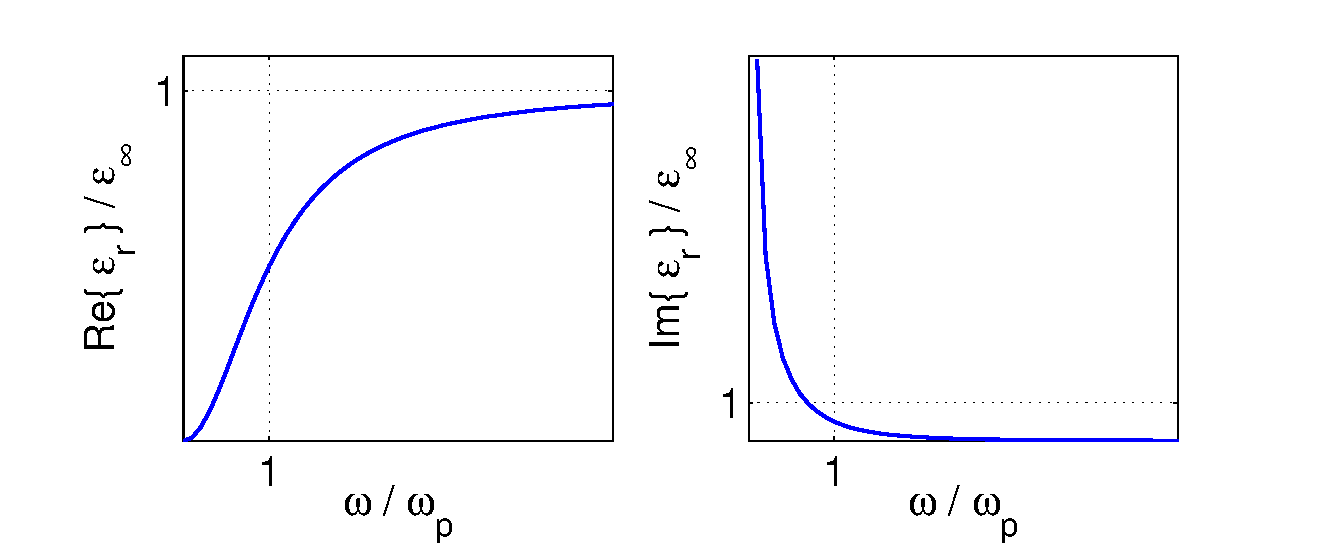
\includegraphics[scale=0.7]{Figures/Chapters/PhysicalProblem/drudePermittivity}
  \end{center}
  \caption{The real (left) and imaginary (right) parts of the dispersive
    frequency domain relative permittivity, $\hat{\eps}_r$, as obtained from
    Drude model.}
  \label{fig:read-and-imag-effective-permittivity}
\end{figure}

\section{Dimensionless form}
% "\eps_0 and \mu_0 introduces an arbitraryness of dimension which we exploit
% for the dimensionless form"
Maxwell's equations are not invariant under change of units, with the constants
$\eps_0$, $\mu_0$ and changing value and position. Unit systems in common use
include the SI units used above, Gaussian units, Lorentz-Heaviside units and
Planck units. In particular, for numerical simulations, dimensionless unit
systems are useful to avoid rounding errors in floating point arithmetic. Maxwell's equations can be obtained in dimensionless form by scaling length and
time by an arbitrary characteristic length, $L$. The following changes of
variable are introduced:
\begin{align}
  \label{eq:dimensionless-scaling-1}
  \xbf &= \frac{\xbftilde}{\charLen}, &  \
                                        t &= \frac{\czero \ttilde}{\charLen}, &  \
                                                                                \plasfreq &= \frac{\plasfreqtilde \charLen}{\czero}, & \
                                                                                                                                       \gamma &= \frac{\gammatilde \charLen}{\czero},
\end{align}
where $\czero = ( \eps_0 \mu_0 )^{-\frac{1}{2}}$ is the speed of light in vacuum
in SI units, and the quantities $\xbf$ and $\t$ have been chosen such that the
dimensionless speed of light in vacuum is unity. Additionally, electromagnetic
field strengths and currents may be scaled by a characteristic field strength,
$\E_0$, by introducing the following dimensionless variables:
\begin{align}
  \label{eq:dimensionless-scaling-2}
  \E &= \Etilde, &  \
                   \H &= \intImpFS \Htilde, &  \
                                              \J &= \charLen \intImpFS \Jtilde, & \
                                                                                  \J_p &= \charLen \intImpFS \Jtilde_p,
\end{align}
% note - could also scale all of these values with E_0
where $\eta_0 = \sqrt{\mu_0 / \eps_0}$ is the intrinsic impedence of free space. Derivatives with respect to $\ttilde$ and $\xbftilde$ are transformed as
\begin{align}
  \label{eq:dimensionless-scaling-3}
  \dpartttilde{\Box} &= \frac{\czero}{\charLen}\dpartt{\Box}, & \
                                                                \dpartxtilde{\Box} &= \frac{1}{\charLen}\dpartx{\Box}
\end{align}
By substitution of~\eqref{eq:dimensionless-scaling-1} and~\eqref{eq:dimensionless-scaling-2} into Maxwell's curl
equations,~\eqref{eq:maxwell-ampere} and~\eqref{eq:maxwell-faraday}, we obtain
the curl equations modified for dispersive materials in dimensionless form:
\begin{subequations}
  \label{eq:dimensionless-maxwell}
  \begin{align}
    \nabla \times \E(\xbf,\t) + \dpartt{\B(\xbf, \t) } &= 0, \\
    \nabla \times \H(\xbf,\t) - \dpartt{ \D_{\infty}(\xbf, \t) } &=  \J_p(\xbf,\t), \\
    \D_{\infty}(\xbf,\t) &= \eps_{\infty}(\xbf) \E(\xbf,\t), \\
    \B(\xbf,\t) &= \mu_r(\xbf) \H(\xbf,\t), \\
    \frac{d \J_p(\xbf,\t)}{d\t} + \gamma \J_p(\xbf,\t) &= \omega_p^2 \E(\xbf,\t),
  \end{align}
\end{subequations}
where $\DInf$ and $\B$ are the appropriately scaled values of $\DtildeInf$ and
$\Btilde$. Note that the non-dispersive form may be recovered in the infinite
frequency limit, where $\J_p = 0$, $\eps_{\infty} = \eps_r$ and $\DInf = \D$
equations,~\eqref{eq:maxwells-equations-diff}, to obtain the equivalent
non-dispersive dimensionless form.

\section{Conservation form}

% *** EVERYTHING WRITTEN AS FREE SPACE - \mu = 1 probably ok for my examples but
% \eps != 1 ***
The dispersive form of Maxwell's equations in dimensionless
form,~\eqref{eq:dimensionless-maxwell}, can be conveniently rewritten as a
linear, hyperbolic conservation law\cite{Godlewski:2013tj,LeVeque:2002vc}
% TODO - Ruben: need to show that system is hyperbolic (and linear?)
\begin{equation}
  \dpartt{ \, \USoltn} + \sum_{k=1}^{nsd} \frac { \partial \, \Flux_k(\USoltn) }{ \partial x_k } = \maxwellSource\,(\USoltn) \: ,
  \label{eq:maxwell-curl-equations-conservation-form}
\end{equation}
where $nsd$ denotes the number of spatial dimensions. The vector of unknowns,
$\USoltn$, the flux vectors, $\Flux_k$, and the source $\maxwellSource$ are
given by
\begin{equation*}
  \begin{array}{c}
    \USoltn =
    \begin{pmatrix}
      \eps_{\infty} E_1, \: \eps_{\infty} E_2 , \: \eps_{\infty} E_3 , \: \mu
      H_1 , \: \mu H_2 , \: \mu H_3 , \: \Jpol_1 , \: \Jpol_2 , \: \Jpol_3
    \end{pmatrix}^T,
    \\
    \Flux_1 =
    \begin{pmatrix}
      0 ,\: H_3 ,\: -H_2 ,\: 0 ,\: -E_3 ,\: E_2 ,\: 0 ,\: 0 ,\: 0
    \end{pmatrix}^T , \\

    \Flux_2 =
    \begin{pmatrix}
      - H_3 ,\: 0 ,\: H_1 ,\: E_3 ,\: 0 ,\: -E_1 ,\: 0 ,\: 0 ,\: 0
    \end{pmatrix}^T , \\

    \Flux_3 =
    \begin{pmatrix}
      H_2 ,\: -H_1 ,\: 0 ,\: -E_2 ,\: E_1 ,\: 0 ,\: 0 ,\: 0 ,\: 0
    \end{pmatrix}^T , \\

    \maxwellSource =
    \begin{pmatrix}
      J_1 + \Jpol_1 ,\: J_2 + \Jpol_2 ,\: J_3 + \Jpol_3 ,\: 0 ,\: 0 ,\: 0 ,\: \omega^2
      \: E_1 - \gamma \Jpol_1 ,\: \omega^2 \: E_2 - \gamma \Jpol_2 ,\: \omega^2 \:
      E_3 - \gamma \Jpol_3
    \end{pmatrix}^T,

  \end{array}
\end{equation*}
where $E_k$, $H_k$ and $\Jpol_k$ are the $k$th spatial components of the
dimensionless intensity vectors of electric field, magnetic field and the
polarisation current, respectively. The material parameters $\eps$, $\mu$,
$\omega$ and $\gamma$ are the electric permittivity, magnetic permeability,
plasma frequency and electron damping coefficient, respectively. The same form
may be used for non-dispersive cases, by setting $\Jpol_k = 0 \; \forall \; k$ and
setting $\eps_{\infty} = \eps_{r}$. The equations can be written in quasilinear
form
\begin{equation}
  \label{eq:quasilinear-form}
  \dpartt{\USoltn}  + \sum_{k=1}^{\nsd}\AQuasiLinear_k\dpart{\xbf_k}{\USoltn} = \AQuasiLinear_s \USoltn
\end{equation}
where

\begin{align}
  \AQuasiLinear_k = 
  \begin{pmatrix}
    \zerov & \RQuasiL_{k} & \zerov \\
    -\RQuasiL_{k} & \zerov & \zerov \\
    \zerov & \zerov & \zerov \\
  \end{pmatrix}
  \: \:
  \textrm{and}\;\;\;
  \AQuasiLinear_s = 
  \begin{pmatrix}
    \zerov  & \zerov & -\IdentityVect\\
    \zerov & \zerov & \zerov \\
    -\plasfreq \IdentityVect & \zerov & - \gamma \IdentityVect \\
  \end{pmatrix}
\end{align}
with
\begin{align}
  \RQuasiL_1 = 
  \begin{pmatrix}
    0 & 0 & 0 \\
    0 & 0 & 1 \\
    0 & -1 & 0 \\
  \end{pmatrix} , \: \: & \RQuasiL_2 =
                          \begin{pmatrix}
                            0 & 0 & -1 \\
                            0 & 0 & 0 \\
                            1 & 0 & 0 \\
                          \end{pmatrix}
      &
        \textrm{and   } \:\:\:
          &
            \RQuasiL_3 = 
            \begin{pmatrix}
              0 & 1 & 0 \\
              -1 & 0 & 0 \\
              0 & 0 & 0 \\
            \end{pmatrix}
      &
\end{align}

A system written in quasilinear form,~\eqref{eq:quasilinear-form}, is said to be hyperbolic if all the eigenvalue of the linear combination $ \AQuasiLinearComb \equiv \sum_{k} a_{k} \AQuasiLinear_k $ are real for any $a_{k} \in \Real$ and the matrix $\AQuasiLinearComb$ is diagonalisable. In $3$-dimensions the matrix $\AQuasiLinearComb$ is given by
$$
  \AQuasiLinearComb =
  \begin{pmatrix}
 & \zerov , & \RTot, & \zerov \\
 & -\RTot & \zerov & \zerov \\
 & \zerov & \zerov & \zerov 
 & \end{pmatrix}
$$
with
$$
  \RTot =
  \begin{pmatrix}
 & 0 & a_3 & -a_2 \\
 & -a_3 & 0 & a_1 \\
& a_2 & -a_1 & 0 
 & \end{pmatrix} .
$$
By writing the characteristic equation,

$$
  \begin{vmatrix}
 & -\lambda \IdentityVect, & \RTot, & \zerov \\
 & -\RTot & -\lambda \IdentityVect & \zerov \\
 & \zerov & \zerov & -\lambda \IdentityVect
 & \end{vmatrix}
= 0
$$
it can be easily shown that the eigenvalues, $\lambda_{i}$, take the values $0$ and $\pm \sqrt{a_1^2 + a_2^2 + a_3^2}$.

% or equivalently as
% $$
% \lambda^5 (a_{1}^2 + a_{2}^2 + a_{3}^2 - \lambda^2)^2 = 0
% 
% $$
% TODO - quasilinear form for TE and TM

\section{Reduction to 2 dimensions}
\subsection{TE and TM modes}
For a physical system where the electric field is translationally invariant in
the $z$-direction, the derivatives with respect to $z$ are zero. Maxwell's
equations are decoupled into two sets of coupled equations with three unknowns
each. The resulting modes in dimensionless form, accounting for dispersion with
the Drude model, are known as the $TE_z$ and $TM_z$ modes.

The $TE_z$ mode is given by

\begin{equation*}
  \begin{array}{ccccc}
    \USoltn_1 = \begin{pmatrix} \eps E_1 \\ \eps E_2 \\ \mu H_3 \\ \JpolScalar_1 \\  \JpolScalar_2 \end{pmatrix} ,
 &
   \Flux_1 = \begin{pmatrix} 0 \\ H_3 \\ E_2 \\ 0 \\  0 \end{pmatrix} ,
 &
   \Flux_2 = \begin{pmatrix} - H_3 \\ 0 \\ -E_1 \\ 0 \\ 0 \end{pmatrix} ,
 &
   \maxwellSource = \begin{pmatrix} J_1 + \JpolScalar_1 \\ J_2+ \JpolScalar_2 \\ 0 \\ \omega^2 \, E_1 - \gamma \JpolScalar_1 \\  \omega^2 \, E_2 - \gamma \JpolScalar_2 \end{pmatrix} ,
  \end{array}
  \:
\end{equation*}

or in quasilinear form,~\eqref{eq:quasilinear-form}, as 
\begin{align*}
  \AQuasiLinear_1 = 
  \begin{pmatrix}
    0 & 0 & 0 & 0 & 0 \\
    0 & 0 & 1 & 0 & 0 \\
    0 & 1 & 0 & 0 & 0 \\
    0 & 0 & 0 & 0 & 0 \\
    0 & 0 & 0 & 0 & 0 \\
  \end{pmatrix}
  \: \:
  \AQuasiLinear_2 = 
  \begin{pmatrix}
    0 & 0 &-1 & 0 & 0 \\
    0 & 0 & 0 & 0 & 0 \\
   -1 & 0 & 0 & 0 & 0 \\
    0 & 0 & 0 & 0 & 0 \\
    0 & 0 & 0 & 0 & 0 \\
  \end{pmatrix}
  \textrm{and}\;\;\;
  \AQuasiLinear_s = 
  \begin{pmatrix}
    0 & 0 & 0 & \Jnormalised{1} & 0 \\
    0 & 0 & 0 & 0 & \Jnormalised{2} \\
    0 & 0 & 0 & 0 & 0 \\
    \plasfreq^2 & 0 & 0 & -\gamma & 0 \\
    0 & \plasfreq^2 & 0 & 0 & -\gamma \\
  \end{pmatrix}
\end{align*}
where $\Jnormalised{k} = 1 + \frac{J_{k}}{\JpolScalar_{k}}$. The $TE_z$ mode is given by

\begin{equation*}
  \begin{array}{ccccc}
    \USoltn = \begin{pmatrix} \mu H_1 \\ \mu H_2 \\ \eps E_3 \\ \Jpol_3 \end{pmatrix} ,
 &
   \Flux_1 = \begin{pmatrix} 0 \\ -E_3 \\ -H_2 \\ 0 \end{pmatrix} ,
 &
   \Flux_2 = \begin{pmatrix} E_3 \\ 0 \\ H_1 \\ 0 \end{pmatrix} ,
 &
   \maxwellSource = \begin{pmatrix} 0 \\ 0 \\ J_3 + \Jpol_3 \\ \omega^2 \, E_3 - \gamma \Jpol_3 \end{pmatrix} .
  \end{array}
  \:
\end{equation*}
and quasilinear form as
\begin{align*}
  \AQuasiLinear_1 = 
  \begin{pmatrix}
    0 & 0 & 0 & 0 \\
    0 & 0 &-1 & 0 \\
    0 &-1 & 0 & 0 \\
    0 & 0 & 0 & 0 \\
  \end{pmatrix}
  \: \:
  \AQuasiLinear_2 = 
  \begin{pmatrix}
    0 & 0 & 1 & 0 \\
    0 & 0 & 0 & 0 \\
    1 & 0 & 0 & 0 \\
    0 & 0 & 0 & 0 \\
  \end{pmatrix}
  \textrm{and}\;\;\;
  \AQuasiLinear_s = 
  \begin{pmatrix}
    0 & 0 & 0 & 0 \\
    0 & 0 & 0 & 0 \\
    0 & 0 & 0 & \Jnormalised{3} \\
    0 & 0 & \plasfreq^2 & -\gamma \\
  \end{pmatrix}
\end{align*}

In particular, radiation which is quantised by confinement to a waveguide can be described by the $TE_z$ or $TM_z$ modes.

\section{Interfaces}
% $$
% \mathbf{n} \times \mathbf{E^L} = \mathbf{n} \times \mathbf{E^R} \mathbf{n}
% \times \mathbf{H^L} = \mathbf{n} \times \mathbf{H^R}
% $$
% 
% $$
% \mathbf{n} \cdot ( \eps^L \mathbf{E^L} ) = - \mathbf{n} \cdot ( \eps^R
% \mathbf{E^R} )
% $$
% $$
% \mathbf{n} \cdot ( \mu^L \mathbf{H^L} ) = - \mathbf{n} \cdot ( mu^R
% \mathbf{H^R} )
% $$
%
% TODO - note in Rubens thesis the last equation contains \eps^R\H^R (is this
% correct?)


\subsection{Normal fields}
Consider an interface between two materials, where the material parameters
$\eps$ and $\mu$ change. On the left hand side of the interface we denote the
material parameters as $\eps_L$ and $\mu_L$, and on the right hand side as
$\eps_R$ and $\mu_R$. On the interface, the values of the fields may be
discontinuous, and the differential forms of Maxwell's equations may not be
valid. However interface conditions relating the field values on either side of
the interface, can be derived from the integral form.

Let $E_L$ and $E_R$ be values of the electric field, $E$, in the limit of
approaching the interface from the left or right respectively. Let $S$ be a
cylindrical closed surface, of height $h$, which encloses part of a planar
interface, $I$, where the parallel planes of $S$ are parallel to the interface,
as shown in Figure \ref{fig:material-interface-derivation:E-pillbox}. The
surface of the interface $I$, enclosed by $S$ is denoted as $\Delta I$.
\begin{figure}[htbp!]
  \begin{center}
    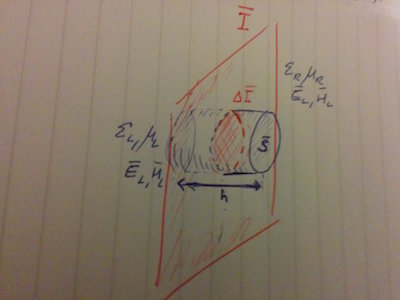
\includegraphics[height=0.3\textheight]{Figures/Chapters/PhysicalProblem/interfaceEPillBox}
  \end{center}
  \caption{Schematic showing integration surfaces used to obtain conditions for
    normal fields across an material interface.}
  \label{fig:material-interface-derivation:E-pillbox}
\end{figure}
In the limit $h \to 0$, all electric flux leaves the volume through the parallel
planes of the surface $S$, and~\eqref{eq:maxwell-gauss-integral} can be written
as
$$
\D_L \cdot \hat{\mathbf{n}} \Delta I - \mathbf{D}_R \cdot \hat{\mathbf{n}}
\Delta I = \rho_s \Delta I,
$$
where we have assumed that $S$ is sufficiently small that $D$ is constant. The
material interface condition can be written as
$$
\D_L \cdot \hat{\mathbf{n}} - \mathbf{D}_R \cdot \hat{\mathbf{n}} = \rho_s .
$$
Note that in the case where $\rho_s = 0$, meaning that there are no free
(unbound) charges, then the normal component of the electric flux density, $D$,
is continuous across the interface. By following the analogous procedure for the
magnetic field using~\eqref{eq:maxwell-gauss-magnetism-integral} we obtain
$$
\B_L \cdot \hat{\mathbf{n}} = \B_R \cdot \hat{\mathbf{n}} .
$$
These conditions are used with Maxwell's divergence equations.
% not used in the code!?

\subsection{Tangental fields}

Similarily for the tangental component of electric field we consider a closed
rectangular integration path in the plane of $\E_L$ and $\E_R$ around the same
interface, as shown
in~\eqref{fig:material-interface-derivation:E-rectangular-loop}. Again in the
limit $h \to 0$ and noting that $d\maxwellSource = 0$, we can
write~\eqref{eq:maxwell-faraday-integral} as
\begin{figure}[htbp!]
  \begin{center}
    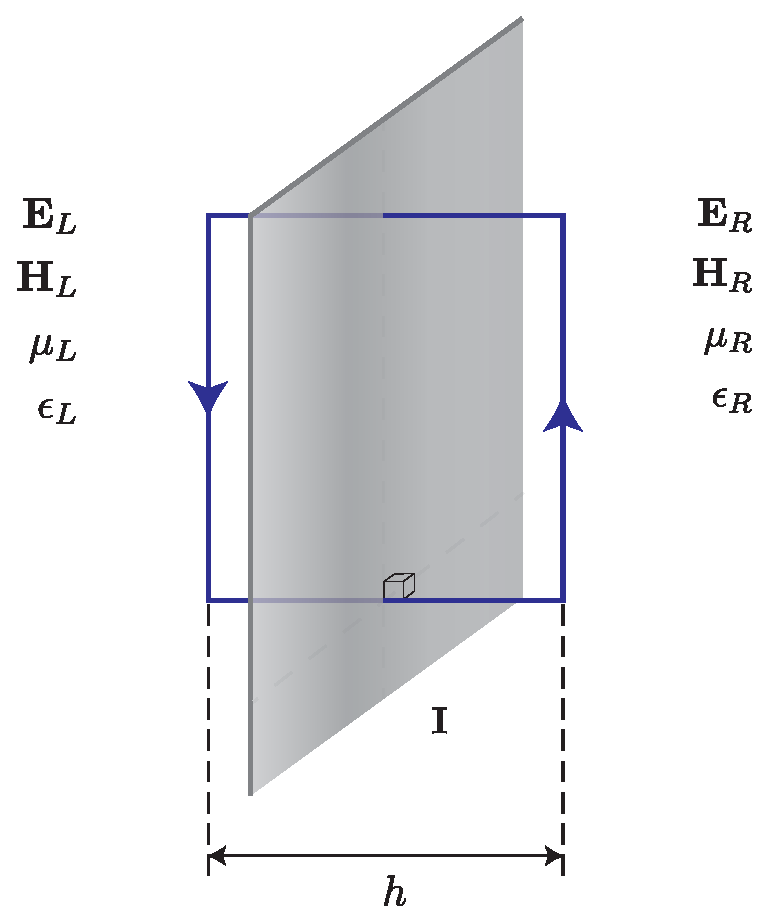
\includegraphics[height=0.3\textheight]{Figures/Chapters/PhysicalProblem/interfaceContour}
  \end{center}
  \caption{Schematic showing integration contours used to obtain conditions for
    tangental fields across an material interface.}
  \label{fig:material-interface-derivation:E-rectangular-loop}
\end{figure}
\begin{equation}
  \label{eq:material-interfaces-tangentalcondition-E}
  \int_{L_1}^{L_2} \E_L \cdot d\mathbf{l} - \int_{R_1}^{R_2} \E_R \cdot d \mathbf{l} = 0
\end{equation}
or
$$
\E_L \cdot d\mathbf{l} = \E_R \cdot d \mathbf{l} .
$$

The resulting interface condition is therefore that components of $\E$ tangental
to the interface are continuous - which can be written more generally as
$$
\hat{\mathbf{n}} \times \E_L = \hat{\mathbf{n}} \times \E_R .
$$
Again following an analogous procedure for the magnetic field we obtain
$$
\hat{\mathbf{n}} \cdot \H_L = \hat{\mathbf{n}} \times \H_R .
$$
These conditions are used with Maxwell's curl equations.

\subsection{Perfect electric conductors}
Metals with a large number of conduction band electrons can be described by the
perfect electric conductor (PEC) approximation. In a PEC the coulomb repulsion
between electrons causes all free charges to be distributed in an
infinitesimally thin layer on the surface of the material. The distribution of
free charges within a PEC changes instantaneously to counteract any applied
electric fields. Let us consider that the material on the right hand side of the
interface described above is a PEC. In this case, since $E_R$ is zero inside the
material, then~\eqref{eq:material-interfaces-tangentalcondition-E} simply
becomes
$$
\int_{L_1}^{L_2} \E_L \cdot d\mathbf{l} = 0 ,
$$
and the resulting condition is
$$
\E_L \times \hat{\mathbf{n}} = 0 .
$$
Similarily for the magnetic field we obtain
$$
\H_L \times \hat{\mathbf{n}} = \J_s ,
$$
% TODO - what about the other two conditions i.e. divergence conditions - should
% I specify those too?
where $\J_s$ is the surface current.

\subsection{Radiation condition}
Solution of many problems of interest require computation of phenomena occuring
in a physical domain of infinite extent. In such a domain, electromagnetic
sources should scatter energy to infinity. The inverse process, where radiation
transfers energy from infinity to location of the sources is non-physical. To
ensure uniqueness of solutions in an infinite domain, the following condition,
known as the Silver-M\"uller radiation condition, should be satisfied
\begin{align}
  \lim{ r \to \infty } \left( \xbf \times \left( \nabla \times \E \right) + \norm{\xbf} \dpartt{\E} \right) = 0, \\
  \lim{ r \to \infty } \left( \xbf \times \left( \nabla \times \H \right) + \norm{\xbf} \dpartt{\H} \right) = 0.
\end{align}

\section{Relation to wave equation and Helmholtz equation}
\subsection{Wave equation}

Within a homogenous medium, where material parameters are constant and no free
currents or charges are present, Maxwell's equations can be written in wave
equation form, for which plane wave analytical solutions can be
obtained\cite{Jackson:490457}. By combining Faraday's law in SI
form,~\eqref{eq:maxwell-ampere}, with the appropriate constitutive equations for
non-dispersive media,~\eqref{eq:constitutive-linear}, we obtain the expression
\begin{equation}
  \label{eq:wave-equation-derivation-1}
  \nabla \times ( \nabla \times \H ) + \eps_0 \eps_r \dpartt{ \nabla \times \E } = 0 .
\end{equation}
where in the absence of free currents and charges we have used $\J = 0$ and
$\rho = 0$.

Subsituting both the vector identity $ \nabla \times ( \nabla \times \H ) =
\nabla \cdot ( \nabla \cdot \H ) - \nabla^2 \H, $ where we note
from~\eqref{eq:maxwell-gauss-2} that $\nabla \cdot \H = 0$, and Ampere's
law,shown in~\eqref{eq:maxwell-ampere},
into~\eqref{eq:wave-equation-derivation-1} we obtain

\begin{equation}
  \label{eq:maxwell-wave-eqtn-H}
  \nabla^2 \H = \frac{1}{c^2} \ddpartt{ \H },
\end{equation}
which is a wave equation in the unknown $\H$, with the speed of the resultant
wave given by $c_0 = 1/\sqrt{\eps_0 \eps_r \mu_0 \mu_r }$. We note that the
quantities $\eps_0$ and $\mu_0$ are related to the speed of light in vacuum $c_0
= 1/\sqrt{\eps_0 \mu_0 }$. A similar procedure can be followed, starting from
Ampere's law, leading to
\begin{equation}
  \label{eq:maxwell-wave-eqtn-E}
  \nabla^2 \E = \frac{1}{c^2} \ddpartt{ \E } .
\end{equation}
% TODO - Ruben : comments are missing - what are the advantages/limitations of
% this formulation!! Look at LeVeque - why do we use conservation laws in this
% way?

\subsection{Helmholtz equation}
The Helmholtz or reduced wave equation form of~\eqref{eq:maxwell-wave-eqtn-E} is
of particular interest for frequency domain numerical simulations. In this
approach the fields $\E$ and $\H$ are assumed to be time-harmonic, and are
expressed as
\begin{align}
  \label{eq:maxwell-helmholtz-time-harmonic}
  \E(\xbf,t) = \Re \left( \EHelm(\xbf) e^{i \omega t} \right), \\
  \H(\xbf,t) = \Re \left( \HHelm(\xbf) e^{i \omega t} \right),
\end{align}

which, by substitution into the wave equations given
in~\eqref{eq:maxwell-wave-eqtn-E} and~\eqref{eq:maxwell-wave-eqtn-H} we obtain
the Helmholtz equations for electric and magnetic fields
\begin{align}
  \label{eq:helmholtz}
  \nabla^2 \E(\xbf) + k^2 \E(\xbf) = 0, \\
  \nabla^2 \H(\xbf) + k^2 \H(\xbf) = 0,
\end{align}
where $k^2 =\omega^2/c^2$, is known as the propagation constant.

In this form the equations for $\E$ and $\H$ can be solved independently for
each angular frequency, $\omega$. This approached is best suited to problems
with a small number of frequencies of interest, for example a system which is
being driven at a known frequency. By contrast time domain approaches allow
solution for a broad band of frequency responses at once.


% TODO Balanis citation is incomplete P Drude - needs to be removed - maybe the
% solid state one (Optical properties of solids) instead Maybe swap some of the
% references for others (e.g. Fox) Ruben made LOADS of comments on citations Use
% some citations from Rubens paper also


%%% Local Variables:
%%% mode: latex
%%% TeX-master: "../Thesis"
%%% End:

%% Chapter 1
\chapter{Numerical Method Review}
\label{NumericalMethodsChapter}
\lhead{Chapter 3. \emph{Numerical Method Review}}

Today there are several poular methods for solving maxwells equations. The one which remains in widespread use due to its simplicity and low operation count is the Yee Scheme \cite{YeeScheme} which uses a Finite Difference method. However the use of cartesian structured grids means that geometrical boundaries are subject to staircasing effects.

% jumping in too early with this...

Improved approximation of boundaries requires global refinement of the entire grid. It has been shown that small changes in the boundary representation for some electromagnetic problems can cause global changes in the solution \cite{RubenNEFEM}.

\subsection{Unstructured Mesh}
\begin{itemize}
  \item justify using FEM + limitations of FDTD
  \item unstructured mesh vs structured grid - stair-casing/geometric flexibility
  \item better represent boundaries with mesh refinement
  \item refine away from boundaries to capture solution not geometry
  \item hybrid meshes
\end{itemize}

Several techniques have been propsed to resolve these issues - notably the finite element and finite volume methods. These method allow the problem to be discretised on an unstructured mesh. One key advantage is that this allows local refinement near geometrical boundaries whilst still performing computations on a course mesh away from these boundaries. Refinement may also be used to capture the solution in regions where it is more complex without global refinement of the mesh.

However, a number of issues still remain with this approach. Boundaries are approximated by a linear approximation, which may include discontinuities in the boundaries or derivatives of the boundaries and can lead to non-physical effects []. Also the linear approximation of the solution means that these methods are subject to numerical disperion and dissipation which can cause significant errors in wave solutions propagated for long periods of time [].

\subsection{High Order FEM}
\begin{itemize}
	\item Capture geometric boundaries with elements with polynomial edges/faces
  \item interpolate soltn with polynomials
	\item still have non-physical effects due to inexact boundary representation - example global effect small change
	\item options for high order (FEM)
  \item numerical dispersion/dissipation - problem for long propagation
  \item limitations: sparse + global matrix, geometry representation, parallelisation
\end{itemize}

High-order methods allow boundaries to be approximated with polynomials by allowing elements to have curved faces - which greatly reduces staircasing effects []. Additionally the solution if approximated with a polynomial basis, whose order can be changed per element for local refinement. Higher order shape function have been shown to reduce dispersion and dissipation effects and allows, for smooth solutions, an improved accuracy for the same number of degrees of freedom. However this results in a sparse global mass matrix which needs to be inverted at each time step to solve the problem. This can be be very computationally expensive both in terms of CPU time required to invert the matrix and memory requirements.

Additionally for applications discussed in this thesis a long-running simulations are required [Chapter reference], therefore a method which can be parallelized would be desirable.

\subsection{Advantages Of Discontinuous Galerkin}

\begin{itemize}
  \item introduce method
	\item how does DG address the issues with FEM
  \item advantages for wave-dominated problems
	\item Capturing wave solutions + numerical dissipation/dispersion
	\item Influence of numerical flux
\end{itemize}

The Discontinuous Galerkin method uses a high-order polynomial basis for shape functions and and unstructured mesh - which for accurate approimation of boundaries. The method introduces additional degrees of freedom when compared with the finite element method, however this results in a block diagonal mass matrix, which can easily be inverted. Additionally the block diagonal structure means that computation can be distributed between a number of processors and performed in parallel.

% can I change p in different elements in normal finite element....?


% -------------
  

%The linear approximation of boundaries in low-order schemes has been shown to cause non-physical issues with the solution as a whole []. These low-order approximations of boundaries can include discontinuities in the boundaries themselves or derivaties of the boundaries (staircasing) which can lead to non-physical effects. High-order schemes allow us to approximate boundaries and interfaces with polynomials.

% \begin{itemize}
% \item Finite Difference, Finite Volume, Finite Element, Other High Order competitors to DG
% \end{itemize}
  
% OPTIONS LEFT: FINITE DIFFERENCE, FINITE VOLUME, FINITE ELEMENT
% Finite difference schemes seem very promising and are very popular however in many cases these have many limitations. In FDTD the entire computational domain is discretized using a cartesian structured grid. Complex geometrical boundaries or interfaces become hard to capture with structured grids - and improving the approximation of the boundary requires refiniment of the entire grid. Furthermore capturing solutions which are more complex in certain regions again require refinement over the whole domain. Clearly methods which use an unstructured mesh have a clear advantage since the geometry can be captured accurately with only local refinement of the mesh.

% OPTIONS LEFT: FINITE VOLUME (or other low order meshes), FINITE ELEMENT


% OPTIONS LEFT: FINITE ELEMENT (HIGH-ORDER)
% High-order FEM scheme have several issues having a sparse global matrix which needs to be inverted. The Discontinuous Galerkin method on the other hand has elemental matricies with elements connected by a numerical flux term. This means there are no large global matricies to invert. Also the approximations in high order are better however geometries are approximated by polynomials. This can still cause issues capturing geometries with a high curvature.


%The Discontinuous Galerkin method was first introduced in 1973 by Reed and Hill [W.H. Reed, T.R. Hill, Triangular mesh methods for the neutron transport equation, Los Alamos Scientific Laboratory, 1973 Tech. Rep. LA-UR-73-479] to solve the neutron transport equation.
%\chapter{Discontinuous Galerkin for Maxwells Equations} % Write in your own chapter title
\label{Chapter3}
\lhead{Chapter 3. \emph{Discontinuous Galerkin}} % Write in your own chapter title to set the page header

\subsection{Formulation}

The Discontinuous Galerkin method was first introduced to solve the neutron transport problem by Reed and Hill \cite{} in 1973.

** Some background/literature review here Cockburn, Shui for solving hyperbolic equations etc ***
% PhDJesusAlvarez good for motivation - not so much for the method

As seen in Chapter \ref{PhysicalProblemChapter}, given a suitable choice of initial conditions the evolution of the system in time can be described by Maxwell's curl equations \eqref{maxwell-curl-equations-conservation-form}, given again for convenience

$$
\ut + \fk  = \mathbf{S(U)}
\label{strong-form-DG}
$$

Consider that the problem is defined on a physical domain, $\Omega$, which can be discretised by an unstructured mesh of $K$ element such that

\begin{equation}
  \Omega \approx \Omega_h = \mathop{\bigcup}_{k=1}^{K} \Omega_e^k
\end{equation}
where $\Omega_e^k$ are the elements in the discretisation.  

% discuss the discretisation more - discontinuous elements etc

Following the method of weighted residuals the \eqref{strong-form-DG} is multiplied by a vector of test functions $\mathbf{W}$ and integrated over an element $\Omega_e^k$. The following weak form is obtained by integration by parts

$$
\int_{\Omega_e^k} \mathbf{W} \ut d\Omega_e^k  - \int_{\Omega_e^k} \frac{\partial \mathbf{W}}{ \partial x_k} \mathbf{F}_k(\mathbf{U}) d\Omega + \int_{\partial \Omega_e^k} \mathbf{W} \cdot \mathbf{F_n}(\mathbf{U_e}) d\Gamma = \int_{\Omega_e^k} \mathbf{W} \cdot \mathbf{S}(\mathbf{U_e}) d\Omega
\label{maxwell-DG-weak-form}
$$

where $n_k$ is the $k$th component of the element outward normal to $\partial \Omega_e^k$ and $\mathbf{F_n}$, the normal flux, is given by

$$
\mathbf{F_n}(\mathbf{U}) = \mathbf{F}_k(\mathbf{U}) n_k
$$

This weak form is specified on an element, however this is not yet a scheme suitable for solving the global problem. In order to recover the global solution the continuity of the solution between elements is weakly enforced by replacing the physical normal flux $\mathbf{F_n}(\mathbf{U_e})$ with a consistent numerical flux $\mathbf{\tilde{F}}_n(\mathbf{U}_e,\mathbf{U}_e^{out})$, evaluated in terms of the solution on an element, $\mathbf{U}_e$, and the is the value of the solution along a given face in adjoining element sharing that face, $\mathbf{U}^{out}$.

*** conditions to be satisfied by numerical flux + form of numerical flux ***

The system is discretised by choosing the solution approximated by
$$
U_e \simeq \sum_{i=1}^{n} u_{i} N_{i}
$$
where $N_{i}$ are Lagrangian shape functions and $u_{i}$ are nodal solution values. Following the Galerkin method test functions $W$ are then chosen with the same basis of shape functions:

$$
W = \sum_{i=1}^{n} N_{i}
$$

The resulting discretised system of equations can be written as a system of ordinary differentail equations

$$
\mathbf{M} \frac{d \mathbf{U}} {dt} + \mathbf{R}(\mathbf{U}) = 0
$$

where $\mathbf{U}$ is a vector of the coefficients $u_{i}$, $M$ is the mass matrix which is block diagonal and $\mathbf{R}$ is the residual vector.

*** RK4 Stability condition

\subsubsection{Local Element Equations}
\begin{itemize}
  \item problem in conservation form -> GMWR -> weak form
  \item discretised versions of relevant maxwells equations
	\item local matrix + broken space
	\item Nodal (or Modal) representation
\end{itemize}
\subsubsection{Numerical Flux}

\begin{itemize}
	\item recover solution with numerical flux
  \item numerical flux used
	\item upwind flux: effect for wave domination problems - flow of information, upwind flux
\end{itemize}

\subsection{Time Integration}
\begin{itemize}
	\item explicit RK4
	\item breif mention explicit justification in terms of delta t limit (and refer to chapter)
	\item justify high-order time integration
\end{itemize}

The solution is advanced in time with an explicit fourth order Runge-Kutta (RK4) method. Implicit schemes which allow larger time steps may be employed to solve the system of equations in a shorter computational time. However as detailed in section [ ***section ref *** ] the transient system behaviour at closely spaced intervals is required in order to reduce the accuracy in time. Thus an upper limit on timestep length is imposed by the frequencies of interest and the computation accuracy required.

\subsection{Implementing Boundary Conditions}
\begin{itemize}
	\item material interfaces (PEC,ABC)
  \item will need to mention PML -> another section
\end{itemize}

For interfaces which intersect the domain boundary, $\partial \Omega$, the not all components of $\mathbf{U}^{out}$ are determined by the boundary conditions on the interface. For a system of conservation laws Rankine-Hugoniot jump conditions of the form

$$
\left[[ \mathbf{F}_n \right]] = \lambda_j \left[[ \mathbf{U} \right]]
$$

where $\lambda_j$ are the eigenvalues of the jacobian matrix $\mathbf{A}_n$. For the 3-dimensional case

$$
\lambda_1 = \lambda_2 = \frac{1}{\sqrt{\epsilon_L \mu_L}}
$$

$$
\lambda_3 = \lambda_4 = 0
$$

and

$$
\lambda_5 = \lambda_6 = \frac{1}{\epsilon_R \mu_R}
$$
where the subscripts  $L$ and $R$ on the material parameters $\epsilon$ and $\mu$ denote the left and right side of the interface respectively.

are applied at the interfaces

\subsubsection{Spatial Discretisation}
\begin{itemize}
	\item discuss types of element - (non-)affine, planar, different shapes etc.
	\item condition number of a matrix - moving nodes around %reference!
\end{itemize}

\subsection{Errors and convergence}
\begin{itemize}
  \item expected rates of convergence for time-domain (interpolation error) and freq domain (dispersion error)
\end{itemize}

%
%-- Simulation  --
%
%PCB VCSEL
%
%-- Dispersive Photonic Crystals --
%* Photonic Crystal Vertical Cavity Surface Emitting Lasers -> 3 weeks
%  * Photonic Band-Gap Defect cavity - single cell
%  * Photonic Band-Gap hexagonal, square and stick waveguide resonators
%* Add-drop photonic band gap filters  -> 3 weeks
%  - square, circular, hex shapes
%  - double
%  - with/without "scatterers"
%* maybe a comparison to FDTD again -> 2 weeks
%
%-- 2D Examples --
%* Rectangular cavity with convergence curves (write up) -> done
%* PEC Circle cavity - comparison of NEFEM and high-order -> 2 week
%* Equilateral triangle cavity (or polygon) -> 1 week
%* Infinite 2D dielectric circle cavity (in a PML) with add-drop filter - Niegemann -> 2 weeks
%* Cylindrically symmetric cavity example (Bangor example) -> 2 weeks
% 
%-- Parallel Examples --
%* Aeroplane Scattering (comparison to low-order code) - might require some optimisations (faces etc) -> 2 weeks
%* Comparison of code speed for large 3D meshes -> 1 week
%* Study of partitioning for element orders and types (2D + 3D) -> 2 weeks


\label{Chapter3}
\chapter{Free space rectangular PEC cavity} % Write in your own chapter title

\begin{itemize}
  \item Problem setup
  \item Convergence of error with simulation period
  \item dt study
  \item Scheme convergence results
\end{itemize}

In this chapter we validate our results using a 2-dimensional rectangular free space ($\epsilon=\mu=1$) cavity of dimensions $a \times b$. Discrete resonant frequencies of the system are given by

$$
f_{nm} = \frac{1}{2 \pi \sqrt{\epsilon_r \mu_r}} \sqrt{ k_x^2 + k_y^2 }
$$
$$
k_{x} = \frac{m \pi}{a}^2
k_{y} = \frac{n \pi}{b}^2
$$

where $n$ and $m$ are the mode numbers.

\section{Time Domain Signals}

\figHere{Chapters/Results/2D_FreeSpaceCavity/signal/p1_signal}{The signal obtained for the $E_1$ component using $p=1$ and a mesh of 4 and 8 quadrilaterals}{2DPECCavityFreqConv}
\figHere{Chapters/Results/2D_FreeSpaceCavity/signal/p3_signal}{The signal obtained for the $E_1$ component using $p=3$ and a mesh of 8 and 128 quadrilaterals. Signal can be seeon to contain a higher frequency content than p1 signals.}{2DPECCavityFreqConv}
\section{Spectra}
Spectra for comparison of $p=1$ and $p=3$ for small (1x2) and large (8x16) meshes.
\figHere{Chapters/Results/2D_FreeSpaceCavity/spectrum/spectrum_1x2_p1}{The spectrum obtained for the TE mode using $p=1$ and a mesh of 1x2 quadrilaterals}{2DPECCavityFreqConv}
\figHere{Chapters/Results/2D_FreeSpaceCavity/spectrum/spectrum_2x4_p1}{The spectrum obtained for the TE mode using $p=1$ and a mesh of 2x4 quadrilaterals}{2DPECCavityFreqConv}
\figHere{Chapters/Results/2D_FreeSpaceCavity/spectrum/spectrum_2x4_p3}{The spectrum obtained for the TE mode using $p=3$ and a mesh of 2x4 quadrilaterals}{2DPECCavityFreqConv}
\figHere{Chapters/Results/2D_FreeSpaceCavity/spectrum/spectrum_8x16_p3}{The spectrum obtained for the TE mode using $p=3$ and a mesh of 8x16 quadrilaterals}{2DPECCavityFreqConv}

\clearpage
\subsection{h-Convergence of Frequency}
Figure \ref{2DPECCavityFreqConv} shows the convergence of frequency obtained for a cavity with $a=0.5$ and $b=1.0$ for three differents meshes of quadrilateral elements.
%% NOTE::: HAVE I TRIED THIS WITH TRIANGLES

\figHere{Chapters/Results/2D_FreeSpaceCavity/freqConvergence/U2F1}{The convergence of absolute error in the frequency is shown for three different meshes using shape functions of order 1,2 and 3}{2DPECCavityFreqConv}
\figHere{Chapters/Results/2D_FreeSpaceCavity/periodConvergence/U2F1}{Convergence of absolute error in the frequency with the final time, $T$, of the simulation for a number of meshes and $p$ for \textbf{Frequency 1} for a rectangular PEC cavity}{2DPECCavityFreqConv}
\figHere{Chapters/Results/2D_FreeSpaceCavity/freqConvergence/U2F2}{The convergence of absolute error in the frequency is shown for three different meshes using shape functions of order 1,2 and 3}{2DPECCavityFreqConv}
\figHere{Chapters/Results/2D_FreeSpaceCavity/periodConvergence/U2F2}{Convergence of absol    ute error in the frequency with the final time, $T$, of the simulation for a number of     meshes and $p$ for \textbf{Frequency 2} for a rectangular PEC cavity}{2DPECCavityFreqConv}
\figHere{Chapters/Results/2D_FreeSpaceCavity/freqConvergence/U2F3}{The convergence of absolute error in the frequency is shown for three different meshes using shape functions of order 1,2 and 3}{2DPECCavityFreqConv}
\figHere{Chapters/Results/2D_FreeSpaceCavity/periodConvergence/U2F3}{Convergence of absol    ute error in the frequency with the final time, $T$, of the simulation for a number of     meshes and $p$ for \textbf{Frequency 3} for a rectangular PEC cavity}{2DPECCavityFreqConv}
\clearpage
\figHere{Chapters/Results/2D_FreeSpaceCavity/freqConvergence/U2F4}{The convergence of absolute error in the frequency is shown for three different meshes using shape functions of order 1,2 and 3}{2DPECCavityFreqConv}
\figHere{Chapters/Results/2D_FreeSpaceCavity/periodConvergence/U2F4}{Convergence of absol    ute error in the frequency with the final time, $T$, of the simulation for a number of     meshes and $p$ for \textbf{Frequency 4} for a rectangular PEC cavity}{2DPECCavityFreqConv}
\figHere{Chapters/Results/2D_FreeSpaceCavity/freqConvergence/U2F5}{The convergence of absolute error in the frequency is shown for three different meshes using shape functions of order 1,2 and 3}{2DPECCavityFreqConv}
\figHere{Chapters/Results/2D_FreeSpaceCavity/periodConvergence/U2F5}{Convergence of absol    ute error in the frequency with the final time, $T$, of the simulation for a number of     meshes and $p$ for \textbf{Frequency 5} for a rectangular PEC cavity}{2DPECCavityFreqConv}
\figHere{Chapters/Results/2D_FreeSpaceCavity/freqConvergence/U2F6}{The convergence of absolute error in the frequency is shown for three different meshes using shape functions of order 1,2 and 3}{2DPECCavityFreqConv}
\figHere{Chapters/Results/2D_FreeSpaceCavity/periodConvergence/U2F6}{Convergence of absol    ute error in the frequency with the final time, $T$, of the simulation for a number of     meshes and $p$ for \textbf{Frequency 6} for a rectangular PEC cavity}{2DPECCavityFreqConv}
\clearpage
\figHere{Chapters/Results/2D_FreeSpaceCavity/freqConvergence/U2F7}{The convergence of absolute error in the frequency is shown for three different meshes using shape functions of order 1,2 and 3}{2DPECCavityFreqConv}
\figHere{Chapters/Results/2D_FreeSpaceCavity/periodConvergence/U2F7}{Convergence of absol    ute error in the frequency with the final time, $T$, of the simulation for a number of     meshes and $p$ for \textbf{Frequency 7} for a rectangular PEC cavity}{2DPECCavityFreqConv}
\figHere{Chapters/Results/2D_FreeSpaceCavity/freqConvergence/U2F8}{The convergence of absolute error in the frequency is shown for three different meshes using shape functions of order 1,2 and 3}{2DPECCavityFreqConv}
\figHere{Chapters/Results/2D_FreeSpaceCavity/periodConvergence/U2F8}{Convergence of absol    ute error in the frequency with the final time, $T$, of the simulation for a number of     meshes and $p$ for \textbf{Frequency 8} for a rectangular PEC cavity}{2DPECCavityFreqConv}
\figHere{Chapters/Results/2D_FreeSpaceCavity/freqConvergence/U2F9}{The convergence of absolute error in the frequency is shown for three different meshes using shape functions of order 1,2 and 3}{2DPECCavityFreqConv}
\figHere{Chapters/Results/2D_FreeSpaceCavity/periodConvergence/U2F9}{Convergence of absol    ute error in the frequency with the final time, $T$, of the simulation for a number of     meshes and $p$ for \textbf{Frequency 9} for a rectangular PEC cavity}{2DPECCavityFreqConv}
\clearpage
\section{p3 Convergence Comparison}
4 runs have been performed for different meshes with $p=3$

Run 1 =  monitor at [ -1, 0.5 ] ctt=0.45.

Runs 2 + 3 = monitor at [ 0.5,0.5] ctt=0.1 (different final times).

Run 4 = mointor at [ 0.5,0.5 ] ctt=0.4

Error due to determining the peak?

\figHere{Chapters/Results/2D_FreeSpaceCavity/convergenceComparisonP3/ConvergenceforU2F5}{Convergence with p3 only - h=1.2 not converged for this frequency, but h=0.9 is}{label}
\figHere{Chapters/Results/2D_FreeSpaceCavity/convergenceComparisonP3/ConvergenceforU2F6}{Convergence with p3 only - h=1.2 not converged for this frequency, but h=0.9 is}{label}
\figHere{Chapters/Results/2D_FreeSpaceCavity/convergenceComparisonP3/ConvergenceforU2F7}{Convergence with p3 only - h=1.2 may not be converged}{label}
\figHere{Chapters/Results/2D_FreeSpaceCavity/convergenceComparisonP3/ConvergenceforU2F8}{Convergence with p3 only - h=1.2 may not be converged}{label}
\figHere{Chapters/Results/2D_FreeSpaceCavity/convergenceComparisonP3/ConvergenceforU2F9}{Convergence with p3 only - h=1.2 may not be converged}{label}
\figHere{Chapters/Results/2D_FreeSpaceCavity/convergenceComparisonP3/ConvergenceforU2F10}{Convergence with p3 only - h=1.2 may not be converged}{label}


\label{Chapter3}
\chapter{Free space circular PEC cavity} % Write in your own chapter title

\begin{itemize}
  \item Problem setup
  \item Convergence of error with simulation period
  \item dt study
  \item Scheme convergence results
\end{itemize}

In this chapter we validate our results using a 2-dimensional rectangular free space ($\epsilon=\mu=1$) cavity of dimensions $a \times b$. Discrete resonant frequencies of the system are given by

$$
f{nm} = \frac{1}{2 \pi \sqrt{\epsilon_r \mu_r}} k_{mp}
$$

$$
k_{mp}=\sqrt{ k_x^2 + k_y^2 }
$$
$$
k_{x} = \frac{m \pi}{a}^2
k_{y} = \frac{n \pi}{b}^2
$$

where $n$ and $m$ are the mode numbers.

\subsection{Spectra}
\figHere{Chapters/Results/2D_FreeSpacePECCircle/spectrums/U1}{Spectrum for $E_1$ component with $p=1$ elements with planar edges for different mesh refinements}{2DPECCavityFreqConv}
\subsection{h-Convergence of frequency}
Figure \ref{2DPECCavityFreqConv} shows the convergence of frequency obtained for a cavity with $a=0.5$ and $b=1.0$ for three differents meshes of quadrilateral elements.
%% NOTE::: HAVE I TRIED THIS WITH TRIANGLES

\figHere{Chapters/Results/2D_FreeSpacePECCircle/hConvergencePlots/combined}{Convergence of absolute error in the frequency with characteristic mesh size using exact geometry representation and planar faced elements with $p=1$ for a PEC circle. The expected gradient of 4 is obtained with the NEFEM mesh and a gradient of 2 is obtained with FEM.}{2DPECCavityFreqConv}

\figHere{Chapters/Results/2D_FreeSpacePECCircle/convPlotsAll/convAll_iComp2}{Convergence of absolute error in the frequency with p-refinement using NEFEM, planar edges and curved edge elements}{2DPECCavityFreqConv}

\figHere{Chapters/Results/2D_FreeSpacePECCircle/ndofConvergencePlots/p_vs_h_ndof/eps/F4} {Convergence of error in the frequency with number of degrees of freedom comparison between h-refinement with planar elements and p-refinement for a PEC circle. Both types of refinement are shown both with exact geometry representation and with curved high-order elements.}{2DPECCavityFreqConv}


\chapter{Dispersive 2D Cavity} % Write in your own chapter title
\label{Chapter3}
\lhead{Chapter 3. \emph{Dispersive 2D Cavity}} % Write in your own chapter title to set the page header

\begin{itemize}
	\item set up problem with volumetric source
	\item show convergence of wave shapes
\end{itemize}

\section{h-convergence with volumetric source}
\figHere{Chapters/Results/2D_DispersivePlate/convergenceAllComponents/eps/L2vsH_TE_single_comp}{L2 Norm convergence in time domain waveform for TE mode of dispersive plate}{label}
\figHere{Chapters/Results/2D_DispersivePlate/convergenceAllComponents/eps/L2vsH_TM_single_comp}{L2 Norm convergence in time domain waveform for TM mode of dispersive plate}{label}

\section{h-Convergence with frequency}

\chapter{3D Cube PEC Example} % Write in your own chapter title
\label{Chapter3}
\lhead{Chapter 3. \emph{3D Cube Example}} % Write in your own chapter title to set the page header

\figHere{Chapters/Results/3D_Cube/spectrums/spectrum_p3_HEX_H3}{Spectrum for $p=3$ H3 with hexahedral elements showing a component of $E$ and $H$}{2DPECCavityFreqConv}

\figHere{Chapters/Results/3D_Cube/convPlotsAll/HEXConvergenceforU1F2}{Hex convergence for $E_1$}{label}
\figHere{Chapters/Results/3D_Cube/convPlotsAll/HEXConvergenceforU1F5}{Hex convergence for $E_1$}{label}
\figHere{Chapters/Results/3D_Cube/convPlotsAll/HEXConvergenceforU1F6}{Hex convergence for $E_1$}{label}
\figHere{Chapters/Results/3D_Cube/convPlotsAll/HEXConvergenceforU1F7}{Hex convergence for $E_1$}{label}
\figHere{Chapters/Results/3D_Cube/convPlotsAll/HEXConvergenceforU1F8}{Hex convergence for $E_1$}{label}
\figHere{Chapters/Results/3D_Cube/convPlotsAll/HEXConvergenceforU1F9}{Hex convergence for $E_1$}{label}

\figHere{Chapters/Results/3D_Cube/convPlotsAll/TETConvergenceforU1F2}{Tet convergence for $E_1$}{label}
\figHere{Chapters/Results/3D_Cube/convPlotsAll/TETConvergenceforU1F5}{Tet convergence for $E_1$}{label}
\figHere{Chapters/Results/3D_Cube/convPlotsAll/TETConvergenceforU1F6}{Tet convergence for $E_1$}{label}
\figHere{Chapters/Results/3D_Cube/convPlotsAll/TETConvergenceforU1F7}{Tet convergence for $E_1$}{label}
\figHere{Chapters/Results/3D_Cube/convPlotsAll/TETConvergenceforU1F8}{Tet convergence for $E_1$}{label}
\figHere{Chapters/Results/3D_Cube/convPlotsAll/TETConvergenceforU1F9}{Tet convergence for $E_1$}{label}

Parallel: benchmark times for communication and calculation for different meshes + compare to overall performance plots should appear somewhere - should appear somewhere in results.

%\label{Chapter5}
\chapter{Parallelisation} % Write in your own chapter title
\lhead{Chapter 5. \emph{Parallelisation}} % Write in your own chapter title to set the page header

[[ Introduction goes here ]]
The weak form of Maxwells equations means that parallelisation strategies are possibile.

The Message Passing Interface (MPI) is used and a *** strategy with distributed memory is utilised. The parallel computation is performed by a process of data decomposition. This means that the computational domain is partitioned into regions of space and each processor performs computations only on the elements in that region. This is made possible by the form of the weak form given in \eqref{maxwell-DG-weak-form}. We note that the weak form involves primarily values of unknowns on a single element. The only exception being the values of the solution $U_{out}$ from neighbouring elements required for the calculation of the numerical flux, $\tilde{\mathbf{F}}_n$ along element faces. These values should be made available to each element by communication between processors at each timestep.

\section{Update Equations in Parallel}
Consider an open bounded domain $\Omega \subset \R^{n}$ with boundary $\partial \Omega$ where the boundary, $\partial \Omega = \Gamma^{PEC} \cup \Gamma^{ABC}$, is composed of segments, $\Gamma^{PEC}$, along which PEC boundary condition are prescribed and segments, $\Gamma^{ABC}$, along which ABC boundary conditions are prescribed which satisfy $\Gamma^{PEC} \cap \Gamma^{ABC} = \O$. We define the internal faces of the domain as $\Gamma^{I} = ( \cup_e \partial \Omega_{e}) \setminus \partial \Omega$.

, partitioned with a regular partitioning in the usual way for finite elements as $\bar{\Omega} = \cup_{e} \bar{\Omega}_e$, such that $\Omega_i \cap􏰰\Omega_j = \O$, for $i \ne j$. 

We wish to divide the computational load between processors, by assigning calculations of each element to different processors. We define a regular partioning of $\Omega$ as $\bar{\Omega} = \cup_{p} \bar{\Omega}^p$ with partition boundary $\partial \Omega^{p}$. Each non-overlapping partition $\Omega^p$ is composed of a number of elements such that $\bar{\Omega}^p = \cup_{e} \bar{\Omega}_e$ and $\Omega^i \cap \Omega^j = \O$, for $i \ne j$. Let us consider calculation of updated solution values, $U^{n+1}_i$, from solution values at the previous timestep, $U^{n}_i$ for an element $\Omega_i$. We achieve parallelisation by assigning computation of the values $U^{n+1}_i$ from $U^{n}$ for each element $\Omega_e \in \Omega^p$ to a processor $P^p$. 

For an element $\Omega_e \in \Omega^p$ we can define its adjacent elements, that is elements that share a face or edge, as $A_e = \{ \Omega_a \subset \Omega \| \partial \bar{\Omega}_a \cap \partial \bar{\Omega_e} \ne \O \}$. In general $A_e$ is composed of internal adjacent elements, $A_e^{int} = \{ A_e \cap \Omega^p \}$ , and external adjacent elements, $A_e^{ext} = \{ A_e \cap \Omega \setminus \Omega^p \}$. If $A_e^{ext} = \O$ the element $\Omega_e \in \Omega^p$ is said to be an internal element of $P^p$, and when $A_e{ext} \ne \O$ is said to be an interface element of $P^p$.An element $\Omega_e \in \Omega \setminus \Omega^p$ is said to be an external element of $P^p$.


Each element requires nodal values of $U_i^{n}$ from each of its adjacent elements only along shared faces (or edges). However in order to simplify the implementation, all nodal values of the solution of adjacent elements is communicated to the element in question at every time step. In this case the same data structures and conventions as outlined in Chapter [***] can be used to store the nodal values from other processors - which simplifies treatment in the code. This will incur a small performance penalty, however, for two processors containing a single triangle each with planar edges and linear shape functions communication was found to be only **** percent of total calculation time. This is expected to be an extreme case where computation greatly exceeds calculation time. However more realistic systems such as **** communication was only *** percent.

If the element $\Omega_e \in \Omega^p$ is an internal elements of $P^p$ all of the values of $U_i^n$ required to calculate $U_i^{n+1}$ are available on the processor $P^p$ from calculations on the previous timestep. However, if $\Omega_e$ is an interface elements, some of the values of $U_i^{n}$ will be available from calculations on $P^p$ for elements $A_e^{int}$, but will have been calculated on another processor on $A_e^{ext}$. At each time step, prior to face calculations, values of $U_i^{n}$ for elements in $A_e^{int}$ will be required on $P^p$, and should be sent to by each processor to which any element in $A_e^{int}$ is assigned. Or conversely, for each interface element, $\Omega_i$ in processor $P^p$, updated values of $U_n^i$ should be sent to any processors containing any element in $A_e^{ext}$.

% maybe define what an adjacent processor of an ELEMENT is - that could help
% mention when U_out need to be available? Prior to compution. U_out calc prev time step.
% I've not mentioned (really) any correspondence between L^p_{out} and L^p_{in}
% talk about types of these elements and illustrate further with examples (figures)
% this could also be done as \Omega_i \subset L^p_{out} ?? How to I say that 

\section{Domain decomposition}

%% [ *** AT SOME POINT I SHOULD MENTION THAT THE T (and element type info) IS READ FROM THE MESH ]

Since communication is an expensive operation with a significant overhead associated with each connection established we wish to minimise both the number of connections established and the information communicated at each time step. The number of messages can be significantly reduced by sending all values of $U_{n}$ once at the end of each time step.
% how much overhead? How expensive? What is more important? Communication of Computation?
Additionally we wish to choose $\Omega^p$ such that we minimise the number of processors which are required to communicate with each other, the volume of data which needs to be sent and the number of connections which needs to be established.
% *** is the number of connections ACTUALLY a different thing?
% *** at a later date I could also minimise the number of unknowns to communicate by weightng ( that comes under volume of data)


The three criteria can be met, if all elements have the same number of unknowns, by minimising the total number of external adjacent elements of all elements. This is equivalent to minimising the number of faces with in which the elements are on different processors. This operation can be performed by the public-domain library parMETIS [***], which implements several algorithms for the optimal partitionining of graphs.

% other processor has to know who they're from!! Talk about this in implementation
faces)
The parMETIS library requires a graph of the connectivities of all elements, in which each node of the graph represents an element and each edge of the graph represents a face shared between two elements. Since partitioning of the graph is performed in parallel the graph is given in a distributed data format in which each processor contains only a subset of the graph defined by a range of element indicies. The parMETIS library the accepts as a first parameter which specifies these ranges as an array which specifies for each processor the the first element index in its range. The last element index is then the element before the first element assigned to the next processor. The elements were distributed between processors equally, and the global element numbering established in the mesh file was used as a common numbering scheme between processors without need of communication.
A more optimal partitioning could be achieved if required by considering the type of each element and therefore the maximum number of shared faces, this however would require communication between processors in order to establish a common element indexing which is sequential within each processor. This would add significant to the complexity to the code and was not required for the problems which were considered.
% [*** not start points ? *** ]

The vertices of the graph are obtained by first constructing a node connectivity list, which for each node lists the elements which contain that node. This list is constructed by reading the whole mesh connectivity information and associating each read element which all the nodes it contains. The connectivites for all elements is read - however since these are integer values memory usage is not considered relevant [ *** give an example of a very large mesh]. We loop through all faces of the elements allocated to this processor and for each face perform a loop on the nodes within that face. Within the inner loop we construct a list of connected elements [what is this]. The connected face will be the element in this list which appears the same number of times as the number of nodes in the face.

From the connectivity graph, parMETIS can then optimise the partitions in such a way to reduce the number of faces shared across processors. The resulting partition is shown for a circle with 5 processors in \figref{parmetis-figure}

The result of the optimisation by parMETIS is a list of all elements allocated to this processor and a number between 1 and the total number of processors (or equivalently the number of parts into which the domain is partitioned) which indicated the processor on which calculations should be performed (or equivalently the parition in which this element belongs). We allow each partition of the domain to correspond to a partitioning $\Omega^p$.

\section{Communication Arrays and Data Partition}

Recall that in order to implement the parallelised DG method it is not sufficient to distribute computations, some values of solution need to be communicated at each time step. In order to simplify the extension of a serial code to multiple processors the strategy employed involves establishing the set of elements that, for a given processor $A$, share a face with an element in the partition allocated to processor $A$. All nodal solution values for these elements are mirrored from the processor on which they are calculated to processor $A$ at each time step. The data partition is show in \figref{parmetis-figure} and results in a number local elements on which calculations are performed on this processor and a number of interface elements for which nodal solution values are available without calculation. By this data partition method code to calculate the numerical flux contributions does not need to distinguish betweeen local elements and interface elements. The advantage of this method is that the elements allocated to a processor and the interface elements can be stored in the same data structures.

Once the partitioning has been performed parMETIS provides a list of partition numbers, the length of the number of elements in the partition range of this processor. The partition numbers correspond to the processor partition $\Omega^p$, to which the given element should be allocated for calculation. In order to set up communication arrays additional information is required. For each element allocated to a partition $P$ the elements to which it is connected are required, which is available on the current partition, and also a list of the processors on which the element will the allocated for calculation. These eventual destinations are obtained for each element by MPI communication following partitioning. Then for each element the global index of the element and a list of the global indexes of its adjacent elements which are not on the destination processor and for each of those adjacent elements the processor on which they will be located is sent to the processor on which communication will occur.

Each processor will therefore recieve from all processors a list of the elements that are allocated to that processor and also a list of the elements to which those elements are connected. Note that in this instance the processor is sending information to itself via MPI, but this will not incur a communication overhead. From this information a list of all the elements on this processors for which calculations will occur, or local elements, can be constructed and also a list of all elements which are connected by a shared face one or more times to this processor, the non-local elements. The mesh connectivity information can then be re-read for all elements (both local and non-local) and coordinates of mesh vertices are required for local elements. The code may then proceed exactly as in the serial case but only looping over the local elements for calculations. The only difference is that following each solution update communication should occur to update the nodal in the interface elements based on the elements in the other processor.

Now each processor knows it local elements, its non-local elements and for each non-local element it knows the processor on which those non-local element are calculated. I also (should know) for each element calculated on this processor the list of destination processors to which the element should be sent. A list is created on each processor in processor order (i.e. one processor at a time) of elements to send to the processors and this list is done (by processor) in global element index order. Provided that each processor stores the data for its (unique) non-local elements in global element index order by the processor on which the calculation occurs then a single call to MPI\textunderscore SEND \textunderscore TO \textunderscore ALL operation can directly populate the non-local element data. The only additional operation required is to create a the buffers for the send will not necessarily to bein contiguous memeory therefore on each processor a temporary buffer must be available to which the element data of all elements is written contiguously prior to send.

*** The mesh can then be re-read for all local elements and element types are required for non-local elements. This will involve renumbering the elements and introducing a new uniuque local element and node numbering in order to maintain a continuous local node indexing.

% QUESTION: should I keep track of localElementMap after preprocess? maybe for output?

\section{Communication Arrays and Data Partition}

\begin{figure}[htbp!]
 \centering
 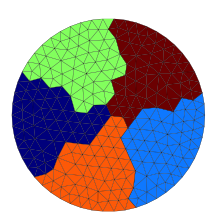
\includegraphics[width=0.3\textwidth]{Figures/Chapters/Parallelisation/parmetisPartition}
 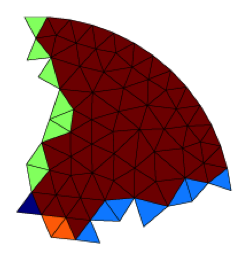
\includegraphics[width=0.2\textwidth]{Figures/Chapters/Parallelisation/parmetisDataPartition}
\caption{Left: Partition of a circle given by parMETIS. Each color represents a different processor on which calculations for that processor should be performed. Right: Data partition of elements for a single processor (red) for circle}
\label{parmetis-figure}
\end{figure}

The nodal values to communicate between processors is be established in the preprocessing state, prior to computation. By parsing the graph and communication each processor recieves a list of elements for computation and the processors to which their nodal values should be sent and a list of interface elements ordered by processors number on which calculations occur. The vector of unknowns $U$, is implemented as a 1-dimensional array. By using the sendtoall functions available through the MPI library the elements numbering can be done in such a way that the MPI buffer recieved is a contiguous section of the vector U. this removes the need for a map of nodal values or copying values between the MPI buffer and the vector $U$.

The solution can be advanced in time following the exact procedure as the serial code, for a single partition of the domain per processor, provided that at each stage of the RK4 method the the nodal solution values should are communicated.

\section{Ordering of Faces}

One caveat to this system is that the addition operation the summation over gauss points to perform the intergration of $A_n^-1$ over the faces must be performed in exactly the same order on both processors. Since at a binary level $$A + B \ne B + A$$ performing the summation in a different order would result in a slightly differing value of on each processor and would destroy the stability of the scheme as illustrated by the example in figure \ref{stability-faces}.

\begin{figure}[htbp!]
 \centering
 \includegraphics[width=0.6\textwidth]{Figures/Chapters/Parallelisation/stabilityFaces}
 \caption{Some kind of figure to illustrate the scheme blowing up for different summation order}
 \label{stability-faces}
\end{figure}

In order to ensure a consistent value between processors the direction of summation of gauss points is always taken with respect to the face with the lowest global index.

% Should I talk about how I do this? How the faces info changes? etc?
% Kahan summation algorithm

\section{Performance And Validation}

% distribution of elements between processors - significance.
The key variable of interest when considering the performance of a parallelised process is the increase in speed obtained when the same problem is attempted on a different number of processors. Since each processor steps in sync the increase in speed will depend primarily on the ratio of time spent on computation for the slowest processor to total time spent communicating the solution. For this reason it is important to optimise not only the time spent on communication but also to ensure that each processor has a similar workload. For this reason allocation of elements to processors according to the time taken to calculate them is important. We also expect a small mesh of a given type element and order of shape functions to have a much less significant improvement in computation that a larger mesh of the same elements. Similarily the same mesh will see a more marked increase in performance for higher order shape functions. Figure \ref{performance2D} illustartes the performance increase attained with increasing number of processors for a 2-dimensional mesh of triangular elements for shape functions of order 2,3 and 5. Figure \ref{performance3D} similarily illustarted the performance increase attained in 3D. We see clearly the advantages of parallelisation for large meshes with higher-order shape functions and larger number of unknowns per element.
% I can also talk about the size of the mesh and the effect the partition has - since this implies less computation
In Figure \ref{uneven-split} we see a system of non-uniform element order. In this case we see that a partition which does not account for this may not perform optimally. Additionally in Figure \ref{timings} we can see that relationship between the difference between partition calculation times and the performance increase for that partition for a given mesh and also the difference between calculation times for different partition of the same mesh.

\begin{figure}[htbp!]
 \centering
 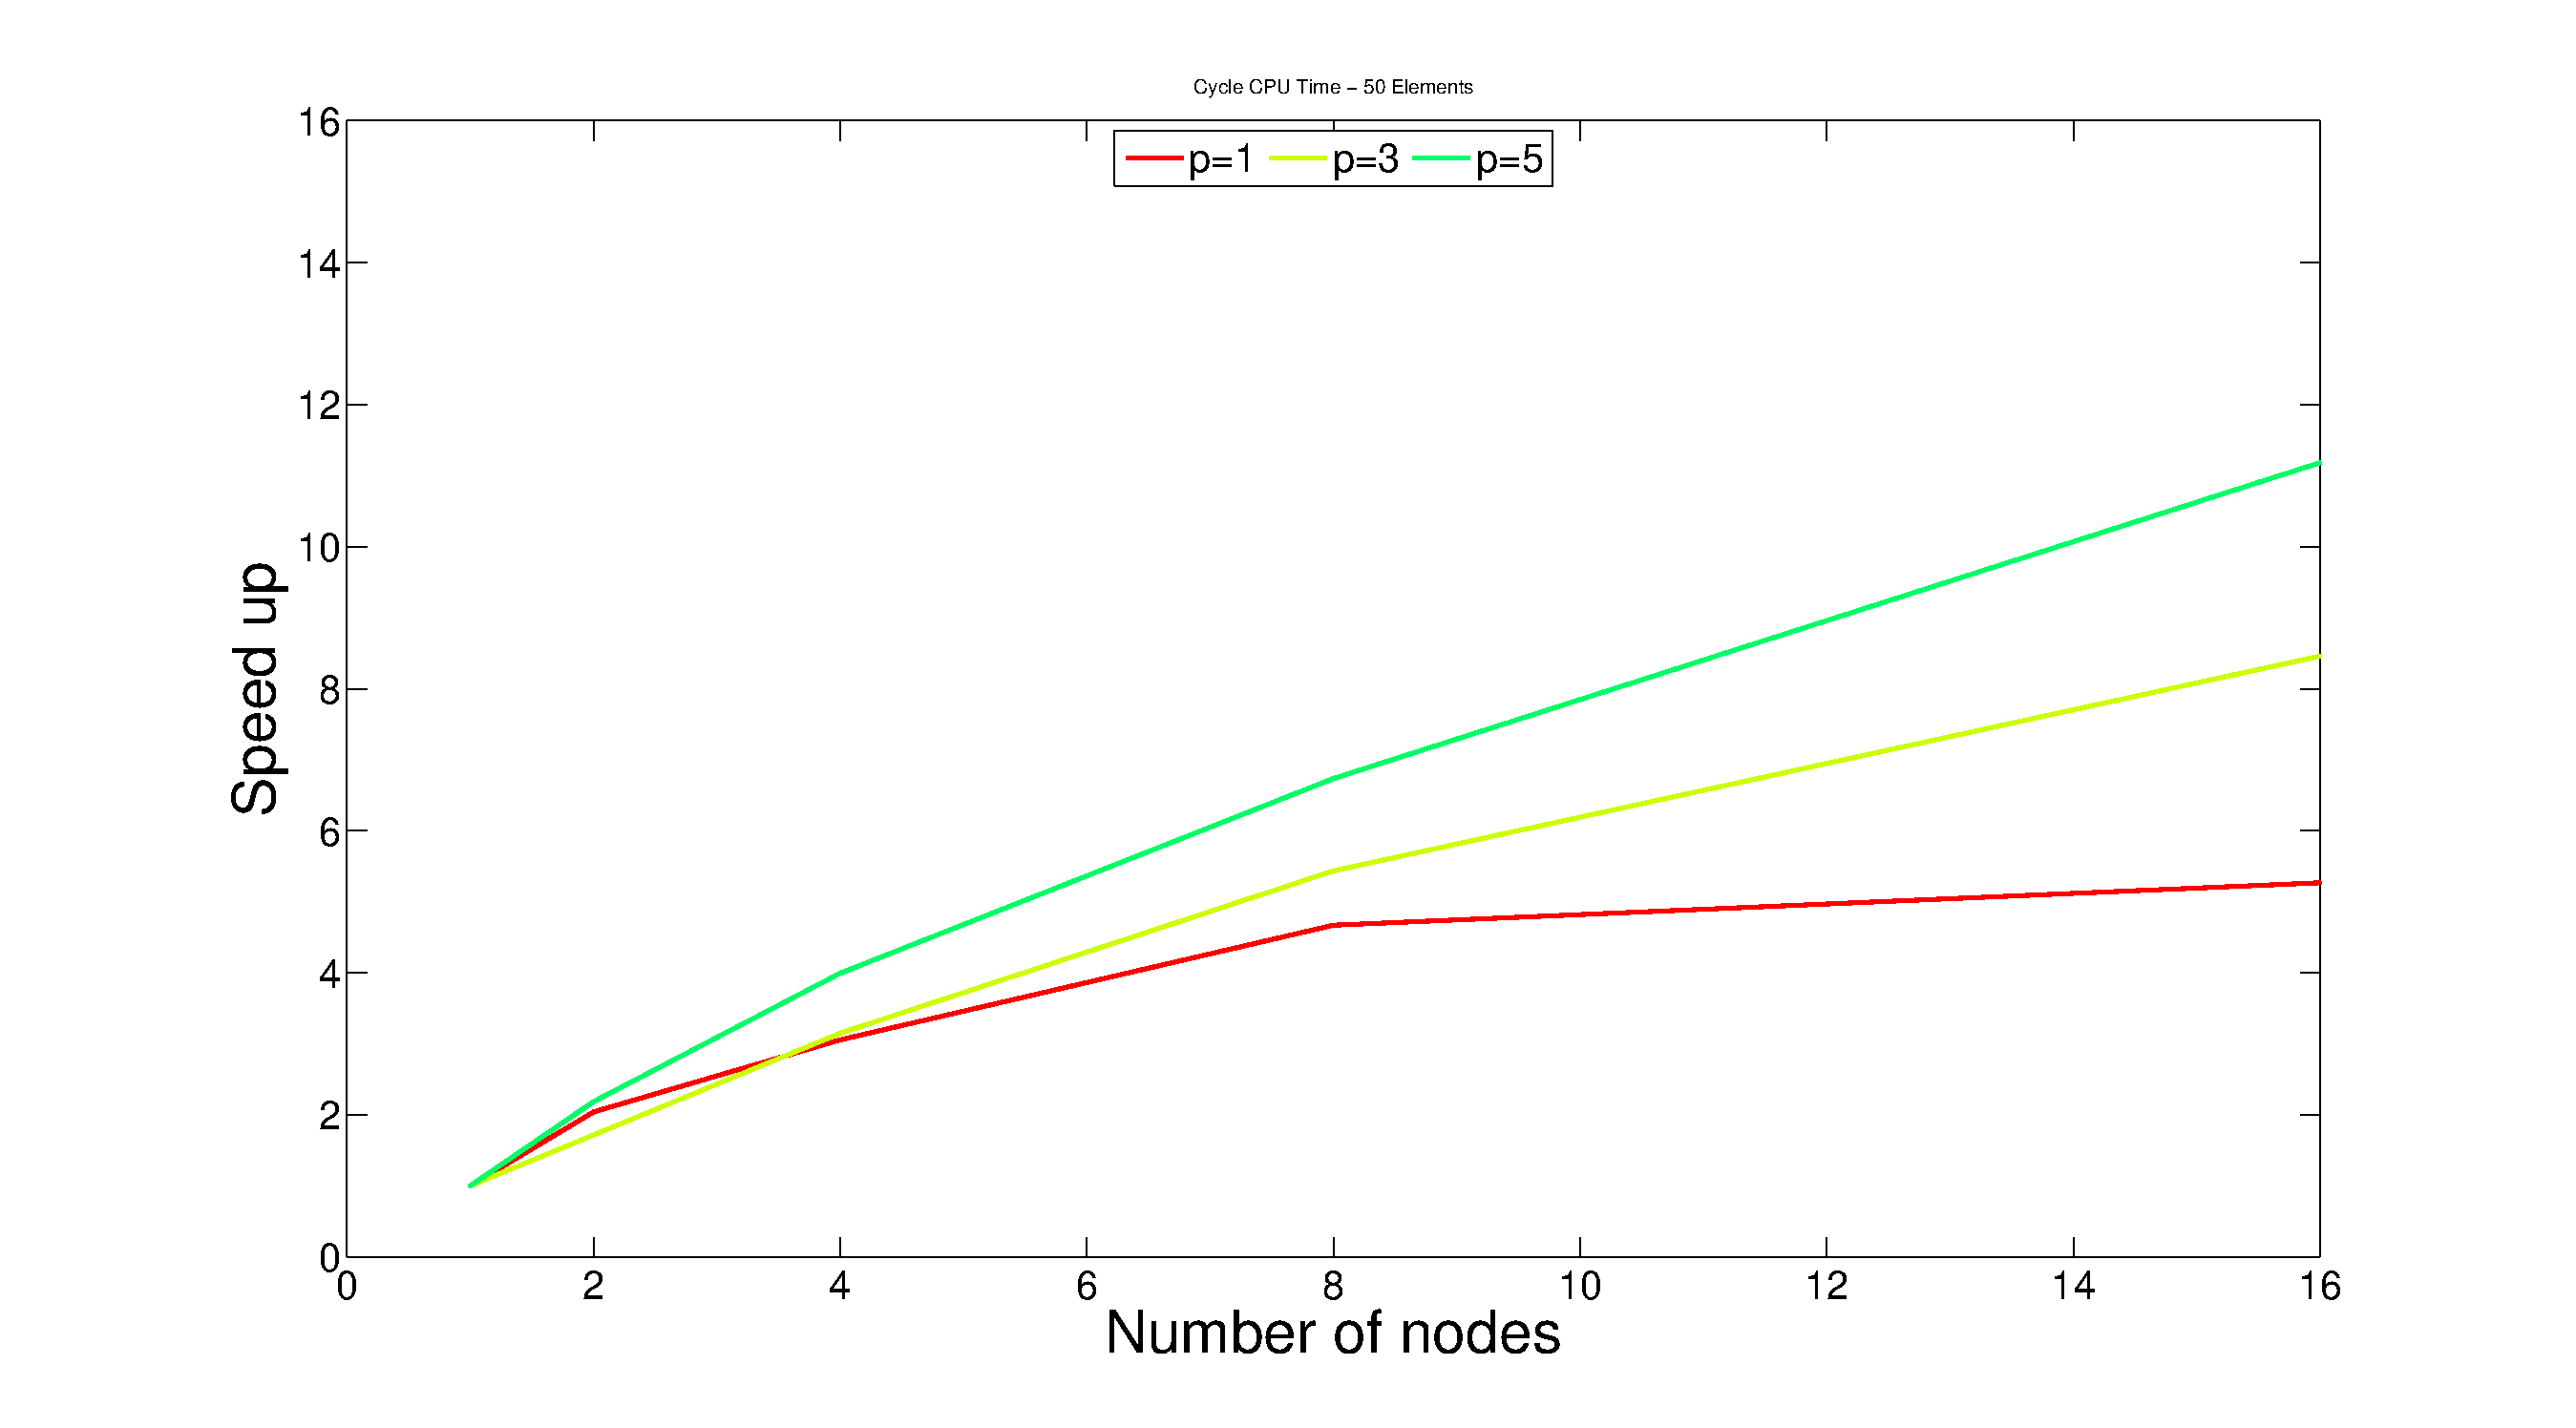
\includegraphics[width=0.45\textwidth]{Figures/Chapters/Parallelisation/speedUp2D/50Elements}
 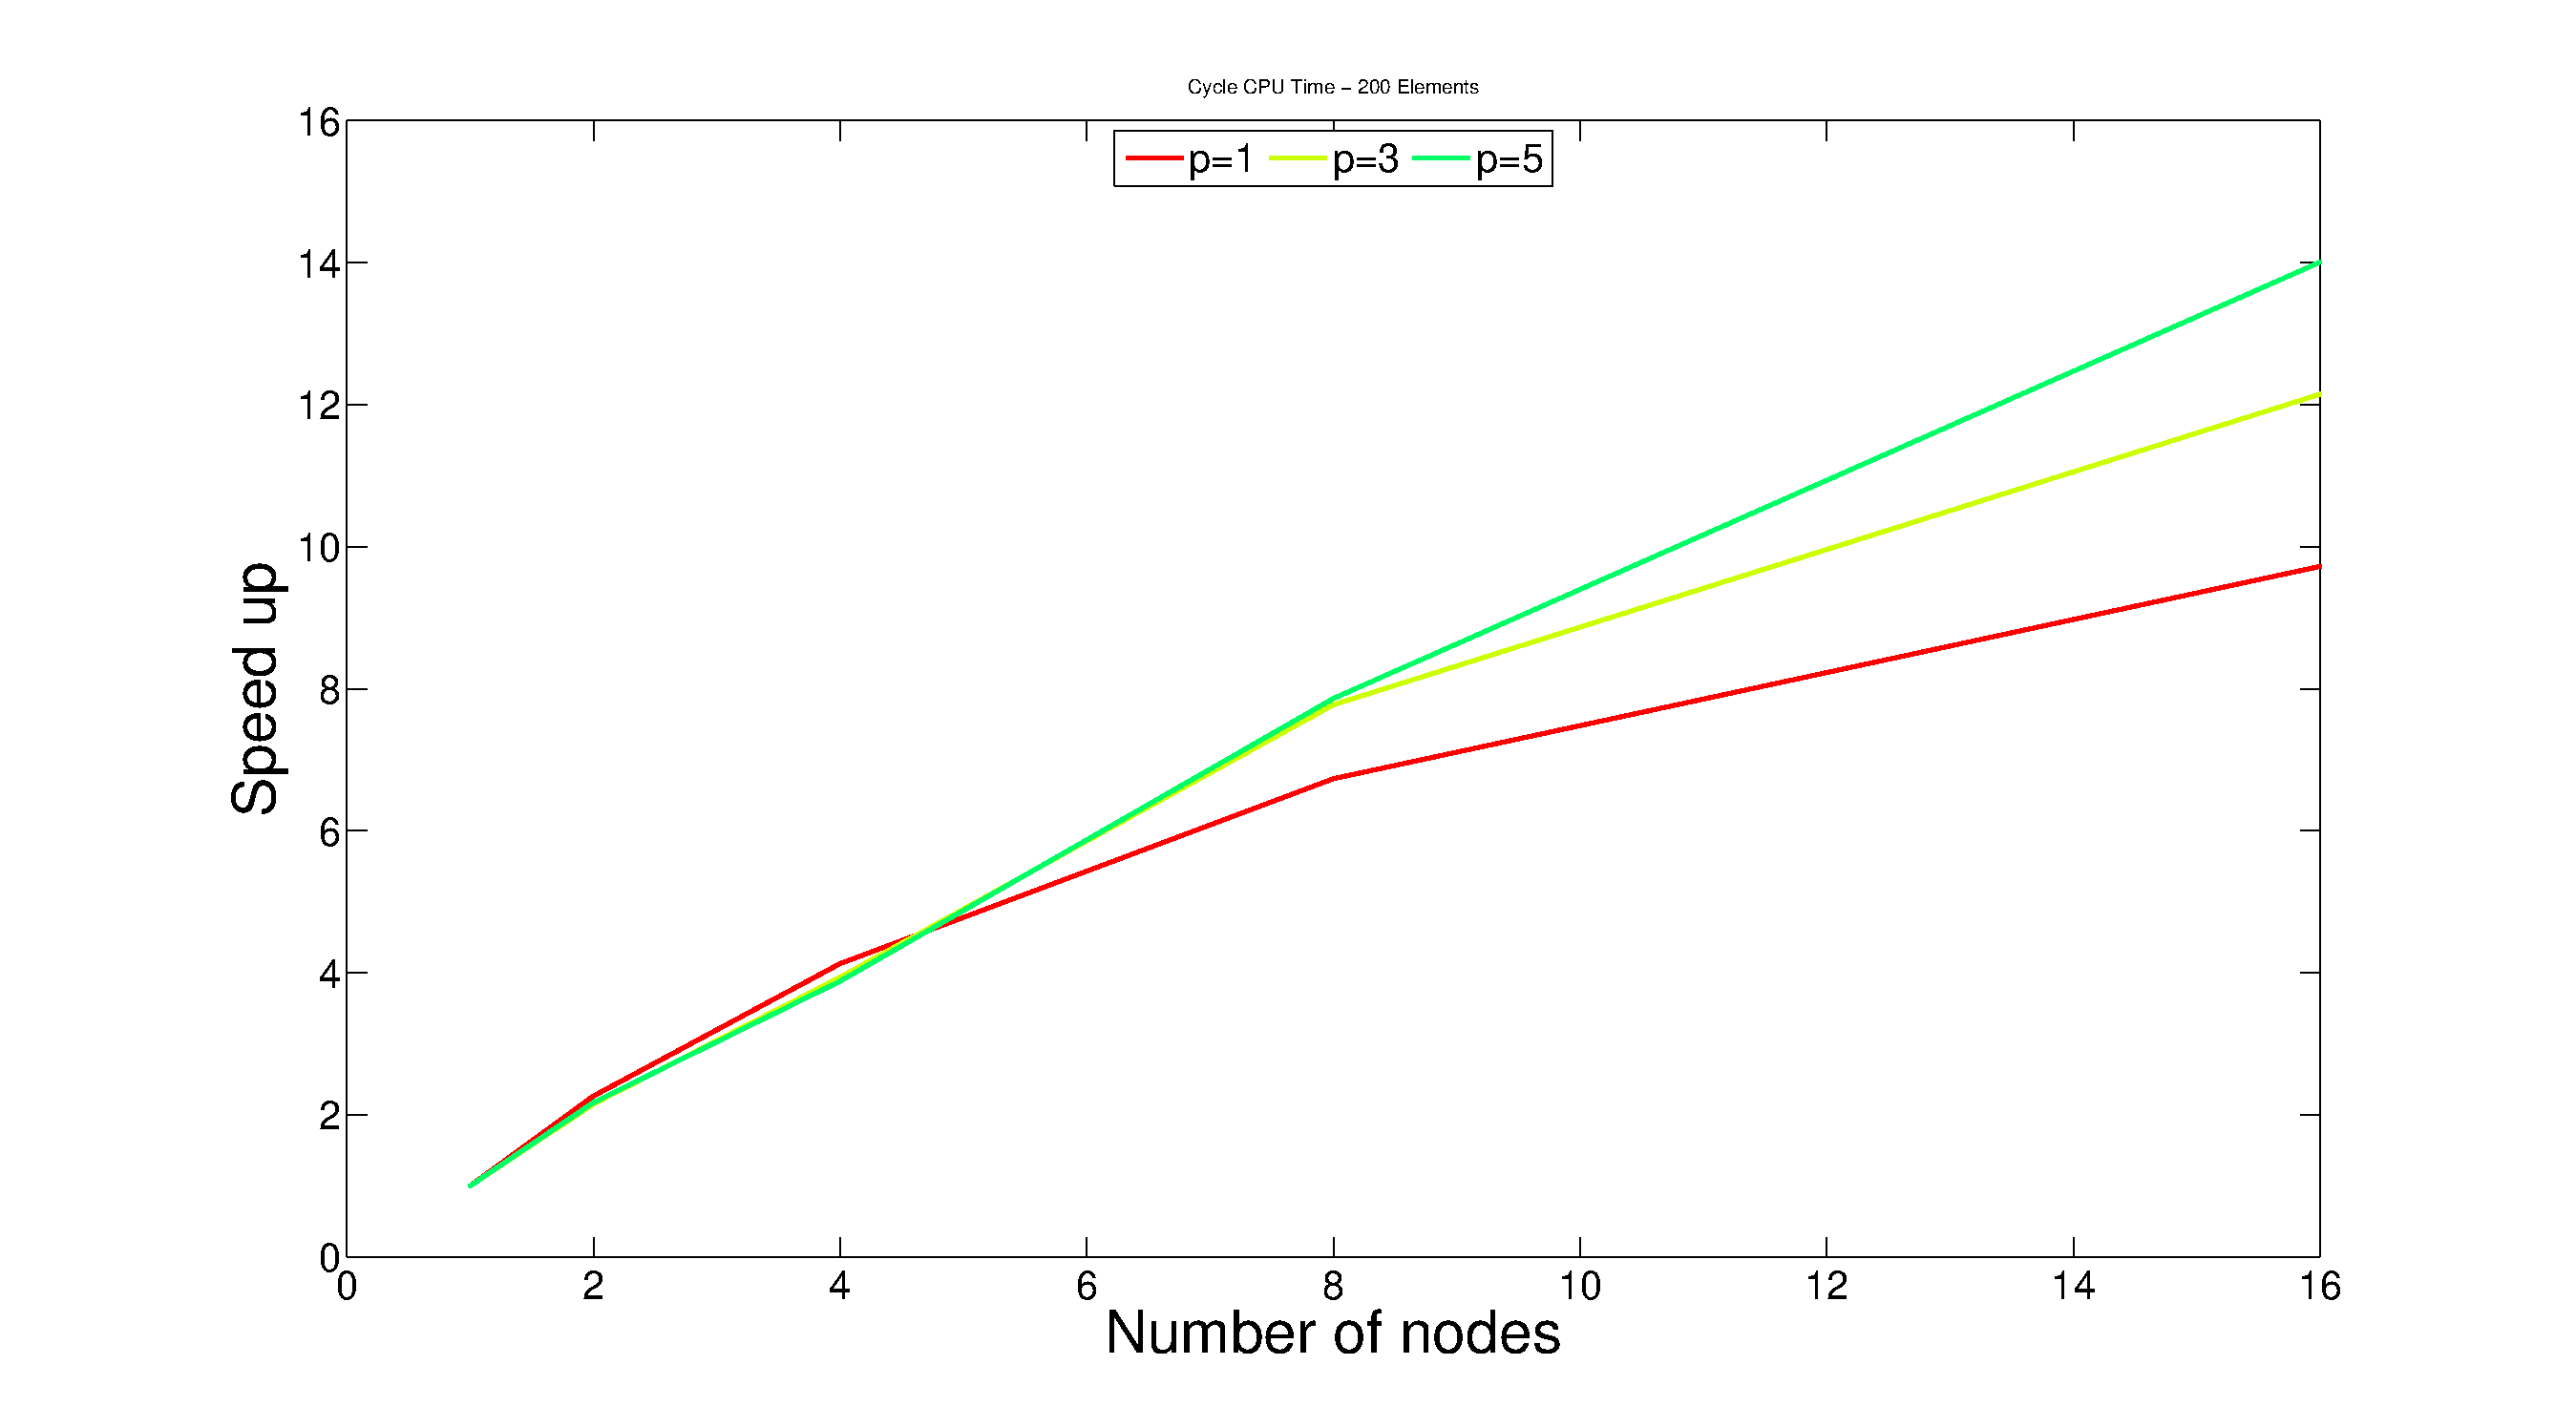
\includegraphics[width=0.45\textwidth]{Figures/Chapters/Parallelisation/speedUp2D/200Elements}
 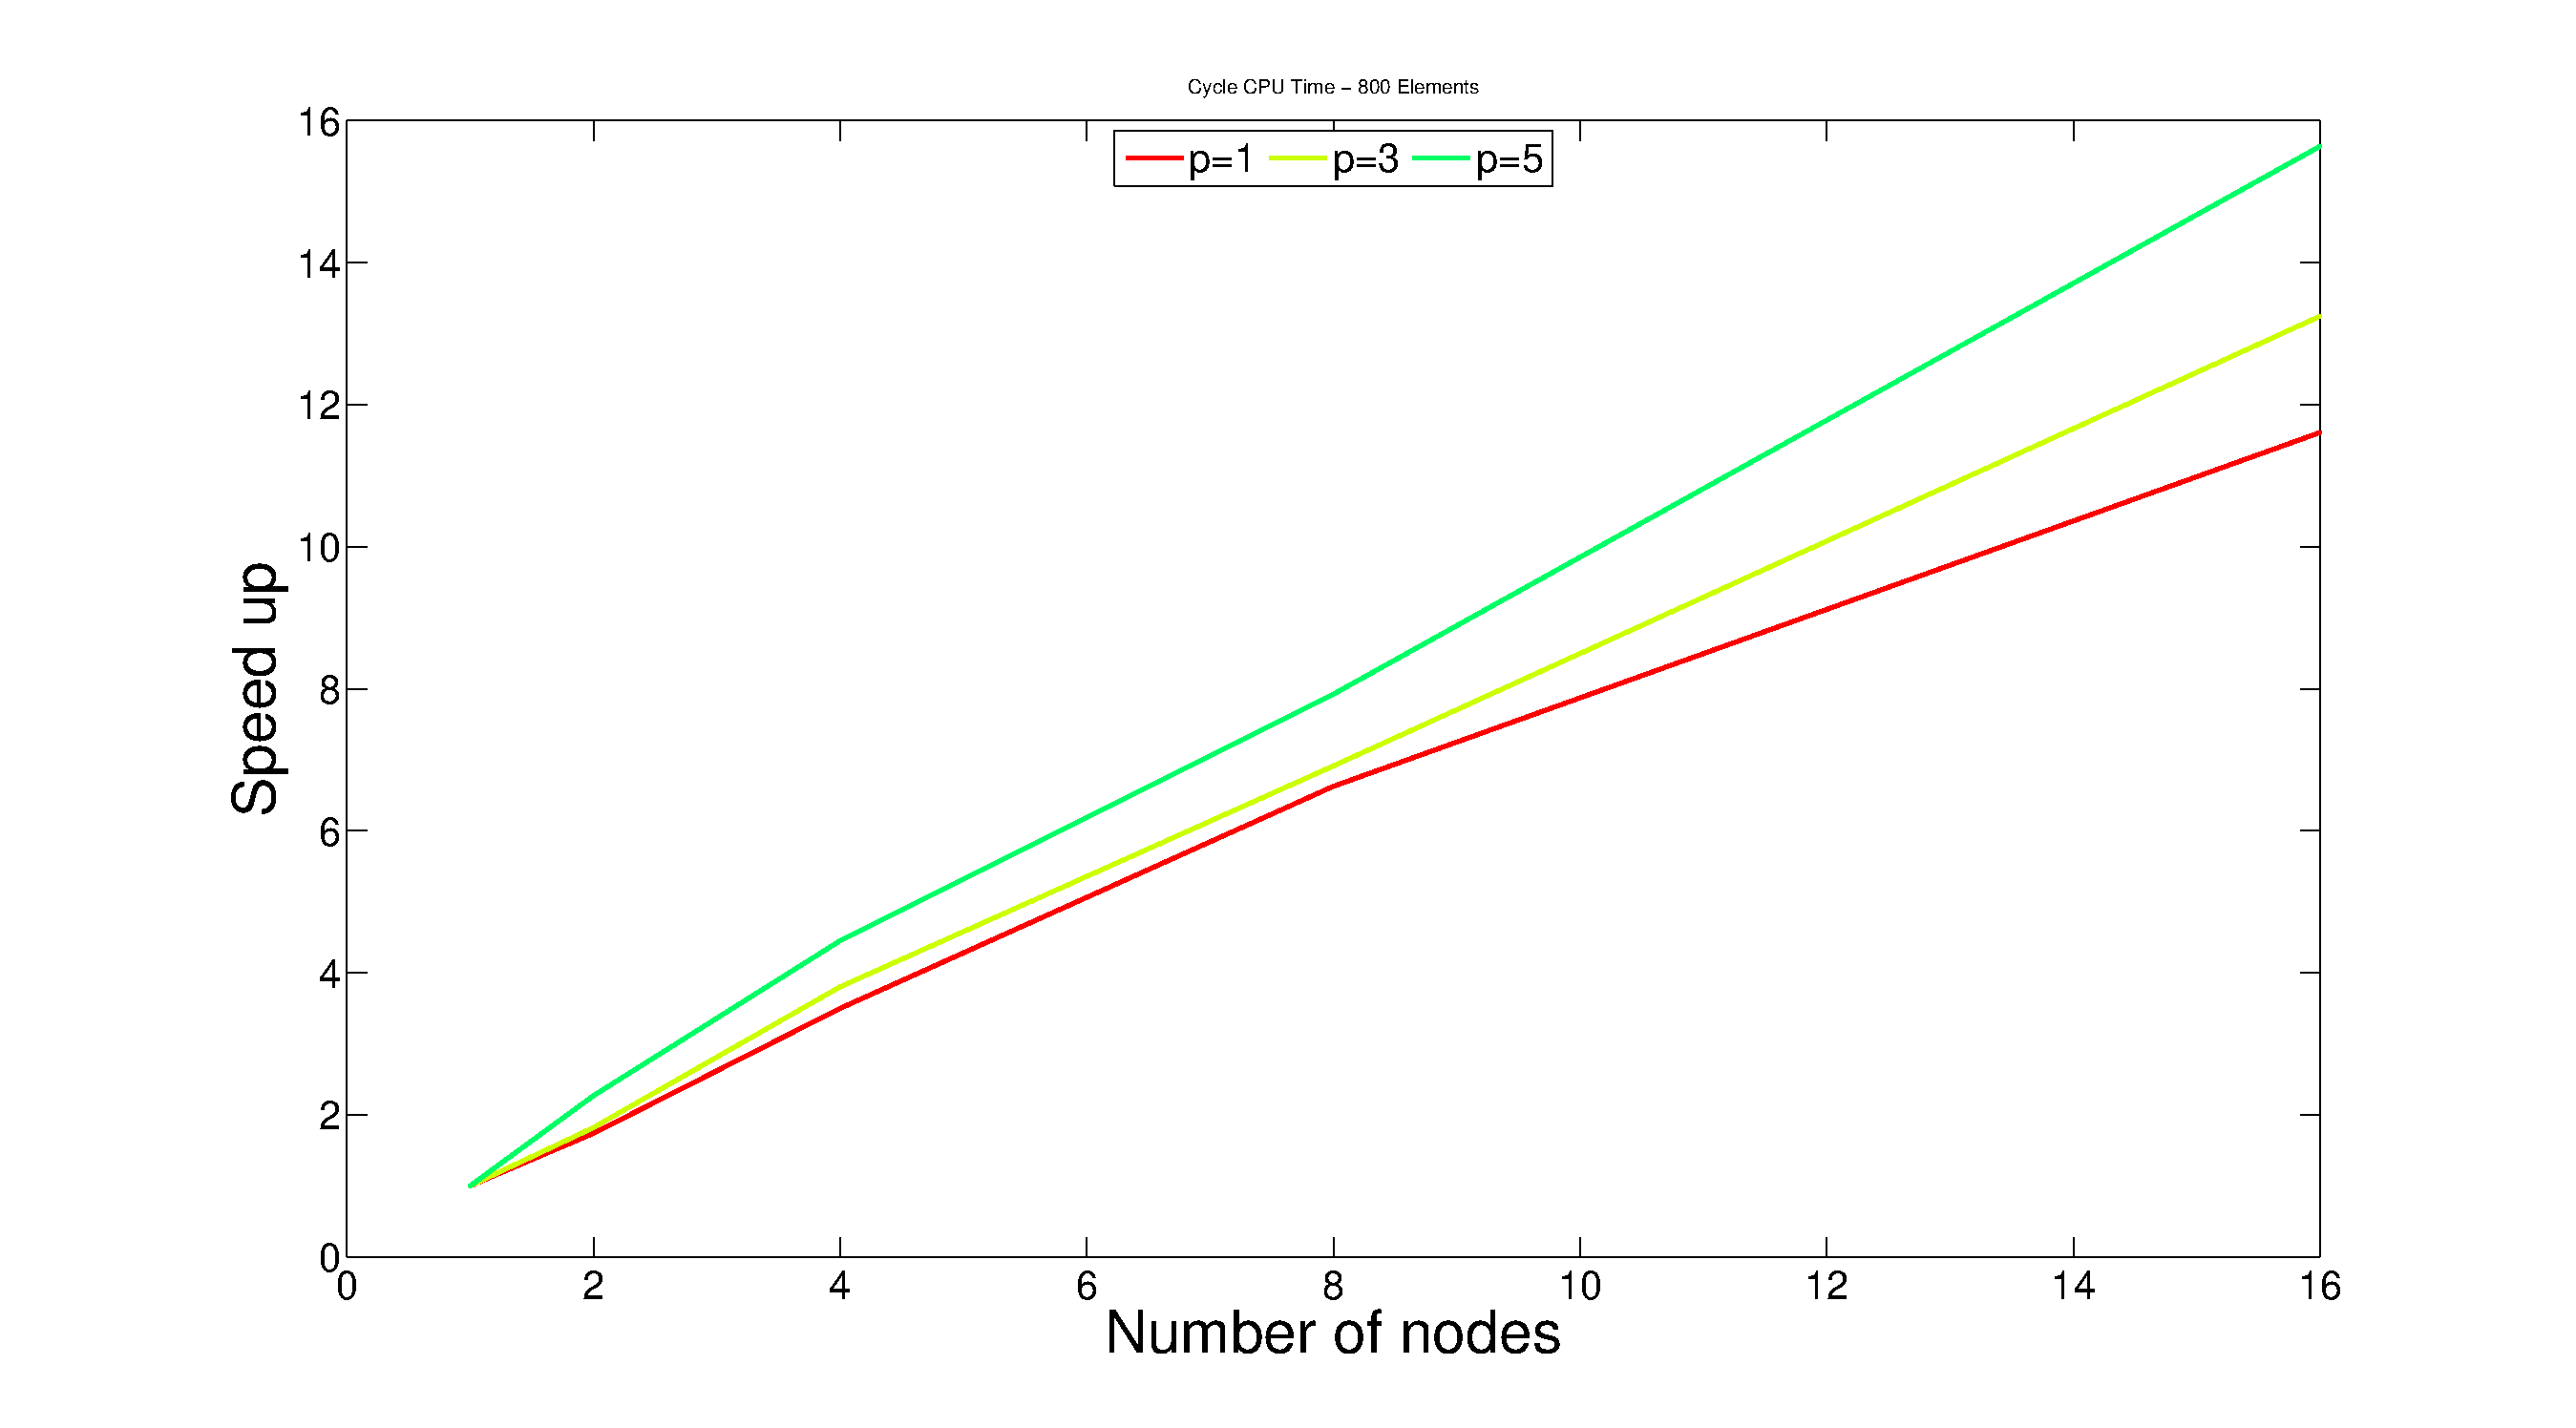
\includegraphics[width=0.45\textwidth]{Figures/Chapters/Parallelisation/speedUp2D/800Elements}
 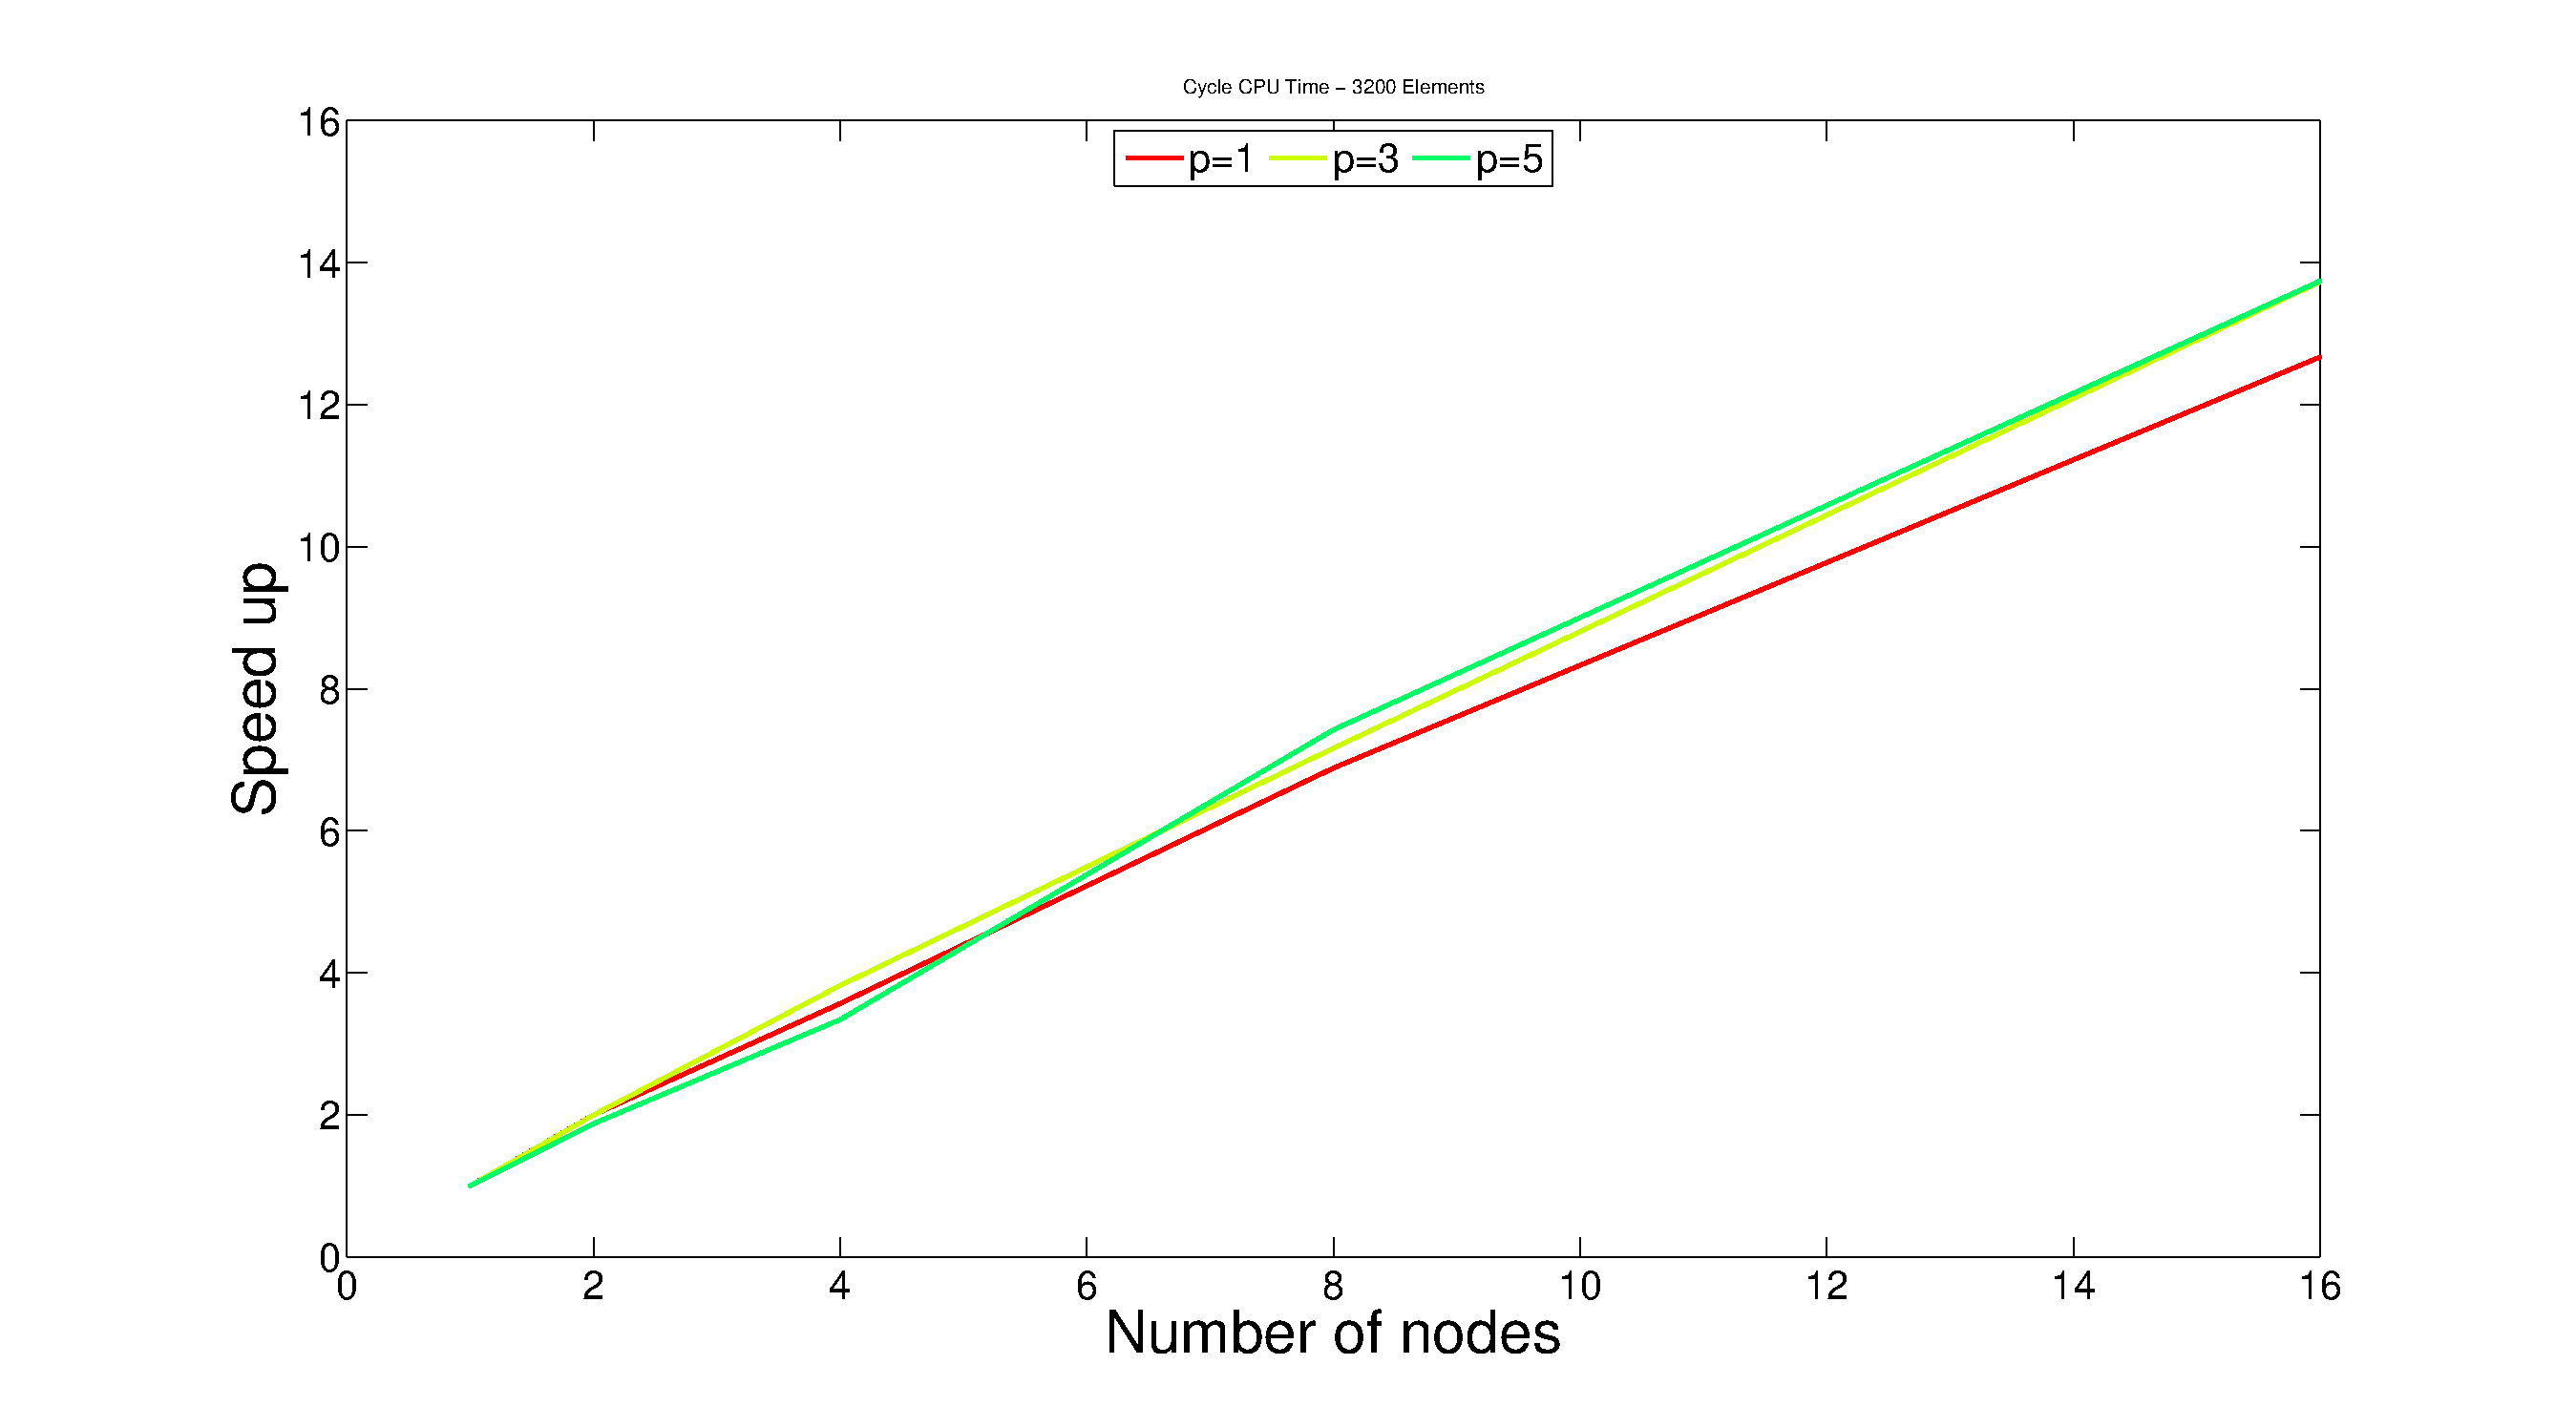
\includegraphics[width=0.45\textwidth]{Figures/Chapters/Parallelisation/speedUp2D/3200Elements}
 \caption{Figure to illustrate the speed up attained for different meshes in 2D}
 \label{stability-faces}
\end{figure}

\begin{figure}[htbp!]
 \centering
 \includegraphics[width=0.45\textwidth]{Figures/Chapters/Parallelisation/speedUp3D/speedUp}
 \caption{Figure to illustrate the speed up attained for different meshes in 3D}
 \label{stability-faces}
\end{figure}

%\chapter{Signal Analysis}
\label{Ch:SignalAnalysis}
\lhead{Chapter 6. \emph{Signal Analysis}} % Write in your own chapter title to set the page header

Resonance is an important phenomena in a number of engineering applications, characterised by quantities such as resonant frequencies, quality factors and mode shapes. The advantage of time domain simulations is that a broadband frequency response can be obtained in a single run. However the the frequency content isn't readily available and needs to be extracted from the obtained time domain evolution of the system. In this chapter we will discuss the fourier decomposition of the time domain solution using parametric and non-parametric methods and the errors associated with this transformation.

\section{Fourier Decomposition}

Fourier transform is a techniques which permits decomposition of any time-domain signal into its frequency domain representation. Based on the Fourier series in which a periodic time domain signal $s(t)$, with a period $T$ such that $s(x)=s(x+nT)$ for $n=1,2,3 ...$ can be written on the interval $(-l,l)$ as

$$
s(t) = a_0 + \sum_{n=1}^{\infty} a_n cos(\frac{n\pi x}{l}) + b_n sin(\frac{n\pi x}{l})
$$

where the fourier coefficients are given by:

$$
a_0 = \frac{1}{2l}\int_{-l}^{l} s(x) dx
$$

$$
a_n = \frac{1}{l}\int_{-l}^{l} s(x) cos(\frac{n \pi x}{l}) dx
$$

$$
b_n = \frac{1}{l}\int_{-l}^{l} s(x) sin(\frac{n \pi x}{l}) dx
$$

If $s(x)$ is only defined on $(-l,l)$ this is equivalent to extending $s(x)$ periodically with a period $2l$. Using eulers equations this can be rewritten as

$$
s(x) = \sum_{n=-\infty}{\infty} c_n e^{\frac{i n \pi x}{l}}
$$

In order to deal with functions on the interval $(\infty,\infty)$ the interval is extended such that the functions is considered periodic with an infinite period. If $s(x)$ is absolutely integrable over the interval $(-\infty,\infty)$ a change of variable $\omega = n \pi / l$ and allowing $l \lim \infty$ results in the summation becoming an integral and $s(x)$ in the interval $(0,\infty)$ can be expressed as

$$
s(x) = \int_{0}^{\infty} \left( A(\omega) cos(\omega x) + B(\omega) sin(\omega x) \right) d\omega
$$

where

$$
A(\omega) = \frac{1}{\pi} \int_{-\infty}^{+\infty} f(u) cos(\omega u) du
$$

and

$$
B(\omega) = \frac{1}{\pi} \int_{-\infty}^{+\infty} f(u) sin(\omega u) du
$$

are known as the fourier coefficients. As above this can be written using the euler relations in complex form as

$$
f(x) = \frac{1}{2 \pi} \int_{-\infty}^{+\infty} \int_{-\infty}^{+\infty} f(u) e^{- i \omega (u - x)} du d\omega
$$

which can be written as

$$
f(x) = \sqrt{\frac{1}{2 \pi}} \int_{-\infty}^{+\infty} \left( \sqrt{\frac{1}{2 \pi}} \int_{-\infty}^{+\infty} f(u) e^{- i \omega u} du \right) e^{i \omega x} d\omega
$$

the expression in brackets is known as the Fourier transform, $F(\omega)$, of the function $f(x)$ and can be written as

$$
\hat{s}(\omega) = \sqrt{\frac{1}{2 \pi}} \int_{-\infty}^{+\infty} f(x) e^{- i \omega x} dx
$$

The Fourier transform of $s(t)$, denoted as $\hat{s}(f)$, is a complex function of frequency whos magnitude and complex argument represent respectively the amplitude and phase offset of the infinite series of sinosoidal functions of which $s(t)$ is composed. The Fourier transform of a continuous signal can be denoted as

$$
\hat{s}(f) = \int_{-\infty}^{+\infty} s(t) e^{-2 \pi i t f} dx
$$
.

If the signal $s(t)$ is known only at a discrete number of times $t_k$ such that $s_k = s(t_k)$, we can rewrite the fourier transform as

$$
\hat{s}_k = \sum_{k=0}^{N-1} s_k e^{-2 \pi i n k / N} dx
$$

The Fourier transform in this form is known as the discrete Fourier transform (DFT).

A correctly scaled fourier transform of a time domain signal is known as the power spectrum of the signal.

The continuous fourier transform requires that integration is preformed between $\-infty$ and $\infty$, or over an integer multiple of the periodicity of the signal, $T$. For most sampled signal with multiple frequency components it is not possible in general to measure signals which would be repeated periodically in $T$. That is signals where $s(T) = s(0)$. Such signals extended to infinity would exhibit discontinuities. These discontinuities give rise to a phenomena known as spectral leakage[], in order to capture these discontinuities, which intoduces noise into the system. This is clearly not desirable, and can be reduced by using a window function, such as the Blackman window. The signal is multiplied by and envelope which ensures the discontinuity is eliminated.

A system exhibits resonance if frequency components at the resonant frequencies of the system oscillate with larger amplitudes than away from these resonant frequencies. In this case peaks in power spectrum will be seen at the corresponding resonant frequencies. Resonant frequency values can be recovered by peak fitting. [ mention Lorentz fitting here? compare to spline fitting? ]

*** Fast Fourier Transform ***

The widely used Fast Fourier transform [***] algorith which reduces the computational of the DFT from an $\bigO(n^2)$ operation to an $\bigO(n log n)$ operation.

A discrete fourier transform of a time domain signal leads to a frequency domain spectrum, where an amplitude is associated with evenly spaced, discrete points in a frequency interval. This frequency domain representation of the signal is exact provided that the number of point...***

This frequency amplitude is a complex number denoting the coefficient a given frequency in the discrete fourier series expansion.  This can be convieniently plotted in an amplitude against frequency plot known as a power spectrum, where the peaks of the spectrum corrispond to the resonant frequencies of the system.

The frequency resolution of the spectrum, that is the spacing of the discrete points in frequency space, is given by

$$
\Delta f = \frac{1}{T}
$$

where $T$ is the final time of the simulation. Care should be taken to ensure that the final time of the simulation is sufficiently long to account for the desired simulation error.

% *** I can show this by showing in the results section how closely this matches the actual error found


The maximum frequency, $f_{max}$, which can be resolved by a fourier transform is given by the Niquist-Shannon theorem which states
$$
f_{max} \leq \frac{1}{2 \Delta t_s}
$$

where $\Delta t_s$ is the time between sampling points of the signal, the sampling interval. A time domain signal in which the highest frequency component has a frequency less that $f_{max}$ is represented fully by the frequency domain spectrum. For time domain signals containing components of higher frequency that $f_{max}$ *** aliasing ***.
% what happens here...!?
Clearly the simulation time step, $\Delta t$, gives an upper limit on the sampling interval - therefore care should be taken to choose the $\Delta t$ of the simulation to be sufficiently small to allow the desired $f_{max}$ and also to allow for a sufficiently small error in the time domain signal. Which of these criteria is limiting factor will in general depend on the frequencies of interests.

\section{Resonant Frequencies}
\section{Mode Shapes}

The fourier transform can be thought of as a factorisation of the signal into a temporal and spatial part. For a single point the spatial part will simply be a complex amplitude. However when the entire domain is considered each point has an associated complex amplitude for each frequency, which forms a spatial envelope which when multipled by the temporal part defines the oscillations associated with that frequency. When the frequency considered is a resonant frequency, then the envelope is known as the mode shape associated with that frequency.

\section{Quality Factors}

The quality factor is a widely used in engineering to describe the damping of an oscillating system. The qaulity factor, $Q$, indicates the rate at which energy is dissipated in the system. In applications where resonance is required, engineering a system with a high-Q is usually desirable. In a high-Q system resonant frequency oscillations will have a longer lifetime and less energy need be provided to the system to maintain an oscillation. The Q-factor at a resonant frequency, $f_{res}$ commonly written as the ratio

$$
Q = f_{res}/\B_{FWHM}
$$

where $B_{FWHM}$ is the bandwith of the resonant oscillation at half of its amplitude, commonly known as the full-width-half-maximum (FWHM) value. An equivalent definition can be given in terms of the ratio of energy stored in the oscillator at resonant frequency to the rate of energy loss per cycle

In a resonant optical cavity the quality factor, $Q$, for a given resonant frequency, $f_{res}$, is given by

$$
Q = 2 \pi f_{res} \frac{\Epsilon}{P}
$$

where $\Epsilon$ is the energy stored in the system and $P$, the dissipated power, is given by $-\frac{d \Epsilon}{dt}$.

In resonant system with a high quality factor, resonant frequency oscillations with have a long lifetime. Whilst oscillations away from the resonant frequency will die out quickly. Conversely in a system with a lower Q-factor the resonant oscillations will die out quickly and the resonant peak will have a larger bandwidth. Figure \ref{fig:signal-analysis-low-vs-high-q-spectrum} shows the resonant peaks of a circular PEC cavity, with a high quality factor, and the same signal with dissipation introduced, that is a low quality factor.

\begin{figure}
\begin{center}
    \includegraphics[scale=]{Figures/SignalAnalysis/lowVsHighQualitySpectrum}
\end{center}
\caption{}
\label{fig:signal-analysis-low-vs-high-q-spectrum}
\end{figure}

For a dispersive system this will manifest itself in a wider spectrum line width [], and consequentially a larger error in the quality factor. Note that dispersion could be either physical or could be a non-physical dispersion introduced by a numerical method.

A system with PEC boundaries and no material loss with no numerical errors is expected to have a zero linewidth and infinite quality factor.

%WWWIIK

% *** maybe mention Q-switching - how does Q-switching work? Am I going to research it?

\section{Envelopes}
Since the signals being considered are of finite length, the periodic repetition of a finite signal results in a discontinuity, unless the final and initial values of the signal match exactly. This gives rise to a phenomena called spectral leakage, where non-physical non-zero spectral amplitudes are observed. For example consider a signal consisting of a single frequency

$$
f(x) = sin(i2 \pi f_{res} x)
$$
.

Then taking a discrete Fourier transform of the signal over a finite interval leads to spectral leakage as illustrated in figure \ref{fig:signal-analysis-speactral-leakage-sine-wave}. Note that for longer periods, less leackage occurs. Also note that figure {***} has significant lower leakage than figure {***} with a similar signal length. This is due to the signal in figure {***} having an integer multiple of cycles, resulting in a signal which can be repeated periodically exactly.

\begin{figure}
\begin{center}
    \includegraphics[scale=]{Figures/SignalAnalysis/spectralLeakageSineWave}
\end{center}
\caption{Fourier transform of a number of sine waves with different intervals}
\label{fig:signal-analysis-speactral-leakage-sine-wave}
\end{figure}


These non-physical frequencies due to a finite interval can be reduced by multiplying the signal by a suitable window function prior to performing the DFT. This ensures that the initial and final values are zero.
% This will introduce an additional periodicity the length of the signal...
There are a number of choices of window, which should be selected according to the expected frequency content of the time domain signal.  We use the popular Blackman envelope [***] prior to Fourier transforms in all examples in this work, unless specified otherwise. The Blackman envelope is given by
% REF: Blackman, R. B. and Tukey, J. W. "Particular Pairs of Windows." In The Measurement of Power Spectra, From the Point of View of Communications Engineering. New York: Dover, pp. 98-99, 1959.
$$
A(x) = \frac{21}{50} \frac{1}{2} cos ( \frac{\pi x}{a} ) + \frac{2}{25} cos ( \frac{2 \pi x }{a} ) 
$$

A short sample signal with a filter applied is shown for illustration in figure \ref{fig:signal-analysis-blackman-envelope}, alongside examples of spectra obtained from the same signal with and without the filter to illustrate the spectral leackage effect.

\begin{figure}
\begin{center}
    \includegraphics[scale=]{Figures/SignalAnalysis/blackmanEnvelope}
\end{center}
\caption{Blackman envelope applied to a superposition of two sin waves + the spectrum of the superpositionof two sine waves of frequencies *** and *** with and without a blackman filter applied }
\label{fig:signal-analysis-blackman-envelope}
\end{figure}

Figure \ref{fig:signal-analysis-comparison-of-envelopes} show the spectrum of the same time domain signal alongside the spectrum shown after applying a number of popularly used filters and the shape of these filters.

\begin{figure}
\begin{center}
    \includegraphics[scale=]{Figures/SignalAnalysis/comparisonOfEnvelopes}
\end{center}
\caption{}
\label{fig:signal-analysis-comparison-of-envelopes}
\end{figure}

\section{Need to explain the whole end to end process}

%% : possible comparison of different
\section{Zero frequency}
If the frequency does not osciallate about zero, this will manifest itself in the spectrum as a peak centered on zero. This will occur of example when in a non-dissipative case the signal is sampled near a point where the cavity was excited. It is therefore advisable when possible to pick a point to sample a signal which is far from the source point.

\section{Fitting Parameters}

Lorenzian fitting assume a shape of the wave as

$$
e^{.../\tau}
$$

transformed into frequency space. We can use a Lorenzian fitting with a least squares approach to obtain a good fit for a peak - provided that the peak is isolated. However if the peak is near other peaks this can become a problem.

%some solution would be required to fit the lorenzian to the peak.

\section{Parametric Methods}

Parametric methods such as the filter diagonalisation method (FDM) use an assumption of the shape of the signal to find the resonant frequencies by solving an eigenvalue problem. This method can be used to significantly reduce the error in the number time steps required to reach a solution. In numerical experiements a increase of an order of mangnitude was observed for FDM over FFT.

However parametric methods are sensitive to dispersion which can degrade the signal amplitude for signals which are of a considerable length, and therefore while a better result can be obtained for a short run, for longer runs required to obtain a high accuracy the method is unsuitable.

\begin{itemize}
  \item present the basis of the FFT method
  \item dependence of resolution/cut-off
	\item window functions / blackman envelope
	\item filter diagonalisation method
	\item Modal Shapes - how to obtain modes from resonant frequencies
  \item comparison of the FFT + FDM
  \item Summary of complete methods to recover resonant frequencies for a given problem
\end{itemize}

% % Chapter 1

\chapter{Analytical Investigations} % Write in your own chapter title
\label{Chapter 4}
\lhead{Chapter 4. \emph{Analytical Investigations}} % Write in your own chapter title to set the page header

\section{Mesh Refinement Study for Analytical Solutions}
A study of FFT and FDM methods using an analytical wave shape were performed to try and determine how the method is affected by signal length and mesh interpolation. The waves studied are of the form:
$$
E(x,t) = \sum_i sin(kx - \omega_i t)
$$
Take two spatial points $x_1$ and $x_2$, which are a distance $\Delta x$ appart. Choose a point $x_0$ which is half way between these two points, and represent the value at that point as a linear interpolation of the values at $x_1$ and $x_2$.
$$
E(x_0,t) = \frac{1}{2} \left[ E(x_1,t) + E(x_2,t) \right]
$$

The studies in this section were performed with a single and multiple frequencies ($\omega_i$) however no major differences were found and the results presented here are for f=100 ($\omega = 2 \pi f$);

The idea is then to cary $\Delta_x$ and investigate the effect of the mesh on the signal achieved. This is illustrated in figure \ref{MonitorPointMeshRefinement_waves_in_space} which shows the spatial, analytical waves in space at time $t=0$ and a line showing the linear approximation being used to find the value at $x_0$ for 9 different values of $\Delta x$. These 9 different values of $\Delta x$ will be used throughout the study. Clearly depending on the size of $\Delta x$ there will be a phase difference in the signals between the sampled points at $x_0$, $x_1$ and $x_2$. A very small $\Delta x$ will give a signal shape very close to signal both at $x_1$ and $x_2$. The larger values of $\Delta x$ however give a linear interpolation with a larger phase difference and the phase difference between the wave at point $x_0$ and $x_1$ in space determines the amplitude. Figure \ref{MonitorPointMeshRefinement_waves_in_time} shows analytical values for signals at $x_0$, $x_1$ and $x_2$ while Figure \ref{MonitorPointMeshRefinement_waves_approx_in_time} shows the analytical values at $x_0$ (the same as those in Figure \ref{MonitorPointMeshRefinement_waves_in_time}) compared to the linear interpolations obtained at $x_0$. Figure \ref{MonitorPointMeshRefinement_waves_approx_in_time} shows that the linear interpolations for the selected $\Delta x$ values vary visibly from the analytical values of the waves sampled at the same point. Values of $\Delta x$ in which the points selected are in phase show an interpolated wave which is in phase. Whilst points out of phase show waves with a very different phase and amplitude.

\begin{figure}
    \subfigure[Waves for t=0 in space showing the linear approximation being used for each $\Delta x$.]{
        \includegraphics[width=0.48\textwidth]{Figures/1D_Analytical_Study/MonitorPointMeshRefinement/waves_in_space.png}
        \label{MonitorPointMeshRefinement_waves_in_space}
    }
    \subfigure[This plot shows the exact (analytical) values of the waves sampled in time at points $x_0$ (green), $x_1$ (blue) and $x_2$ (red).] {
        \label{MonitorPointMeshRefinement_waves_in_time}
        \includegraphics[width=0.48\textwidth]{Figures/1D_Analytical_Study/MonitorPointMeshRefinement/waves_in_time.png}
    }
    
    \subfigure[Values obtained at $x_0$ by linear interpolation (blue) and the corrisponding analytical values at $x_0$ (green) for different $\Delta x$.]{
        \label{MonitorPointMeshRefinement_waves_approx_in_time}
        \includegraphics[width=0.48\textwidth]{Figures/1D_Analytical_Study/MonitorPointMeshRefinement/waves_approx_in_time.png}
    }
    \caption{Analytical and interpolated waves in space and time}
    
    \label{MonitorPointMeshRefinement}
\end{figure}

\begin{figure}
    \subfigure[FFT spectrum from waves sampled for 1000 cycles. Waves with different mesh sizes appear to be have different spectral amplitudes.]{
        \includegraphics[width=0.66\textwidth]{Figures/1D_Analytical_Study/MonitorPointMeshRefinement/waves_in_time_fft.png}
    }
    
    \subfigure[Peak frequency error in the two frequency components from the analytical frequency]{
        \includegraphics[width=0.66\textwidth]{Figures/1D_Analytical_Study/MonitorPointMeshRefinement/PeakFreqError.png}
    }
    \caption{Frequencies Calculated from FFT of signal in time obtained from interpolation at various $\Delta x$s}
    \label{MonitorPointMeshRefinement_FFT}
\end{figure}

\section{Timestep Refinement Study for Analytical Solutions}

A the same analytical wave shapes are used
$$
E(x,t) = \sum_f sin(kx - \omega_f t)
$$
where
$$
\omega_f = [ 100, 120, 1000, 500, 300 ]
$$

\begin{figure}
\includegraphics[width=\textwidth]{Figures/1D_Analytical_Study/MonitorPointDtRefinement/waves_in_time.png}
\caption{Original signal in time with red line showing points selected for approximation}
\end{figure}

\begin{figure}
\includegraphics[width=\textwidth]{Figures/1D_Analytical_Study/MonitorPointDtRefinement/waves_in_time_fft.png}
\caption{Spectrum FFT - cut off point visible}
\end{figure}

\begin{figure}
\includegraphics[width=\textwidth]{Figures/1D_Analytical_Study/MonitorPointDtRefinement/PeakFreqError.png}
\caption{Frequencies plotted up to cutoff point}
\end{figure}

\begin{figure}
\includegraphics[width=\textwidth]{Figures/1D_Analytical_Study/MonitorPointDtRefinement_byDoubling/PeakFreqError.png}
\caption{Frequencies plotted against cutoff (more points)}
\end{figure}
% % Chapter 1

\chapter{2D Plate} % Write in your own chapter title
%\label{Chapter3}
\lhead{Chapter 3. \emph{Results}} % Write in your own chapter title to set the page header

\section{fake wave}

\begin{figure}
\includegraphics[width=\textwidth]{Figures/2D_FEM_Propagation_MPI/errorSignal_0_5x100_domain}
\caption{Error for shorter domain - 0.5x100 - with envelope IC and no evelope - PEC on all sides except LHS with dirichlet boundary. BC=100 and 106(with envelope)}
\end{figure}

\section{Signal and error in Signal - 0.5x100 domain}

\begin{figure}
\includegraphics[width=\textwidth]{Figures/2D_FEM_Propagation_MPI/errorSignal_0_5x100_domain}
\caption{Error for shorter domain - 0.5x100 - with envelope IC and no evelope - PEC on all sides except LHS with dirichlet boundary. BC=100 and 106(with envelope)}
\end{figure}

\begin{figure}
\includegraphics[width=\textwidth]{Figures/2D_FEM_Propagation_MPI/FDM_forAnalyticalWave}
\caption{Error in the frequency calculated by FDM for an analytical wave of the same shape as the wave being studied sampled at a point [0.25,0.25]}
\end{figure}

\begin{figure}
\includegraphics[width=\textwidth]{Figures/2D_FEM_Propagation_MPI/PeriodConvFreq}
\caption{Convergence of error in frequency with period. Measure at point [1.0000,0.2500] in 10x0.5 domain. Signals with no initial condition were sampled from t=4}
\end{figure}

\begin{figure}
\includegraphics[width=\textwidth]{Figures/2D_FEM_Propagation_MPI/signalValueWithoutInitialCondition}
\includegraphics[width=\textwidth]{Figures/2D_FEM_Propagation_MPI/signalAnalyticalVsCalculatedValue}
\caption{Top: Wave solution sampled at 3 points in the domain with no initial condition (shows propagation speed and shape of solution) Bottom: 1280x2 mesh with IC=100 and dirichlet boundary on LHS, PEC top and bottom and ABC on the RHS. Measured at point [0.25,0.25] }
\end{figure}

\begin{figure}
  \begin{centering}
\includegraphics[width=0.7\textwidth]{Figures/2D_FEM_Propagation_MPI/errorInSignalWithTimeStep}
\caption{Error in signal propagation with time for the initial period T=0->50 at point [0.25,0.25]. Error remains fixed after convergence.}
\end{centering}
\end{figure}

\section{Signal and error in Signal - 0.5x300 domain}

Problem: wave propagation, BC=100 in a long cavity length 320.

\begin{figure}
  \begin{centering}
\includegraphics[width=0.7\textwidth]{Figures/2D_FEM_Propagation_MPI/convWithPeriod_variableDT_skipStep1}
\includegraphics[width=0.7\textwidth]{Figures/2D_FEM_Propagation_MPI/convWithPeriod_variableDT_skipStep10}
\includegraphics[width=0.7\textwidth]{Figures/2D_FEM_Propagation_MPI/convWithPeriod_variableDT_skipStep50}
\caption{Error in the frequency calculated by FDM for a signal sampled at a point [0.25,0.25] and for varying periods. Three plots show (top to bottom) signal sampled every 1,10 and 50 timesteps. timesteps are
0.0164,0.0059 and 0.0021 (respectively for refinements 2->4 elements across).
}
\end{centering}
\end{figure}

\begin{figure}
\includegraphics[width=\textwidth]{Figures/2D_FEM_Propagation_MPI/errorInFrequncyWithDt}
\caption{Error in frequency with changing sampling rate after simulation (for a fixed simulation timestep) using a fixed length period (5000)}
\end{figure}

\begin{figure}
    \begin{centering}
\includegraphics[width=0.5\textwidth]{Figures/2D_FEM_Propagation_MPI/maxErrorPerCycle_zoomIn_1280x2}
\includegraphics[width=0.5\textwidth]{Figures/2D_FEM_Propagation_MPI/maxErrorPerCycle_zoomIn_2560x4}
\includegraphics[width=0.5\textwidth]{Figures/2D_FEM_Propagation_MPI/maxErrorPerCycle_zoomIn_8x5120}
\caption{Maximum error per cycle for a 2560x2, 2560x4 and 8x5120 element mesh respectively of a 0.5x320 domain.}
\end{centering}
\end{figure}

\begin{figure}
    \begin{centering}
\includegraphics[width=0.5\textwidth]{Figures/2D_FEM_Propagation_MPI/maxErrorPerCycle_zoomIn_2x1280_500_to_5000}
\includegraphics[width=0.5\textwidth]{Figures/2D_FEM_Propagation_MPI/maxErrorPerCycle_zoomIn_4x2560_500_to_5000}
\caption{Maximum error per cycle for a 2560x2, 2560x4 and 8x5120 element mesh respectively of a 0.5x320 domain (x range 500 to 5000)}
\end{centering}
\end{figure}

% NOTE: the names might be wrong for these files!??

\begin{figure}
\includegraphics[width=\textwidth]{Figures/2D_FEM_Propagation_MPI/PeriodConvFreq_zoomIn_4x2560_2000_to_5000}
\caption{The second mesh refinement (2560x4) shows an increase in the error after 2000. No such increase can be seen in the coarser mesh}
\end{figure}
% % Chapter 1

\chapter{2D Plate} % Write in your own chapter title
%\label{Chapter3}
\lhead{Chapter 3. \emph{Results}} % Write in your own chapter title to set the page header

\section{Wave behaviour}
% \begin{itemize}
% \item how do I quantify a good wave - is there a correspondence between this convergence and wave shape convergence? So does this mean I can do convergence in terms of wave shapes maybe? EEEEK.
% \item do a LOT of high-p short runs to try and identify a convergence between multiple waves.
% \end{itemize}

% TODO = SAY HOW MANY TIMESTEPS NOT HOW MANY SECONDS....!
All results presented here are generated with compact 2D formulation with an explicit z-dependence. Results for spectrum are generated with propagation constant equal to zero which will match analytical solution for a 2D plate.

Wave shapes obtained as a solution to maxwells equations should converge as a power $p+1$ where p is the order of shape functions used. Figure \figref{WaveConv2} shows the convergence of the wave shape with element size starting from three different initial conditions compared to a reference solution. For a delta initial condition a convergence of 1.9 is obtained after 500 and 1000 seconds. However for the gaussian initial condition the convergence for a narrow gaussian was significantly different with the convergence for a wider gaussian being close to that expected $~ 1.4$.

\begin{figure}
\includegraphics[width=\textwidth]{Figures/matlab/convergence_of_wave_shapes_with_h_100_frames.png}
\caption{L2 norm of wave shape with element size compared to a reference wave. L2 norm is relative to a reference wave with h=0.025}
\label{WaveConv2}
\end{figure}
%TODO - do the plot again with a lower value of h...if possible (only do 50 'frames')

We expect that this is due to the number of points required to accurately capture a gaussian initial condition. In \figref{WaveConv7} and \figref{WaveConv8} we can see wave shapes after 100s for both delta and gaussian initial conditions respectively. We can see visually that at finer mesh refinements the gaussian wave shapes appear to contain higher harmonics. The wave produced from a delta function however does not. Capturing more frequencies will be desirable for capturing a better spectrum and we expect that at further mesh refinement the both wave shapes will converge.

\begin{figure}
\includegraphics[width=\textwidth]{Figures/matlab/WaveShapes/PlotDeltaWaveShapes.png}
\caption{H 3 components obtained after 100s for delta function initial condition for various mesh refinements}
\label{WaveConv7}
\end{figure}

\begin{figure}
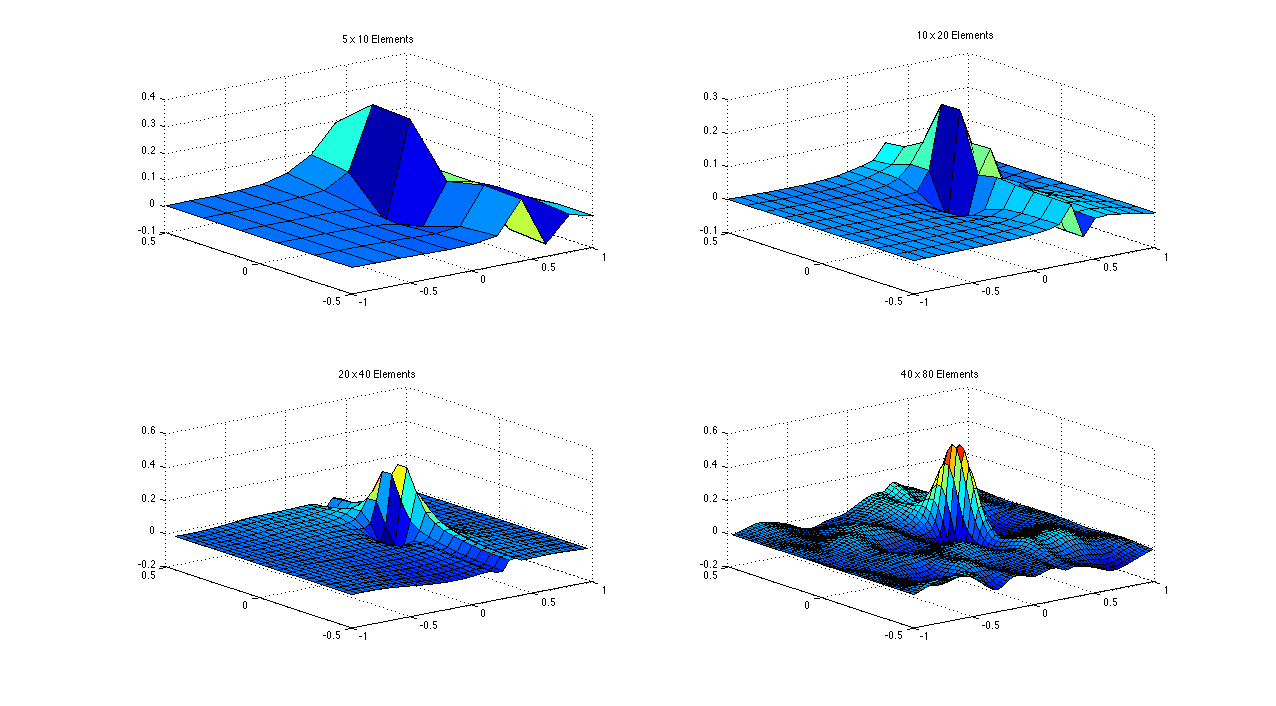
\includegraphics[width=\textwidth]{Figures/waves_in_cavity/waves_in_cavity.png}
\caption{H 3 components obtained after 100 seconds for gaussian function initial condition for various mesh refinements}
\label{WaveConv8}
\end{figure}

\begin{figure}
\includegraphics[width=\textwidth]{Figures/waves_in_cavity/waves_in_cavity_section_delta.png}
\label{WaveConv9}
\end{figure}

\begin{figure}
\includegraphics[width=\textwidth]{Figures/waves_in_cavity/waves_in_cavity_section_gauss.png}
\label{WaveConv10}
\end{figure}


% TODO - non-zero beta values

% TODO - CHECH THAT THIS IS ACTUALLY TRUE

% TODO - 

% TODO - why is this? Are gaussian initial conditions actually better in the long run??

%ConvergeOfWaveShapeWithH:
%-> this was measured after 10 cycles (is that enough for convergence? Who knows?)
%-> NOTE: I NEED TO RUN THIS WITH A HIGHER P AND A BETTER INITIAL CONDITION METHINKS....!! WAAAA!!!

% TODO - EVENTUALLY...! Convergence with P
% \begin{figure}
% \includegraphics[width=\textwidth]{Figures/2DPlate/WaveShapes/ConvergeOfWaveShapeWithP.png}
% \caption{Converge of wave shape with shape function order}
% \label{WaveConv3}
% \end{figure}

% \begin{figure}
% \includegraphics[width=\textwidth]{Figures/matlab/emptyplot.png}
% \caption{Convergence of wave shape measured at a point in space}
% \label{WaveConv4}
% \end{figure}

% \begin{figure}
% \includegraphics[width=\textwidth]{Figures/matlab/emptyplot.png}
% \caption{Error at same point in space as a function of time for various values of p (end every cycle)}
% \label{WaveConv5}
% \end{figure}

% \begin{figure}
% \includegraphics[width=\textwidth]{Figures/matlab/emptyplot.png}
% \caption{Error at same point in space as a function of time for various values of h (end every cycle)}
% \label{WaveConv6}
% \end{figure}

% \subsection{Propagation Constant}
% $\beta$ non-zero runs
% TODO: Change beta and show that the waves change as expected. Try to explain this in terms of the significance of Beta??
% \subsection{conclusion}

\section{FFT Spectrums}

Determination of frequency components of a time domain solution to maxwells equations is commonly done by a fourier transform to frequency space. The following spectrum was obtained by a Discrete Fourier Transform of a signal obtained from a finite element simulation. Peaks corrispond to resonant frequencies - known analytical values for resonant frequency are plotted for comparison.

\begin{figure}
\includegraphics[width=\textwidth]{Figures/matlab/Spectrums/GoodSpectrum.png}
\caption{Spectrum obtained by FFT from a timestep of 0.13E-03, 3,286,002 timesteps and 3200 elements. First order shape functions were used. A blackman window was used to reduce noise.}
\label{Spectrum1}
\end{figure}

% TODO - MAYBE DO WITHOUT A BLACKMAN WINDOW AND WITH A DELTA-FUNCTION INIT COND
% 
% \subsection{Window Functions}
% 
% \begin{figure}
% \includegraphics[width=\textwidth]{Figures/matlab/emptyplot.png}
% \caption{Spectrums with and without a window function}
% \label{WindowFFT1}
% \end{figure}
% 
% Quantify the noise (lowest possible cutoff frequency maybe, or cutoff freq difference)

\subsection{Peak Detection}

\subsubsection{Timestep And Cut-Off Frequencies}

% TODO - higher than Nyquist frequency??

% I need to determine a cut-off frequency?? What strategies do I have?
% 
% plot histogram for various differnt types of spectrum to show differences...! A BAD spectrum should have a BAD histogram
% Plot histogram to a number of ANALYTICAL frequencies with different samplings and spectrum richness (maybe) ??

The highest frequency component which can be indentified from a time-domain signal sampled at frequency $f_{s} = \frac{1}{T}$ where $T$ is the sampling time interval is given by:

$$f_{max} = \frac{f_s}{2} = \frac{1}{2T} $$

This introduces a theoretical upper bound on the spectrum obtained based on sampling frequency. In practice since the sampling interval used is the simulation time step then an upper limit will also be imposed by the stability criterion:

% TODO: STABILITY CRITERION

In practice upper limit for a wave domainated simulation will be the same as the time integration timestep of the simulation which is governed by stability conditions.

However as can be seen in \figref{Timestep1} a finite time-domain signal a sufficiently high sampling frequency will also introduces signal noise below this limit. Here the theoretical highest frequency is shown for each plot however we see degredation in the quality of the spectrum below this cut-off frequency. A sufficiently small timestep should be selected to allow the peaks to be clearly distingushed from spectrum noise. A practical measure of this degredation could be ratio of maximum height of spectral noise to minimum height of signal as shown in \figref{Timestep01}. 

%TODO - show this stuff for HARMINV too (to demonstrate that its relevant).

%TODO:CHECK THIS statement
In practice for these simple examples the time step required for solution stability was sufficient to identify the fundamental frequency of interest. However this could be a consideration if frequencies of interest were higher. %TODO - quantify this...! How much higher before it becomes comparible to stability

%TODO: QUANTIFY how much the timestep effects the ACTUAL frequencies (i.e. by finding the CLOSEST PEAK) - because the input signal is the same every time this probably won't be affected too much by frequency %(dt) for a long run. The real difficulty is in identifying the real and fictitious peaks which arise in the frequency determination. 

\begin{figure}
\includegraphics[width=\textwidth]{Figures/matlab/TimestepConvergence/Spectrums4up.png}
\caption{Spectrum obtained from the same signal using different sampling rates. Signal was generated with a 3200 element mesh and p-2 shape functions and a final time of 500s. The lowest sampling frequency corrisponds to the simulation timestep}
%TODO - how many elements.
%TODO - graph titles
\label{Timestep1}
\end{figure}

%TODO: Talk about cutoff frequencies and identifying resonant frequencies. Noise appears. How does this change with time. If I take a longer time for a noisy signal will this get better?

\begin{figure}
\includegraphics[width=\textwidth]{Figures/matlab/TimeStepConvergence/TimeStepConv.png}
\caption{Error in resonant frequency maximum against sampling period. Same signal used as in \figref{Timestep1}.}
%TODO - how many elements.
%TODO - graph titles
\label{Timestep01}
\end{figure}

%TODO - do this...!
%\begin{figure}
%\includegraphics[width=\textwidth]{Figures/matlab/emptyplot.png}
%\caption{Ratio of minimum resonant frequency component to maximum noise for the first 3 frequencies vs sampling frequency. Same signal used as in \figref{Timestep1}.}
% [or some other measure of how easy it is to extract frequencies - maybe based on histograms?? ]
%\label{Timestep0}
%\end{figure}

% \begin{figure}
% \includegraphics[width=\textwidth]{Figures/matlab/emptyplot.png}
% \caption{Frequencies obtained by sampling a analytical generated spectrum}
% \label{Timestep3}
% \end{figure}

\subsubsection{Peak Resolution}
Signals of finite length undergo a spectral leakage under fourier transform. As a result a shorter sample length results in noise appearing in the a spectrum with wider, badly-resolved peaks as shown in \figref{Period1}. A signal of length $5 \times 10^4$ is sufficient to capture the resonant frequencies with an error of $3 \times 10^6$.

%What is the minimum time I need to accurately capture ths signal at the accuracy required?
% note: more accuracy MEANS that we need much longer runs. No good having a more accurate wave...we also need a more accurate FFT...! So to capture a p3 accuracy with the same level of accuracy we need to run for how many time longer?? :)

% TODO Whats the minimum time (in general) that I need to remove the FFT transform error completely? :)

% TODO: Expression of dependence between timestep and resolution

\begin{figure}
\includegraphics[width=\textwidth]{Figures/matlab/PeriodConvergence/Spectrums4up.png}
\caption{Spectrum obtained from signal using different signal periods. Signal were generated with a timestep of 0.95E-02 using a mesh of 200 elements and p-1 shape functions}
\label{Period1}
\end{figure}

\begin{figure}
\includegraphics[width=\textwidth]{Figures/matlab/PeriodConvergence/PeriodConvergenceManual.png}
\caption{Error in calulations of resonant frequencies obtained against signal length}
\label{Period2}
\end{figure}

%TODO - same for analytical signals made of 1,3,10 \& 100 frequency components
%Use an analytical soltuion to identify (depending on richness of spectrum) the kind of accuracy I can expect to obtain after a FFT.

\subsubsection{Lorentzian Fitting}

In \figref{LorentzFit1} we see a number of resonant peaks fitted with a Lorentzian curve given by:

$$
L(x)=\frac{1}{\pi} \frac{\frac{1}{2}\Gamma}{ (x-x_0)^2 + (\frac{1}{2}\Gamma)^2}
$$

where $x_0$ is the center and $\Gamma$ is a width parameter. The Lorentzian function is commonly used to overcome the peak broadening associated with spectral leakage. In practice however fitting a lorentz curve reliably for narrow peak widths using a least squares method was complicated. However for peaks with less a bad resolution an improvement in the resolution was observed as shown in \figref{LorentzFit2}. This difficulty with fitting is one of the motivations for using the Filter Diagonalisation Method presented later.

\begin{figure}
\includegraphics[width=\textwidth]{Figures/matlab/Lorentz/LorentzFitManual.png}
\caption{Resonant peaks fitted with Lorentz curve at various periods showing the lorentz curve fits as spectrum resolution increases}
\label{LorentzFit1}
\end{figure}

\begin{figure}
\includegraphics[width=\textwidth]{Figures/matlab/Lorentz/LorentzFitPeriodConv.png}
\caption{Results showing the difference obtained by using a Lorentz fit at low periods. Resonably results can be obtained from very short runs in this way. However for longer runs the lorentz fit implementation was less reliable.}
\label{LorentzFit2}
\end{figure}

%\subsection{Spectral Richness}
%Dependece of spectral richness on initial conditions. Dependence of peak height and sharpness on intial conditions too [ maybe this should go somewhere else]

\begin{figure}
\includegraphics[width=\textwidth]{Figures/matlab/harminvr/InitCondHarminv.png}
\caption{Error vs Time for different types of initial conditions produced with FDM method}
\label{InitCond1}
\end{figure}
%delta/gaussian/multiple gaussians(10)/narrow gaussians

%Initial Condition Optimisation:
%\begin{figure}
%\includegraphics[width=\textwidth]{Figures/matlab/emptyplot.png}
%\caption{L2 norm error in the wave shapes against time for different types of initial conditions}
%\label{InitCond2}
%\end{figure}

% \subsubsection{Symmetry}
% \begin{figure}
% \includegraphics[width=\textwidth]{Figures/matlab/emptyplot.png}
% \caption{Spectrum from point with low symmetry and spectrum obtained from same simulation at a point with a high symmetry}
% \label{SymmDep1}
% \end{figure}

% Mesh dependence of initial condition:
% \begin{figure}
% \includegraphics[width=\textwidth]{Figures/matlab/emptyplot.png}
% \caption{Wave vs time for the same gaussian with different mesh sizes}
% \label{SymmDep2}
% \end{figure}

% TODO: Discussion on how finer meshes can capture a better spectrum due to initial condition containing a richer spectrum.

%\subsubsection{Components}
%
%\begin{figure}
%\includegraphics[width=\textwidth]{Figures/matlab/emptyplot.png}
%\caption{Spectrums obtained after 15 cycles}
%\label{CompDep2}
%\end{figure}

% TODO: Different components dominate in different cycles. Can I change the initial conditions to affect this?
%TODO - try to show that spectrums are richer for narrower gaussians??
%TODO(maybe): excite a single component... (?)

%\subsection{Obtaining Data}
%Quality factor...? Should I even mention this?

%\subsection{Conclusion}
%Limitations of FFT. Advantages of FFT (can see the spectrum)

\section{Filter Diagonalization Method}

% V. A. Mandelshtam and H. S. Taylor, "Harmonic inversion of time signals," J. Chem. Phys. 107 (17), 6756-6769 (1997). Erratum, ibid. 109 (10), 4128 (1998).
Limitations with FFT include the number of cycles required for optimal accuracy and the difficulty of lorentz fitting as the peak width gets narrower. The Filter Diagonalization is a popular method that addresses these issues and produces good results in much shorter times. The following are a list of results obtained using the Filter Diagonalization Method. However it is sometimes desirable to also use FFT in order to have a visible spectrum and a more complete picture of spectral content.

Signals were found to sometimes contain additional frequencies or to miss frequencies - but this could be corrected by using a higher number of basis functions.

%when signal consists of arbitrary number...
%TODO - getting rid of additional modes. When do these addtional modes appear? What happens if a run is too long? What happens if its too short.
%--> We get the Q for free (HOOOOW???)

% \begin{figure}
% \includegraphics[width=\textwidth]{Figures/matlab/emptyplot.png}
% \caption{Good spectrum and results obtained from FDM}
% \label{HarmivSpectrum1}
% \end{figure}
% 
% \begin{figure}
% \includegraphics[width=\textwidth]{Figures/matlab/emptyplot.png}
% \caption{Bad spectrum and results obtained from FDM method}
% \label{HarmivSpectrum2}
% \end{figure}
% TODO  FDM and how to optimise. Discuss crap spectrums producing usable results. Discuss fictitious/additional modes and how to get rid of them.......!!

\begin{figure}
\includegraphics[width=\textwidth]{Figures/matlab/harminvr/ConvergenceForDifferentDtHarminv.png}
\caption{Convergence of FDM results for various signal lengths for two different sampling intervals. Note that these sampling intervals also corrispond to time integration timestep. Results are compared with convergence results obtained from the same data for FFT.}
\label{HarmivSpectrum3}
\end{figure}

\begin{figure}
\includegraphics[width=\textwidth]{Figures/matlab/harminvr/HarminvConvergencePlots.png}
\caption{Error in FDM calculations obtained by mesh refinement using 50, 200 and 800 elements for p1 calculations}
\label{HarmivSpectrum4}
\end{figure}

%TODO - Harminv is x times better. Compare them...! Identifying fictitious modes

%\subsection{Initial Condition Dependence}
%show different initial conditions (gaussian, delta, sigma, number of gaussians) - same plot as before with Harminv. Demonstrate difference in initial conditions.

%TODO: is FDM more or less sensitive to initial condition time steps?

%\subsection{Window Functions}

% \begin{figure}
% \includegraphics[width=\textwidth]{Figures/matlab/emptyplot.png}
% \caption{Convergence with window length}
% \label{HarmivWindow1}
% \end{figure}

% \begin{figure}
% \includegraphics[width=\textwidth]{Figures/matlab/emptyplot.png}
% \caption{Convergence with window start time for different p/h}
% \label{HarmivWindow2}
% \end{figure}

% \input{./Chapters/Appendix.2D_Plate_notes}
% % Chapter 1

\chapter{Numerical FDTD 1D Simulations} % Write in your own chapter title
\label{Chapter5}
\lhead{Chapter 5. \emph{Numerical FDTD 1D Simulations}} % Write in your own chapter title to set the page header

Numerical simulations were performed using a simple finite difference 1D time domain solver by propagating a wave of the form:

$$
sin(2 \pi f (t - x))
$$

The code used was a simple FDTD 1D implementation written in matlab.

The domain used for all simulations was [0,20] and the waves obtained were compared to the analytical solutions to produce an L2 norm of the resulting wave. The initial conditions used were zero in the whole domain and dirichlet boundary conditions were introduced on the left boundary - however as can be noted from the analytical form of the wave this does not introduce a discontinuity in the solution (at least not to first order). No boundary condition is set on the right hand side of the domain - but the simulation was stopped before the wave reached the far side.
All analysis was done on the 3rd component of the TE mode (E3) which is continuous.
%TODO - verify this...!
Unless otherwise specified the frequency used was f=2, the domain used is of length L=100 with final time at 0.9L with the signal captured at x=20.
% TODO - verify this...!

\begin{figure}
\includegraphics[width=\textwidth]{Figures/1D_FD_propagation/L2_norm_only_dt_refinement/aggregate.png}
\caption{Various mesh size were selected and kept constant while dt was refined. The lower bound on dt is set purely by computational time with no stability constraints. The L2 norm error both in the wave shape over the domain at the final time and in a signal sampled at a selected point at intervals of dt is shown.}
\label{dt_refinement}
\end{figure}

\begin{figure}
\includegraphics[width=\textwidth]{Figures/1D_FD_propagation/L2_norm_only_dx_refinement/aggregate_2.png}
\caption{A similar analysis to figure \ref{dt_refinement} shows dx refinement for fixed dt values. In this case the stability condition and the choice of dt sets a lower bound of dt (dt=dx).}
\end{figure}

% \begin{figure}
% \includegraphics[width=\textwidth]{Figures/1D_FD_propagation/L2_norm_only_dx_refinement/aggregate_10.png}
% \caption{dx refinement for various fixed dt values for frequency f=10. Note there is a lower bound of dt=dx in this case for stability.}
% \end{figure}
% 
% \begin{figure}
% \includegraphics[width=\textwidth]{Figures/1D_FD_propagation/L2_norm_only_dx_refinement/aggregate_20.png}
% \caption{dx refinement for various fixed dt values for frequency f=20. Note there is a lower bound of dt=dx in this case for stability.}
% \end{figure}

\begin{figure}
\includegraphics[width=\textwidth]{Figures/1D_FD_propagation/L2_norm_vs_dx_C_0_8/aggregate_2.png}
\caption{The L2 norm error in the wave and signal shapes with uniform dx and dt (by a factor of 2) refinement using a consisten value of C=0.8. The plots are shown against dx however there is also an implied refinement of dt.}
\end{figure}

\begin{figure}
    \begin{center}
        \subfigure[FFT calculations]{
            \label{FTTC}
            \includegraphics[width=0.6\textwidth]{Figures/1D_FD_propagation/Convergence_plots_with_C/error_from_spectrum_vs_c.png}
        }
        
        \subfigure[FDM calculations]{
            \includegraphics[width=0.6\textwidth]{Figures/1D_FD_propagation/Convergence_plots_with_C/error_from_fdm_vs_c.png}
            \label{FDMC}
        }
        \caption{Error in frequency calculation for different values of C. In this case the refinement was performed by setting dx=0.1 and choosing a dt for the selected C. Then allowing uniform refinement of dx and dt simultaneously by a factor of 2 to preserve C.}
    \end{center}
    
\end{figure}


\begin{figure}
\includegraphics[width=\textwidth]{Figures/1D_FD_propagation/Convergence_plots_with_dx/aggregate_2.png}
\caption{This plots show the relative error in frequency converging with dx for selected constant values of dt for a frequency f=2}
\end{figure}

\begin{figure}
\includegraphics[width=\textwidth]{Figures/1D_FD_propagation/Convergence_plots_with_dx/aggregate_20.png}
\caption{This plots show the relative error in frequency converging with dx for selected constant values of dt for a frequency f=20}
\end{figure}

\begin{figure}
\includegraphics[width=\textwidth]{Figures/1D_FD_propagation/Convergence_plots_with_dx/aggregate_10.png}
\caption{This plots show the relative error in frequency converging with dx for selected constant values of dt for a frequency f=10}
\end{figure}

\begin{figure}
\includegraphics[width=\textwidth]{Figures/1D_FD_propagation/PeriodStudy_long_run/FDM_and_FFT_errors.png}
\caption{A brief period study to select the time required for sufficient accuracy of FDM and FFT methods}
\end{figure}

% % Chapter 1

\chapter{Dispersive Materials} % Write in your own chapter title
\label{Chapter4}
\lhead{Chapter 3. \emph{Dispersive Materials}} % Write in your own chapter title to set the page header

In general light travels as a polychromatic waves - containing several different frequencies. In general each frequency travels at a different speed in a medium. The material parameters depend on the frequency of the radiation.

\section{The Drude Model}

The drude model was initially proposed in *** based on the kinetic theory of gases [citation]. In the drude model a metal is modelled as a fixed lattice of positively charged ions in a sea of negatively charged valance or conduction (in a metal) electrons which are free to move.

%TODO  - direct quote - IntriaPaper DGTD dispersive
Assumptions:
• The electrons description is non-relativistic;
• The only considered interactions are the electron/wave and the electron/ion ones;
• The electron/ion collisions are instantaneous and random events, and their probability of happening during a dt amount of time is equal to dt 1;
τf
• After an electron/ion collision, the new velocity and direction of the electron are inde-
pendant of those before the collision.


Under these hypotheses, the frequency dependence of the medium permittivity can be de- duced from the equations of motion.
%TODO - end direct quote

When subjected to a constant external electric field $\mathbf{E}$ the displacement of the heavy valence ions from their equilibtrium position is assume to be negligable whilst the electrons move significantly from their equilibrium position in response to an externally applied field. This results in an additional electric field $\mathbf{P}$ due to material response to the applied field $\mathbf{E}$ orientated in the opposite direction resulting in a total field given by the electric displacement field $\mathbf{D}$ where:

$$
\mathbf{D} = \epsilon_0 \mathbf{E} + \mathbf{P}
$$

Note that usually the signs of $\mathbf{P}$ and $\mathbf{E}$ will be opposite - resulting in an induced field that opposes the applied field and consequentially a reduced field in the medium.

% TODO: Is it accurate to describe the displacement electric field as the total electric field....?

For a constant or slow-varying field with respect to the material response time $\tau$ the polarisation of the material $\mathbf{P}$ will be proportional to the applied electric field and can be described as a constant of proportionality $\chi$, known as the electric susceptibility which describes how susceptible the material is to polarisation. $\mathbf{P}$ can be written as:

$$
\mathbf{P} = \chi \mathbf{E}
$$

$\chi$ is not always constant - and in general is a tensor.

Furthermore the movement of electrons from their zero-field equlibrium positions to the equilibrium positions under the applied field $\mathbf{E}$ could take some finite time $\tau$ (characteristic time). For an applied electric field $\mathbf{E}$ which is changing sufficiently quickly this time needs to be accounted for and $\chi$ may not be described as simply by a constant since it clearly depends on the history of the mediums polarisation.

TODO - derivation from equations of motion to conservation form....find a nice way of doing this....

\section{Beyond the Drude Model}
- what about the Lorentz model
- Drude/Lorentz model
- Debye model
- Generalised dispersion

\section{Non-Dimensionalization of Drude Model}
We define the following dimensionless units for a system with a characteristic length L:
$$
t' = \frac{ct}{L}
$$

$$
\mathbf{x'} = \frac{\mathbf{x}}{L}
$$

$$
\mathbf{E'} = \mathbf{E}\sqrt{\frac{\epsilon_0}{\mu_0}}
$$

$$
\mathbf{J'} = L\mathbf{J}
$$

\section{Results}

\begin{figure}
\includegraphics[width=\textwidth]{Figures/2D_DispersivePlate/convergenceStudies/convergenceAllComponents/L2vsH_TE.png}
\caption{Convergence plots fo TE validation case}
\end{figure}

\begin{figure}
\includegraphics[width=\textwidth]{Figures/2D_DispersivePlate/convergenceStudies/convergenceAllComponents/L2vsH_TM.png}
\caption{Convergence plots fo TM validation case}
\end{figure}

\begin{figure}
\includegraphics[width=\textwidth]{Figures/2D_DispersivePlate/convergenceStudies/convergenceAllComponents/L2vsH.png}
\caption{Convergence plots for all component case}
\end{figure}

\clearpage
\section{Error Plots}

\begin{figure}
\includegraphics[width=\textwidth]{Figures/2D_DispersivePlate/convergenceStudies/ErrorPlots/convergencePlots_dat_dispersiveSquareQUA_H3_p3_TE_iComp1.png}
\end{figure}

\begin{figure}
\includegraphics[width=\textwidth]{Figures/2D_DispersivePlate/convergenceStudies/ErrorPlots/convergencePlots_dat_dispersiveSquareQUA_H3_p3_TE_iComp2.png}
\end{figure}

\begin{figure}
\includegraphics[width=\textwidth]{Figures/2D_DispersivePlate/convergenceStudies/ErrorPlots/convergencePlots_dat_dispersiveSquareQUA_H3_p3_TE_iComp3.png}
\end{figure}

\begin{figure}
\includegraphics[width=\textwidth]{Figures/2D_DispersivePlate/convergenceStudies/ErrorPlots/convergencePlots_dat_dispersiveSquareQUA_H3_p4_TE_iComp1.png}
\end{figure}

\begin{figure}
\includegraphics[width=\textwidth]{Figures/2D_DispersivePlate/convergenceStudies/ErrorPlots/convergencePlots_dat_dispersiveSquareQUA_H3_p4_TE_iComp2.png}
\end{figure}

\begin{figure}
\includegraphics[width=\textwidth]{Figures/2D_DispersivePlate/convergenceStudies/ErrorPlots/convergencePlots_dat_dispersiveSquareQUA_H3_p4_TE_iComp3.png}
\end{figure}

\begin{figure}
\includegraphics[width=\textwidth]{Figures/2D_DispersivePlate/convergenceStudies/ErrorPlots/convergencePlots_dat_dispersiveSquareQUA_H3_p4_TM_iComp1.png}
\end{figure}

\begin{figure}
\includegraphics[width=\textwidth]{Figures/2D_DispersivePlate/convergenceStudies/ErrorPlots/convergencePlots_dat_dispersiveSquareQUA_H3_p4_TM_iComp2.png}
\end{figure}

\begin{figure}
\includegraphics[width=\textwidth]{Figures/2D_DispersivePlate/convergenceStudies/ErrorPlots/convergencePlots_dat_dispersiveSquareQUA_H3_p4_TM_iComp3.png}
\end{figure}

\begin{figure}
\includegraphics[width=\textwidth]{Figures/2D_DispersivePlate/convergenceStudies/ErrorPlots/convergencePlotsTRI_TM_dat_dispersiveSquareTRI_H5_p3_TM_iComp1.png}
\end{figure}

\begin{figure}
\includegraphics[width=\textwidth]{Figures/2D_DispersivePlate/convergenceStudies/ErrorPlots/convergencePlotsTRI_TM_dat_dispersiveSquareTRI_H5_p3_TM_iComp2.png}
\end{figure}

\begin{figure}
\includegraphics[width=\textwidth]{Figures/2D_DispersivePlate/convergenceStudies/ErrorPlots/convergencePlotsTRI_TM_dat_dispersiveSquareTRI_H5_p3_TM_iComp3.png}
\end{figure}

\begin{figure}
\includegraphics[width=\textwidth]{Figures/2D_DispersivePlate/convergenceStudies/ErrorPlots/dispersiveSquareQUA_H1_p3_TE_iComp1.png}
\end{figure}

\begin{figure}
\includegraphics[width=\textwidth]{Figures/2D_DispersivePlate/convergenceStudies/ErrorPlots/dispersiveSquareQUA_H1_p3_TE_iComp2.png}
\end{figure}

\begin{figure}
\includegraphics[width=\textwidth]{Figures/2D_DispersivePlate/convergenceStudies/ErrorPlots/dispersiveSquareQUA_H1_p3_TE_iComp3.png}
\end{figure}

\clearpage

\begin{figure}
\includegraphics[width=\textwidth]{Figures/2D_DispersivePlate/convergenceStudies/ErrorPlots/dispersiveSquareQUA_H3_p1_TE_iComp1.png}
\end{figure}

\begin{figure}
\includegraphics[width=\textwidth]{Figures/2D_DispersivePlate/convergenceStudies/ErrorPlots/dispersiveSquareQUA_H3_p1_TE_iComp2.png}
\end{figure}

\begin{figure}
\includegraphics[width=\textwidth]{Figures/2D_DispersivePlate/convergenceStudies/ErrorPlots/dispersiveSquareQUA_H3_p1_TE_iComp3.png}
\end{figure}

\begin{figure}
\includegraphics[width=\textwidth]{Figures/2D_DispersivePlate/convergenceStudies/ErrorPlots/dispersiveSquareQUA_H3_p3_TE_iComp1.png}
\end{figure}

\begin{figure}
\includegraphics[width=\textwidth]{Figures/2D_DispersivePlate/convergenceStudies/ErrorPlots/dispersiveSquareQUA_H3_p3_TE_iComp2.png}
\end{figure}

\begin{figure}
\includegraphics[width=\textwidth]{Figures/2D_DispersivePlate/convergenceStudies/ErrorPlots/dispersiveSquareQUA_H3_p3_TE_iComp3.png}
\end{figure}

\begin{figure}
\includegraphics[width=\textwidth]{Figures/2D_DispersivePlate/convergenceStudies/ErrorPlots/dispersiveSquareQUA_H3_p3_TM_iComp1.png}
\end{figure}

\begin{figure}
\includegraphics[width=\textwidth]{Figures/2D_DispersivePlate/convergenceStudies/ErrorPlots/dispersiveSquareQUA_H3_p3_TM_iComp2.png}
\end{figure}

\begin{figure}
\includegraphics[width=\textwidth]{Figures/2D_DispersivePlate/convergenceStudies/ErrorPlots/dispersiveSquareQUA_H3_p3_TM_iComp3.png}
\end{figure}

\begin{figure}
\includegraphics[width=\textwidth]{Figures/2D_DispersivePlate/convergenceStudies/ErrorPlots/dispersiveSquareTRI_H5_p3_TE_iComp1.png}
\end{figure}

\begin{figure}
\includegraphics[width=\textwidth]{Figures/2D_DispersivePlate/convergenceStudies/ErrorPlots/dispersiveSquareTRI_H5_p3_TE_iComp2.png}
\end{figure}

\begin{figure}
\includegraphics[width=\textwidth]{Figures/2D_DispersivePlate/convergenceStudies/ErrorPlots/dispersiveSquareTRI_H5_p3_TE_iComp3.png}
\end{figure}

\begin{figure}
\includegraphics[width=\textwidth]{Figures/2D_DispersivePlate/convergenceStudies/ErrorPlots/moreSnapshotsForErrorMovie_dat_dispersiveSquareQUA_H3_p3_TM_iComp1.png}
\end{figure}

\begin{figure}
\includegraphics[width=\textwidth]{Figures/2D_DispersivePlate/convergenceStudies/ErrorPlots/moreSnapshotsForErrorMovie_dat_dispersiveSquareQUA_H3_p3_TM_iComp2.png}
\end{figure}

\begin{figure}
\includegraphics[width=\textwidth]{Figures/2D_DispersivePlate/convergenceStudies/ErrorPlots/moreSnapshotsForErrorMovie_dat_dispersiveSquareQUA_H3_p3_TM_iComp3.png}
\end{figure}
% \chapter{MPI Profiling} % Write in your own chapter title
\label{Chapter8}
\lhead{Chapter 8. \emph{MPI Profiling}} % Write in your own chapter title to set the page header

\section{Solution comparions at a point}

\subsection{Scattering}

\begin{figure}[!htb]
\includegraphics[width=0.4\textwidth]{Figures/MPI/collectedResults/Scattering_TRI_all_figs/UElem40Err/h1_pml1.png}
\includegraphics[width=0.4\textwidth]{Figures/MPI/collectedResults/Scattering_TRI_all_figs/UElem40Err/h1_pml3.png}
\includegraphics[width=0.4\textwidth]{Figures/MPI/collectedResults/Scattering_TRI_all_figs/UElem40Err/h1_pml0.png}
\includegraphics[width=0.4\textwidth]{Figures/MPI/collectedResults/Scattering_TRI_all_figs/UElem40Err/h1_pml2.png}

\caption{Error in solution for all PMLs with mesh H1}
\end{figure}

\begin{figure}[!htb]
\includegraphics[width=0.4\textwidth]{Figures/MPI/collectedResults/Scattering_TRI_all_figs/UElem40Err/h2_pml0.png}
\includegraphics[width=0.4\textwidth]{Figures/MPI/collectedResults/Scattering_TRI_all_figs/UElem40Err/h2_pml1.png}
\includegraphics[width=0.4\textwidth]{Figures/MPI/collectedResults/Scattering_TRI_all_figs/UElem40Err/h2_pml2.png}
\includegraphics[width=0.4\textwidth]{Figures/MPI/collectedResults/Scattering_TRI_all_figs/UElem40Err/h2_pml3.png}
\caption{Error in solution for all PMLs with mesh H2}
\end{figure}


\begin{figure}[!htb]
\includegraphics[width=0.4\textwidth]{Figures/MPI/collectedResults/Scattering_TRI_all_figs/UElem40Err/h3_pml0.png}
\includegraphics[width=0.4\textwidth]{Figures/MPI/collectedResults/Scattering_TRI_all_figs/UElem40Err/h3_pml1.png}
\includegraphics[width=0.4\textwidth]{Figures/MPI/collectedResults/Scattering_TRI_all_figs/UElem40Err/h3_pml2.png}
\includegraphics[width=0.4\textwidth]{Figures/MPI/collectedResults/Scattering_TRI_all_figs/UElem40Err/h3_pml3.png}
\caption{Error in solution for all PMLs with mesh H3}
\end{figure}

\clearpage
\subsection{Unit Cube (PYR)}

\begin{figure}[!htb]
\includegraphics[width=0.4\textwidth]{Figures/MPI/checkUElem40_unitCube/pOption_1-inputFileDAT_dat_unitCubePYR_H1-UElem40.png}
\includegraphics[width=0.4\textwidth]{Figures/MPI/checkUElem40_unitCube/pOption_1-inputFileDAT_dat_unitCubePYR_H2-UElem40.png}
\includegraphics[width=0.4\textwidth]{Figures/MPI/checkUElem40_unitCube/pOption_1-inputFileDAT_dat_unitCubePYR_H3-UElem40.png}
\caption{Value of solution checked at a given node for a unit cube for PYR H1-3, p1}
\end{figure}


\begin{figure}[!htb]
\includegraphics[width=\textwidth]{Figures/MPI/collectedResults/unitCubeAll.figs/unitCubeConv.png}
\caption{figure}
\end{figure}

\begin{figure}[!htb]
\includegraphics[width=\textwidth]{Figures/MPI/collectedResults/unitCubeAll.figs/unitCubeConvNDOF.png}
\caption{figure}
\end{figure}


\begin{figure}[!htb]
\begin{tabular}{| l || c | c | c |}
\hline
\multicolumn{4}{|c|}{PYR p = 1} \\
\hline
U1 & 1.53 & 2.26 & 2.22 \\
U2 & 1.60 & 2.34 & 2.28 \\
U3 & 1.53 & 2.26 & 2.22 \\
U4 & 1.59 & 2.33 & 2.27 \\
U5 & 1.10 & 1.99 & 2.05 \\
U6 & 1.59 & 2.33 & 2.27 \\
\hline
\hline
\multicolumn{4}{|c|}{PYR p = 2} \\
\hline
U1 & 3.05 & 2.93 & \\
U2 & 3.31 & 3.00 & \\
U3 & 3.05 & 2.93 & \\
U4 & 3.27 & 2.99 & \\
U5 & 2.52 & 2.84 & \\
U6 & 3.27 & 2.99 & \\
\hline   
\end{tabular}
\end{figure}

\clearpage
\section{CPU times}
\subsection{Scattering Example}

\begin{figure}[!htb]
\includegraphics[width=\textwidth]{Figures/MPI/collectedResults/Scattering_TRI_all_figs/cpuTimeComparison_pml0.png}
\caption{CPU time comparison against previous serial code for 2D circle scattering for 4-nodes. Example shows pml=0 but same result obtained for other PMLs}
\end{figure}

\begin{figure}[!htb]
\includegraphics[width=\textwidth]{Figures/MPI/timing-progressive/timingSameProblem/absolute-time.png}
\caption{figure}
\end{figure}

\begin{figure}[!htb]
\includegraphics[width=\textwidth]{Figures/MPI/timing-progressive/timingSameProblem/fraction-of-single-node-time.png}
\caption{figure}
\end{figure}


\begin{figure}[!htb]
\includegraphics[width=\textwidth]{Figures/MPI/timing-progressive/timingSameProblem/multiple-of-single-node-time.png}
\caption{figure}
\end{figure}


\begin{figure}[!htb]
\includegraphics[width=\textwidth]{Figures/MPI/timing-progressive/timingSameProblem/single-node-time-over-time-per-cycle.png}
\caption{figure}
\end{figure}

\clearpage
\subsection{Unit Cube}

\begin{figure}[!htb]
\includegraphics[width=\textwidth]{Figures/MPI/collectedResults/unitCubeAll.figs/cpuTimeComparison.png}
\caption{Unit cube cpu for each cycle (compared to original serial code) for 5-nodes}
\end{figure}

\begin{figure}[!htb]
\includegraphics[width=\textwidth]{Figures/MPI/collectedResults/unitCubeAll.figs/unitCubeConvCPU.png}
\caption{figure}
\end{figure}


% % Chapter 1

\chapter{Numerical DGTD 2D Simulations} % Write in your own chapter title
\label{Chapter6}
\lhead{Chapter 6. \emph{Numerical DGTD 2D Simulations}} % Write in your own chapter title to set the page header

A simple 2D plane wave was propagated in a rectangular free-space 2D waveguide of width 0.5 and length L. All simulations are performed with p=1.
The same timestep was used for all simulations of 0.5E-3 (this is consistent with timectt=0.2 for the smallest element size used) and length of a cycle = 1.

\begin{figure}
\includegraphics[width=\textwidth]{Figures/2D_DGTD_RectWaveGuide/timestepTooLarge/1E-3/storeFrames/pml0.5/L2ConvPlot_pmls_xmax_half_iframe_30.png}
\caption{Domain of size 0.5x0.5 with a PML of length shown in legend after 3 cycles [run too short]}
\end{figure}

\begin{figure}
\includegraphics[width=\textwidth]{Figures/2D_DGTD_RectWaveGuide/timestepTooLarge/1E-3/storeFrames/pml1.5/L2ConvPlot_pml1_point_5_xmax1_iframe100.png}
\caption{Domain of size 0.5x1.5 with a PML of length shown in legend after 10 cycles}
\end{figure}

\begin{figure}
\includegraphics[width=\textwidth]{Figures/2D_DGTD_RectWaveGuide/timestepTooLarge/1E-3/storeFrames/pml1.5/L2ConvPlot_pml1_point_5_xmax0_point_5_iframe100.png}
\caption{L2 norm for domain of size 0.5x1.5 with a PML of length shown in legend with error measured only on interval [0,0.5] again over 10 cycles}
\end{figure}

\begin{figure}
\includegraphics[width=\textwidth]{Figures/2D_DGTD_RectWaveGuide/timestepTooLarge/1E-3/storeFrames/pml1.5/L2ConvPlot_pml1_point_5_xmax1_iframe100.png}
\caption{L2 norm for domain of size 0.5x1.5 with a PML of length shown in legend with error measured only on interval [0,1] again over 10 cycles}
\end{figure}

\begin{figure}
\includegraphics[width=\textwidth]{Figures/2D_DGTD_RectWaveGuide/timestepTooLarge/0.5E-3/p1/0.5x1/L2Conv.png}
\caption{L2 Convergence with time for L=1 with various element refinements. The number of elements is shown in the figure}
\end{figure}

\begin{figure}
\includegraphics[width=\textwidth]{Figures/2D_DGTD_RectWaveGuide/timestepTooLarge/0.5E-3/p1/0.5x1/L2ConvPlot.png}
\caption{Convergence plot with time obtained from the final timestep (T=10) for L=1}
\end{figure}

\begin{figure}
\includegraphics[width=\textwidth]{Figures/2D_DGTD_RectWaveGuide/timestepTooLarge/0.5E-3/p1/0.5x1.5/L2Conv.png}
\caption{L2 Convergence with time for L=1.5 with various element refinements. The number of elements is shown in the figure}
\end{figure}

\begin{figure}
\includegraphics[width=\textwidth]{Figures/2D_DGTD_RectWaveGuide/timestepTooLarge/0.5E-3/p1/0.5x1.5/L2ConvPlot.png}
\caption{Convergence plot with time obtained from the final timestep (T=10) for L=1.5}
\end{figure}

\begin{figure}
\includegraphics[width=\textwidth]{Figures/2D_DGTD_RectWaveGuide/timestepTooLarge/0.5E-3/p1/0.5x1.5_pml/FinalRun_16x48.png}
\caption{Wave shapes and errors for L=1.5 with attempt to introduce PML with 15x48 elements, p=1}
\end{figure}

\begin{figure}
\includegraphics[width=\textwidth]{Figures/2D_DGTD_RectWaveGuide/timestepTooLarge/0.5E-3/p1/0.5x5/L2ConvWithTime.png}
\caption{L2 norm convergence for different number of element with time for L=5. This shows less error due to reflection.}
\end{figure}

\begin{figure}
\includegraphics[width=\textwidth]{Figures/2D_DGTD_RectWaveGuide/timestepTooLarge/0.5E-3/p1/0.5x5/L2ConvWithH.png}
\caption{Convergence of L2 norm for the wave at the final time T=10 with element size h with L=5}
\end{figure}

\begin{figure}
\includegraphics[width=\textwidth]{Figures/2D_DGTD_RectWaveGuide/timestepTooLarge/0.5E-3/p1/0.5x5/FinalRun_16x160.png}
\caption{Numerical solution, Analytical solution and absolute error at every point int he domain for 16x160 elements with L=5}
\end{figure}

\begin{figure}
\includegraphics[width=\textwidth]{Figures/2D_DGTD_RectWaveGuide/timestepTooLarge/0.5E-3/p1/0.5x5/FinalRun_8x80.png}
\caption{Numerical solution, Analytical solution and absolute error at every point int he domain for 8x80 elements with L=5}
\end{figure}



%% ----------------------------------------------------------------
% Now begin the Appendices, including them as separate files

\addtocontents{toc}{\vspace{2em}} % Add a gap in the Contents, for aesthetics

\appendix % Cue to tell LaTeX that the following 'chapters' are Appendices

%% Appendix A

\chapter{Appendix Title Here}
\label{AppendixA}
\lhead{Appendix A. \emph{Appendix Title Here}}

Write your Appendix content here.	% Appendix Title

%\input{./Appendices/AppendixB} % Appendix Title

%\input{./Appendices/AppendixC} % Appendix Title

\addtocontents{toc}{\vspace{2em}}  % Add a gap in the Contents, for aesthetics
\backmatter

%% ----------------------------------------------------------------
\label{Bibliography}
\lhead{\emph{Bibliography}}  % Change the left side page header to "Bibliography"

\bibliography{Thesis} % The references (bibliography) information are stored in the file named "Thesis.bib"
\bibliographystyle{unsrt}

\end{document}  % The End
%% ----------------------------------------------------------------

%%% Local Variables:
%%% mode: latex
%%% TeX-master: t
%%% End:
